% !TeX program = xelatex
\documentclass[12pt,a4paper]{ctexart}

\usepackage{geometry}
\geometry{a4paper,left=2.8cm,right=2.8cm,top=2.2cm,bottom=2.2cm}
\usepackage{graphicx}
\usepackage{booktabs}
\usepackage{longtable}
\usepackage{array}
\usepackage{enumitem}
\usepackage{amsmath}
\usepackage{listings}
\usepackage{xcolor}
\usepackage{caption}
\captionsetup{labelsep=quad}
\usepackage{float}
\usepackage[hidelinks]{hyperref}

\captionsetup{font=small,labelfont=bf}
\lstset{
  basicstyle=\small\ttfamily,
  breaklines=true,
  columns=fullflexible,
  frame=single,
  framesep=4pt,
  rulecolor=\color{gray!45},
  backgroundcolor=\color{gray!6},
  showstringspaces=false,
  keepspaces=true
}
\setlist{nosep,leftmargin=2em}
\emergencystretch=3em

\title{\textbf{基于规则引擎与大语言模型的党员发展材料智能审核工作台设计与实现}}
\author{AI 应用开发项目组}
\date{2026 年 10 月}

% MH-FLOAT-TUNE 受控浮动调参（防整页空白/一页一图）
\usepackage[section]{placeins}
\renewcommand{\topfraction}{0.92}
\renewcommand{\bottomfraction}{0.9}
\renewcommand{\textfraction}{0.06}
\renewcommand{\floatpagefraction}{0.72}
\renewcommand{\dbltopfraction}{0.92}
\renewcommand{\dblfloatpagefraction}{0.72}
\setcounter{topnumber}{3}
\setcounter{bottomnumber}{2}
\setcounter{totalnumber}{4}
\begin{document}
\maketitle
\thispagestyle{empty}

\begin{abstract}
\addcontentsline{toc}{section}{摘要}

高校党员发展工作程序性强、材料种类多、时间节点密、规范要求严。一名发展对象从递交入党申请书到预备党员转正，需要经历五个发展阶段、跨越两年以上，形成入党申请书、思想汇报、写实簿、自传、入党志愿书等数十份材料，并依次接受党支部初审、支部交叉互查、学院党委复审与学校组织部备案。传统审核依赖党务工作人员逐份逐页人工翻阅，工作量大、标准不统一，时间逻辑难以逐一核验，问题反馈也不及时。

本文设计并实现了一套面向高校党组织的党员发展材料智能审核工作台。系统以 PostgreSQL 为数据底座，后端以 FastAPI 构建统一的接口层与业务服务层，前端以 React 单页应用分别实现学生端与审核端。人工智能能力被组织为\textbf{解析、理解、校验、汇总、结论五阶段}：解析阶段支持 PDF、Word 与图片扫描件的文本提取；理解阶段完成材料种类识别、要素抽取与跨材料时间节点合并；校验阶段由规则引擎执行完整性、时间逻辑、形式规范与内容规范四类检查，其中时间逻辑基于一套\textbf{可配置的时间规则领域特定语言}；汇总阶段对问题去重分级并生成标准化修改建议；结论阶段输出参考意见，并按置信度与节点冲突判定是否需要人工接管。

系统实现了五级审核流程与完整的整改回路，学生可对照问题清单逐条整改后重新提交，由系统自动复核。为保证结果可追溯，流转、审核、导出与规则变更均写入审计日志，报告同时记录所用规则版本与模型名称。AI 结论只作参考，最终结论由审核人员确认，需要人工接管时必须写明理由方可放行。内容语义核查已接入提示词模板，并以本地模拟端点验证了配置、调用、降级与追溯链路；后端回归 45 项、HTTP 全链路 23 项断言与接口探针 36 项共 104 项检查全部通过，规则引擎稳定识别出四类问题，扫描件识别与批量审核并发场景均经专项验证，能够明显减少逐页审阅的工作量。
\end{abstract}

\vspace{1em}
\noindent\textbf{关键词：} 党员发展材料；智能审核；规则引擎；领域特定语言；文档解析；OCR；大语言模型；人工接管

\section*{Abstract}
\addcontentsline{toc}{section}{Abstract}

This report presents an AI-assisted review and verification workstation for the materials produced during the development of Party members in Chinese universities. The system is built with a FastAPI backend, a React single-page frontend and a PostgreSQL database, and organizes its AI capability as a five-stage pipeline --- parsing, understanding, checking, aggregation and conclusion. A configurable domain-specific language drives the time-logic checks, while rule-based completeness, format and content checks, together with optional large language model support, produce graded issues and standardized revision suggestions. Content semantic checks are wired through a prompt-template driven LLM adapter, which degrades to skipped rules on failure and records the model name in each report. A five-level review chain with human-in-the-loop handover, full audit trails and rule-version snapshots guarantees that AI output remains advisory. Regression testing reports 104 passed checks with zero failures, comprising 45 backend tests, 23 end-to-end assertions and 36 live API probes.

\vspace{0.6em}
\noindent\textbf{Keywords:} Party member development materials; intelligent review; rule engine; DSL; document parsing; OCR; large language model; human-in-the-loop

\clearpage
\section{绪论}

\subsection{选题背景与意义}

发展党员是党的建设的源头工程和基础工程，必须严格程序、严守标准。按照《中国共产党发展党员工作细则》的要求，发展一名党员需要经过"申请入党、确定入党积极分子、确定发展对象、接收预备党员、预备党员转正"五个阶段，每个阶段都有明确的材料清单、时间间隔与程序要求：递交入党申请书后一个月内党组织要派人谈话，确定为入党积极分子后要经过一年以上的培养考察才能确定为发展对象，接收预备党员前要完成政治审查与公示，预备期满要按期讨论转正并报上级党委审批。与之对应，一名发展对象在整个培养周期中会形成入党申请书、思想汇报、培养教育考察写实簿、自传、政治审查材料、入党志愿书、公示材料、各类会议记录与审批意见等数十份材料，其中既有打印件也有手写件，既有电子文档也有纸质扫描件。

高校每年发展党员数量大、批次集中，材料审核工作主要依赖学院党委和党支部的党务工作人员逐份逐页人工完成，面临三方面突出困难。一是\textbf{工作量大}：一名学生的档案动辄上百页，一个学院一次集中审核往往涉及数百名学生，人工审阅耗时巨大；二是\textbf{标准难以完全统一}：材料种类是否齐全、时间节点是否满足培养周期、落款与印章是否规范、政治表述是否准确，高度依赖审核人员的经验；三是\textbf{时间逻辑难以逐一核验}：培养周期、阶段间隔、公示时限等时间类要求散落在不同材料中，需要跨材料比对原件日期，人工核验极易遗漏。

将人工智能技术引入材料审核环节，把审核人员从"逐份逐页审阅"转变为"对 AI 结果做质量评估"，是提高审核质量与效率的可行路径。但是，党务材料审核不同于一般的文档审核场景：一方面，材料涉及发展对象的个人成长经历与政治审查结论，属于敏感数据，不能随意调用外部服务；另一方面，意识形态表述的研判具有政治性，AI 只能提示、不能下结论，最终结论必须由人作出。因此，本文的目标不是用人工智能替代人工审核，而是构建一套"AI 辅助 + 人工确认"的智能审核工作台：让 AI 完成机械性、重复性、可规则化的检查工作，把需要判断的部分明确标注出来交给人。

本文工作的意义在于：第一，面向真实的党务业务场景，把《中国共产党发展党员工作细则》中的程序性要求转化为可配置、可版本化的机器可执行规则，使审核标准客观化、可追溯；第二，探索"规则引擎为主、大语言模型为辅、人工接管兜底"的可信 AI 应用架构，为人工智能在高敏感政务场景中的落地提供工程参考；第三，系统沉淀去隐私的审核统计数据，为优化培养流程、开展党务培训提供数据支撑。

\subsection{国内外研究现状}

\textbf{（1）文档解析与文档智能。} 光学字符识别（OCR）是纸质材料数字化的基础。Du 等人提出的 PP-OCR 系列面向超轻量级工业应用，通过骨干网络裁剪、知识蒸馏与量化等手段，在保持精度的同时大幅压缩模型体积，PP-OCRv3 进一步在检测与识别环节引入更多优化策略，中文场景下的识别效果与推理速度均较为理想\cite{ppocr2020,ppocrv3_2022}。在文档理解层面，以 LayoutLMv3 为代表的预训练模型将文本、版面与图像信息统一建模，通过文本—图像掩码任务学习跨模态表示，在表单理解、版面分析等任务上取得了显著效果\cite{layoutlmv3_2022}；Donut 则提出无 OCR 的文档理解思路，直接从图像端到端生成结构化输出，避免了 OCR 误差的级联传播\cite{donut_2021}。这些工作为材料数字化与结构化抽取提供了成熟的技术组件。

\textbf{（2）大语言模型与检索增强生成。} 基于自注意力机制的 Transformer 架构\cite{vaswani_2017} 奠定了当前自然语言处理的技术基础，BERT 通过双向预训练显著提升了语言理解能力\cite{bert_2019}，以大规模语料预训练的大语言模型进一步展现出强大的生成与推理能力；检索增强生成（RAG）通过在生成前检索外部知识，缓解了模型幻觉与知识时效性问题\cite{rag_2020}。在中文信息抽取方面，已有研究将预训练语言模型迁移到中文命名实体识别任务，验证了预训练表示在中文场景的有效性\cite{cner_2019}。这些技术为材料要素抽取与语义核查提供了可能。

\textbf{（3）自动化合规性审查。} 在建筑工程领域，自动化合规性审查（Automated Compliance Checking）已有较长时间的研究积累，代表性工作系统梳理了法规知识的语义表达与规则检查策略\cite{acc_2015}，也有研究比较了不同规则表示方法在合规检查中的表达能力\cite{acc_2022}。这类研究与本课题面临的问题同构：都是把自然语言表述的规范条文转化为机器可执行的检查规则，再结合结构化数据完成校验。差异在于，建筑规范以几何与工程参数为主，而党员发展材料的时间规则以"事件—日期—周期"为主，且掺杂大量需要语义研判的政治性表述。

\textbf{（4）现有研究与本文场景的差距。} 综合来看，通用文档智能技术已经相对成熟，但已有研究大多面向通用文档或公开数据集，直接针对党务材料审核场景的工作较少；同时，现有系统普遍假设"模型输出即最终结论"，而在党务场景中这一假设不成立——意识形态表述、材料真实性等问题的研判权必须保留在人手中。因此本文在架构上做了一个明确的取舍：把可规则化、可解释、可审计的检查全部交给规则引擎，把语义性、开放性的问题交给大语言模型但只作为提示，并设计"人工接管"机制，在需要研判的场景强制人工写明结论后才能放行。

\subsection{本文主要工作}

本文围绕"党员发展材料智能审核工作台"的完整实现展开，主要工作包括：

\begin{enumerate}[label=（\arabic*）]
  \item 梳理了高校党员发展五个阶段的业务全流程与五级审核链路，抽象出发展档案、提交包、材料版本、时间节点、AI 报告、问题、审核记录等核心业务对象，设计了以提交包为流转单元、以问题为闭环对象的状态机模型。
  \item 设计并实现了基于领域特定语言（DSL）的时间规则引擎，把培养周期、阶段间隔、公示时限等要求表达为可配置的算子组合，规则支持版本化，报告可追溯到生成时所用的规则版本。
  \item 实现了"解析—理解—校验—汇总—结论"五阶段智能审核流水线：支持 PDF、Word、图片多格式解析与扫描件 OCR，完成材料种类识别、结构化要素抽取、跨材料时间节点合并，输出可定位到原文的问题清单与标准化修改建议；其中依赖语义判断的内容规范检查由大语言模型按提示词模板完成，调用失败时降级为跳过并在报告中留痕。
  \item 实现了完整的整改闭环与多级审核功能：学生逐条回复整改、系统重新提交后自动复核，党支部、交叉互查支部、学院党委、组织部各有独立的待办与工作区，审核结论、人工接管、批量操作全程留痕。
  \item 完成了系统的测试与优化：后端单元与集成测试 45 项、HTTP 全链路 23 项断言与接口探针 36 项共 104 项检查全部通过，前端 6 项单元测试同步通过；针对测试中发现的并发父任务、OCR 子进程兼容性、全角数字识别、整改问题与材料归属校验、大模型语义核查未接入等问题完成了修复。
\end{enumerate}

\subsection{论文组织结构}

本文共分六章。第一章绪论，介绍选题背景、研究现状与本文工作；第二章需求分析，分析业务流程、角色权限、功能与非功能需求；第三章系统设计，给出总体架构、数据库、智能审核引擎与安全设计；第四章系统实现，说明后端、前端、界面与关键难点的实现方式；第五章系统测试，给出测试环境、功能与并发测试结果及缺陷修复记录；第六章总结与展望，总结全文并讨论不足与后续工作。

\clearpage
\section{需求分析}

\subsection{业务流程分析}

\subsubsection{五个发展阶段与五级审核链路}

发展学生从递交入党申请书到预备党员转正，需要依次经历五个阶段：申请入党、确定入党积极分子、确定发展对象、接收预备党员、预备党员转正。系统为每名发展学生建立一份发展档案，档案记录当前所处阶段；某阶段的材料经学校组织部备案后，档案自动进入下一阶段，并为下一阶段建立新的提交包。

每个阶段的材料以"提交包"为单位流转，需要依次经过五级审核链路：学生自查（AI 辅助）、党支部初审、支部交叉互查、学院党委复审、学校组织部备案。其中交叉互查由学院内其他支部的审核员完成，避免"自己审自己"；组织部备案是阶段性终点，备案完成后本阶段时间节点锁定、材料转为只读，保证归档材料的严肃性。

\begin{figure}[H]
  \centering
  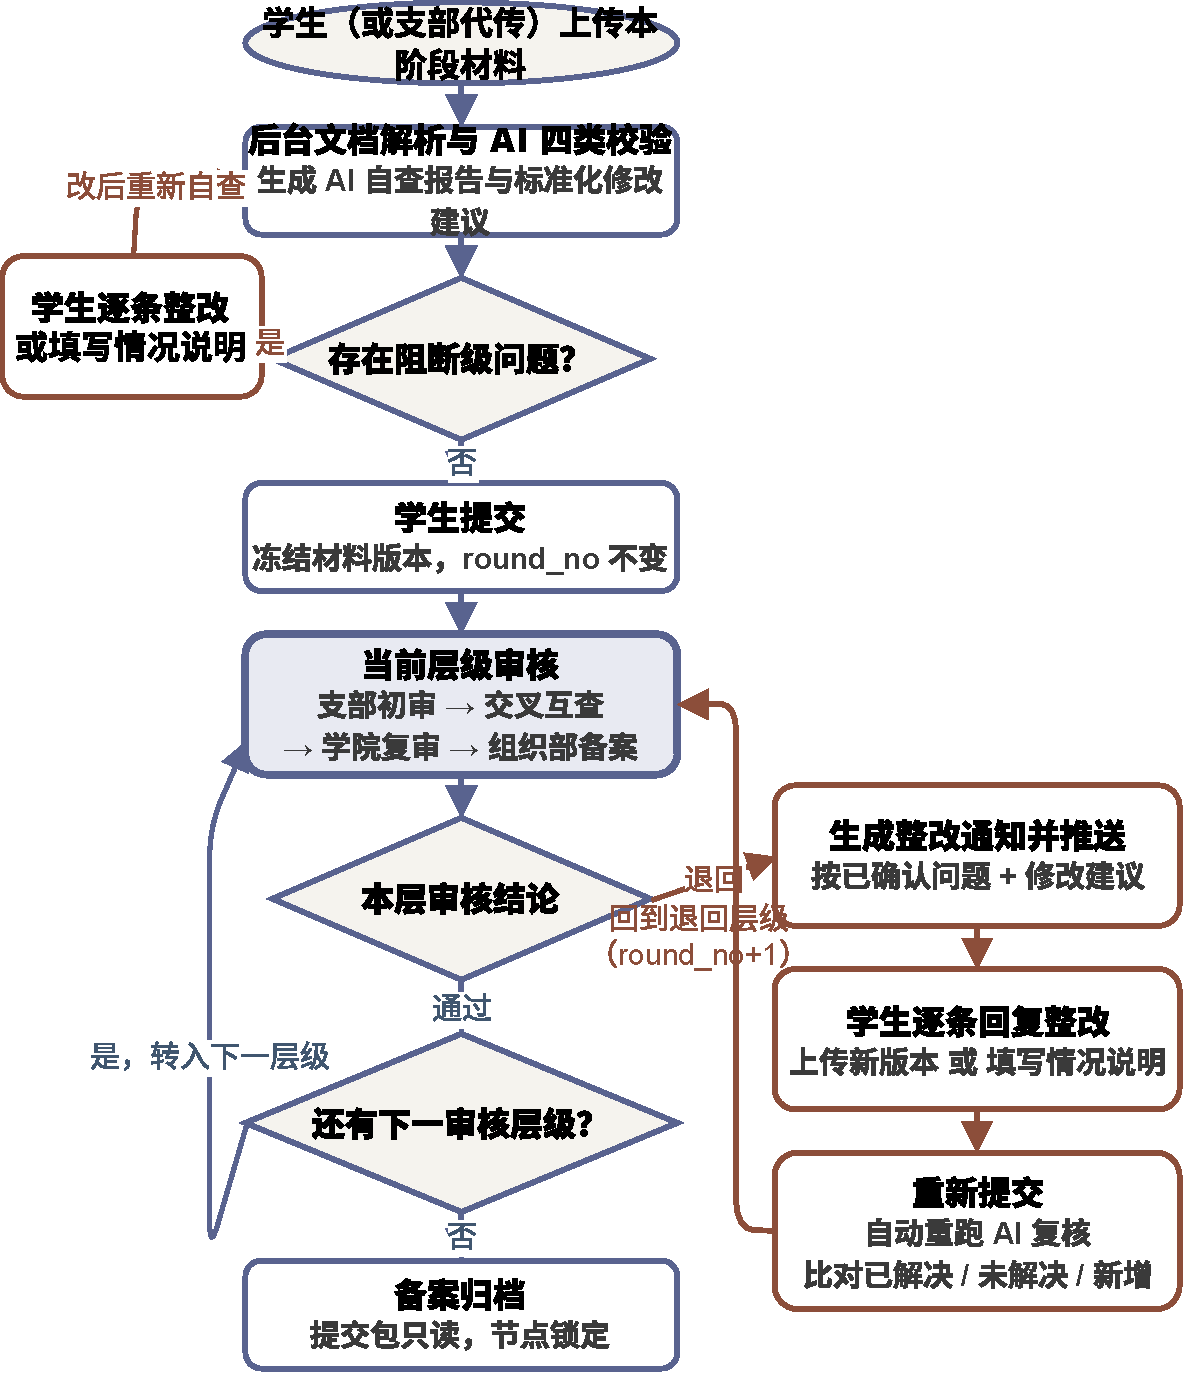
\includegraphics[width=\textwidth,height=0.62\textheight,keepaspectratio]{../figures/fig_flow_1.pdf}
  \caption{提交包审核与整改闭环业务流程}
  \label{fig:flow1}
\end{figure}

图~\ref{fig:flow1} 给出了提交包从上传、AI 校验到多级审核、整改回退的主流程。流程中有两个关键的判断分支：其一，上传材料后系统自动执行文档解析与四类 AI 校验，若存在阻断级问题，学生必须逐条整改或填写情况说明后方可提交；其二，每一级审核员作出"通过/退回"的决定，退回时系统自动生成整改通知并推送给学生，学生逐条回复整改后重新提交，系统自动复核问题是否消除，再回到发起退回的层级，形成闭环。所有退回与重新提交都记录轮次（\texttt{round\_no}），保证整改过程可追溯。

\subsubsection{提交包状态机}

提交包的状态流转规则如表~\ref{tab:state} 所示。状态机是整个审核业务的核心约束：只有处于特定状态、由特定角色发起的操作才被允许，非法流转一律拒绝并记录，这保证了审核程序的严肃性。

\begin{table}[H]
  \centering
  \caption{提交包状态机的主要流转}
  \label{tab:state}
  \footnotesize
  \setlength{\tabcolsep}{4pt}
  \begin{tabular}{p{3.5cm}p{1.7cm}p{2.7cm}p{5.4cm}}
    \toprule
    \textbf{当前状态} & \textbf{动作} & \textbf{执行角色} & \textbf{目标状态} \\
    \midrule
    DRAFT & 提交 & 学生本人（或支部代提交） & BRANCH\_REVIEW \\
    BRANCH\_REVIEW & 通过 & 本支部审核员 & CROSS\_REVIEW（无互查配对时直达 COLLEGE\_REVIEW） \\
    CROSS\_REVIEW & 通过 & 交叉互查审核员 & COLLEGE\_REVIEW \\
    COLLEGE\_REVIEW & 通过 & 学院党委审核员 & ORG\_FILING \\
    ORG\_FILING & 备案 & 组织部管理员 & FILED（档案进入下一阶段） \\
    任一审核态 & 退回 & 当前层级审核员 & RETURNED（记录退回层级与轮次） \\
    RETURNED & 重新提交 & 学生本人 & 回到发起退回的层级 \\
    \bottomrule
  \end{tabular}
\end{table}

\subsection{用户角色与权限需求}

系统不开放注册，账号由管理员开通，首次登录强制修改密码。角色与数据范围需求如表~\ref{tab:role} 所示。权限模型的关键约束有三条：一是数据范围必须按组织层级强制隔离，学生只能访问本人档案，支部审核员只能访问本支部档案，学院审核员只能访问本学院档案，跨范围访问一律返回无权限或不存在；二是"本支部不能互查自己"，交叉互查员与其被审查的支部必须有校验关系；三是多角色用户通过当前激活角色（\texttt{X-Active-Role}）切换视角，避免权限混淆。

\begin{table}[H]
  \centering
  \caption{角色与数据范围}
  \label{tab:role}
  \small
  \begin{tabular}{p{2.6cm}p{4.2cm}p{7.0cm}}
    \toprule
    \textbf{角色} & \textbf{数据范围} & \textbf{主要职责} \\
    \midrule
    发展学生 & 仅本人档案 & 上传/替换本人材料；发起 AI 自查；查看问题清单与修改建议；逐条回复整改；提交审核；查看进度与消息 \\
    党支部审核员 & 本支部 & 代提交、初审待办与审核工作区；发起批量 AI 审核；生成整改通知；批量审核操作 \\
    交叉互查员 & 被分配的支部 & 对指定支部提交包开展交叉互查 \\
    学院党委审核员 & 本学院 & 复审、退回；\allowbreak 本学院统计 \\
    组织部管理员 & 全校 & 备案归档；规则库与系统配置；统计与报表导出；审计日志 \\
    系统管理员 & 全校 & 组织架构、账号管理、系统参数、任务监控 \\
    \bottomrule
  \end{tabular}
\end{table}

\subsection{功能性需求}

按照业务模块划分，系统功能性需求可归纳为八组。

\textbf{（1）账号、权限与审计。} 支持登录登出、连续失败锁定、首登改密、个人中心；所有业务接口按角色与数据范围鉴权；登录、上传、审核、导出、规则变更等关键操作写入审计日志，审计日志不提供删除接口。

\textbf{（2）基础数据管理。} 组织架构（学校—学院—支部）树形管理；用户管理（新增、停用、重置密码、角色授权）；学生与档案的 Excel 批量导入（导入前逐行预校验并返回行号、列与错误原因）；发展批次管理（含各级审核截止日）。

\textbf{（3）档案与材料。} 发展档案建立与查看；阶段进度时间轴；材料上传（PDF、JPG、PNG、DOCX，可留空材料类型交由系统识别）；ZIP 批量上传并按"学号\_材料名"自动归档；材料在线逐页预览；材料版本管理（替换生成新版本，保留历史版本与整改前后对比）。

\textbf{（4）解析与 AI 校验。} 文档解析与扫描件 OCR；解析结果人工校正（时间节点校正必须填写原因）；材料种类识别与份数统计；材料完整性校验与一键生成补全提示；关键时间节点自动提取；时间逻辑、形式规范、内容规范校验；问题自动汇总与分级；标准化修改建议生成；学生 AI 自查；批量 AI 审核；整改后自动复核；AI 结果人工确认（确认/驳回误报/手动新增问题）；AI 审核质量评估；未配置大模型时的规则降级模式。

\textbf{（5）多级审核与整改闭环。} 审核待办与筛选；审核工作区（左侧材料预览、右侧问题清单与审核决定）；支部初审、交叉互查、学院复审、组织部备案；人工接管；批量审核操作；审核记录留痕；整改通知生成与 Word/PDF 导出；学生整改闭环；站内消息通知。

\textbf{（6）规则库。} 材料清单、材料类型、时间节点与时间规则配置；政治术语库与敏感表述库（支持 Excel 导入导出）；修改建议模板库；规则版本记录与追溯。

\textbf{（7）统计与导出。} 工作台首页（按角色显示待办、批次进度、问题分布、高频规则）；审核统计看板（分类、级别、支部、阶段分布与流转趋势）；AI 效能统计；去隐私数据导出与报表导出。

\textbf{（8）系统管理。} AI 服务配置（密钥不回显、连通性测试）；系统参数（上传、留存、通知、AI、OCR、安全、任务线程、工作日历八组）；后台任务监控与重试；演示数据初始化。

\subsection{非功能性需求}

\begin{enumerate}[label=（\arabic*）]
  \item \textbf{可追溯性}：任何一条 AI 问题都必须能追溯到规则依据与原文位置；任何一次审核结论都必须能追溯到审核人、时间与所依据的 AI 报告；报告必须记录生成时使用的规则版本，启用大模型时还须记录实际使用的模型名称。
  \item \textbf{可配置性}：材料清单、时间规则、术语库等业务规则必须由业务人员在界面上配置，不依赖修改代码；规则支持启停与版本化。
  \item \textbf{安全性}：材料文件只能通过鉴权接口读取，存储目录不得对外暴露；密码使用 bcrypt 加盐存储；接口令牌使用 JWT，支持刷新与吊销；敏感配置（如大模型密钥）不回显。
  \item \textbf{可靠性}：文档解析与 AI 审核在后台任务中执行，不阻塞前端操作；任务失败可重试；长耗时任务（如 OCR）异常不得影响主服务。
  \item \textbf{性能}：列表与统计接口在演示数据规模（数十份档案、上百个提交包）下应在一秒内返回；批量审核应支持并发执行。
  \item \textbf{可用性}：界面须适配党务工作人员的使用习惯，待办突出、问题分级清晰、材料原文与问题对照方便；对关键操作给出明确反馈。
\end{enumerate}

\subsection{需求难点分析}

对照榜题提出的四项 AI 需求，需求分析的难点集中在三个方面。第一，\textbf{材料种类识别}需要覆盖打印件扫描、手机拍照、Word 电子稿等多种来源，识别结果必须给出置信度，低置信度时转人工确认；第二，\textbf{时间节点校验}的规则数量多、参数可变（如培养周期、公示时长），且同一节点可能在多份材料中重复出现并互相矛盾，需要设计统一的节点合并与冲突判定策略；第三，\textbf{内容规范核查}中政治术语类问题可以规则化，但意识形态表述类问题只能提示、不能判定，系统必须为此设计"需人工研判"这一中间态，并配套人工接管机制。

\clearpage
\section{系统设计}

\subsection{设计目标与原则}

系统设计遵循四条原则。第一，\textbf{业务规则与代码分离}：材料清单、时间规则、术语库、建议模板全部落库，由界面配置、版本化管理，规则调整不修改代码。第二，\textbf{AI 与人工权责清晰}：AI 只产出建议与问题清单，审核结论由人作出；需要研判的场景由系统强制转人工接管，人工结论覆盖 AI 结论。第三，\textbf{一切可追溯}：审核记录、审计日志、规则版本、材料版本四类留痕机制覆盖全部关键操作。第四，\textbf{后台任务与请求处理解耦}：解析、OCR、批量审核、导出等耗时操作一律异步执行，前端即时得到任务号并轮询进度。

\subsection{总体架构设计}

系统采用前后端分离的五层架构，如图~\ref{fig:arch} 所示。

\begin{figure}[H]
  \centering
  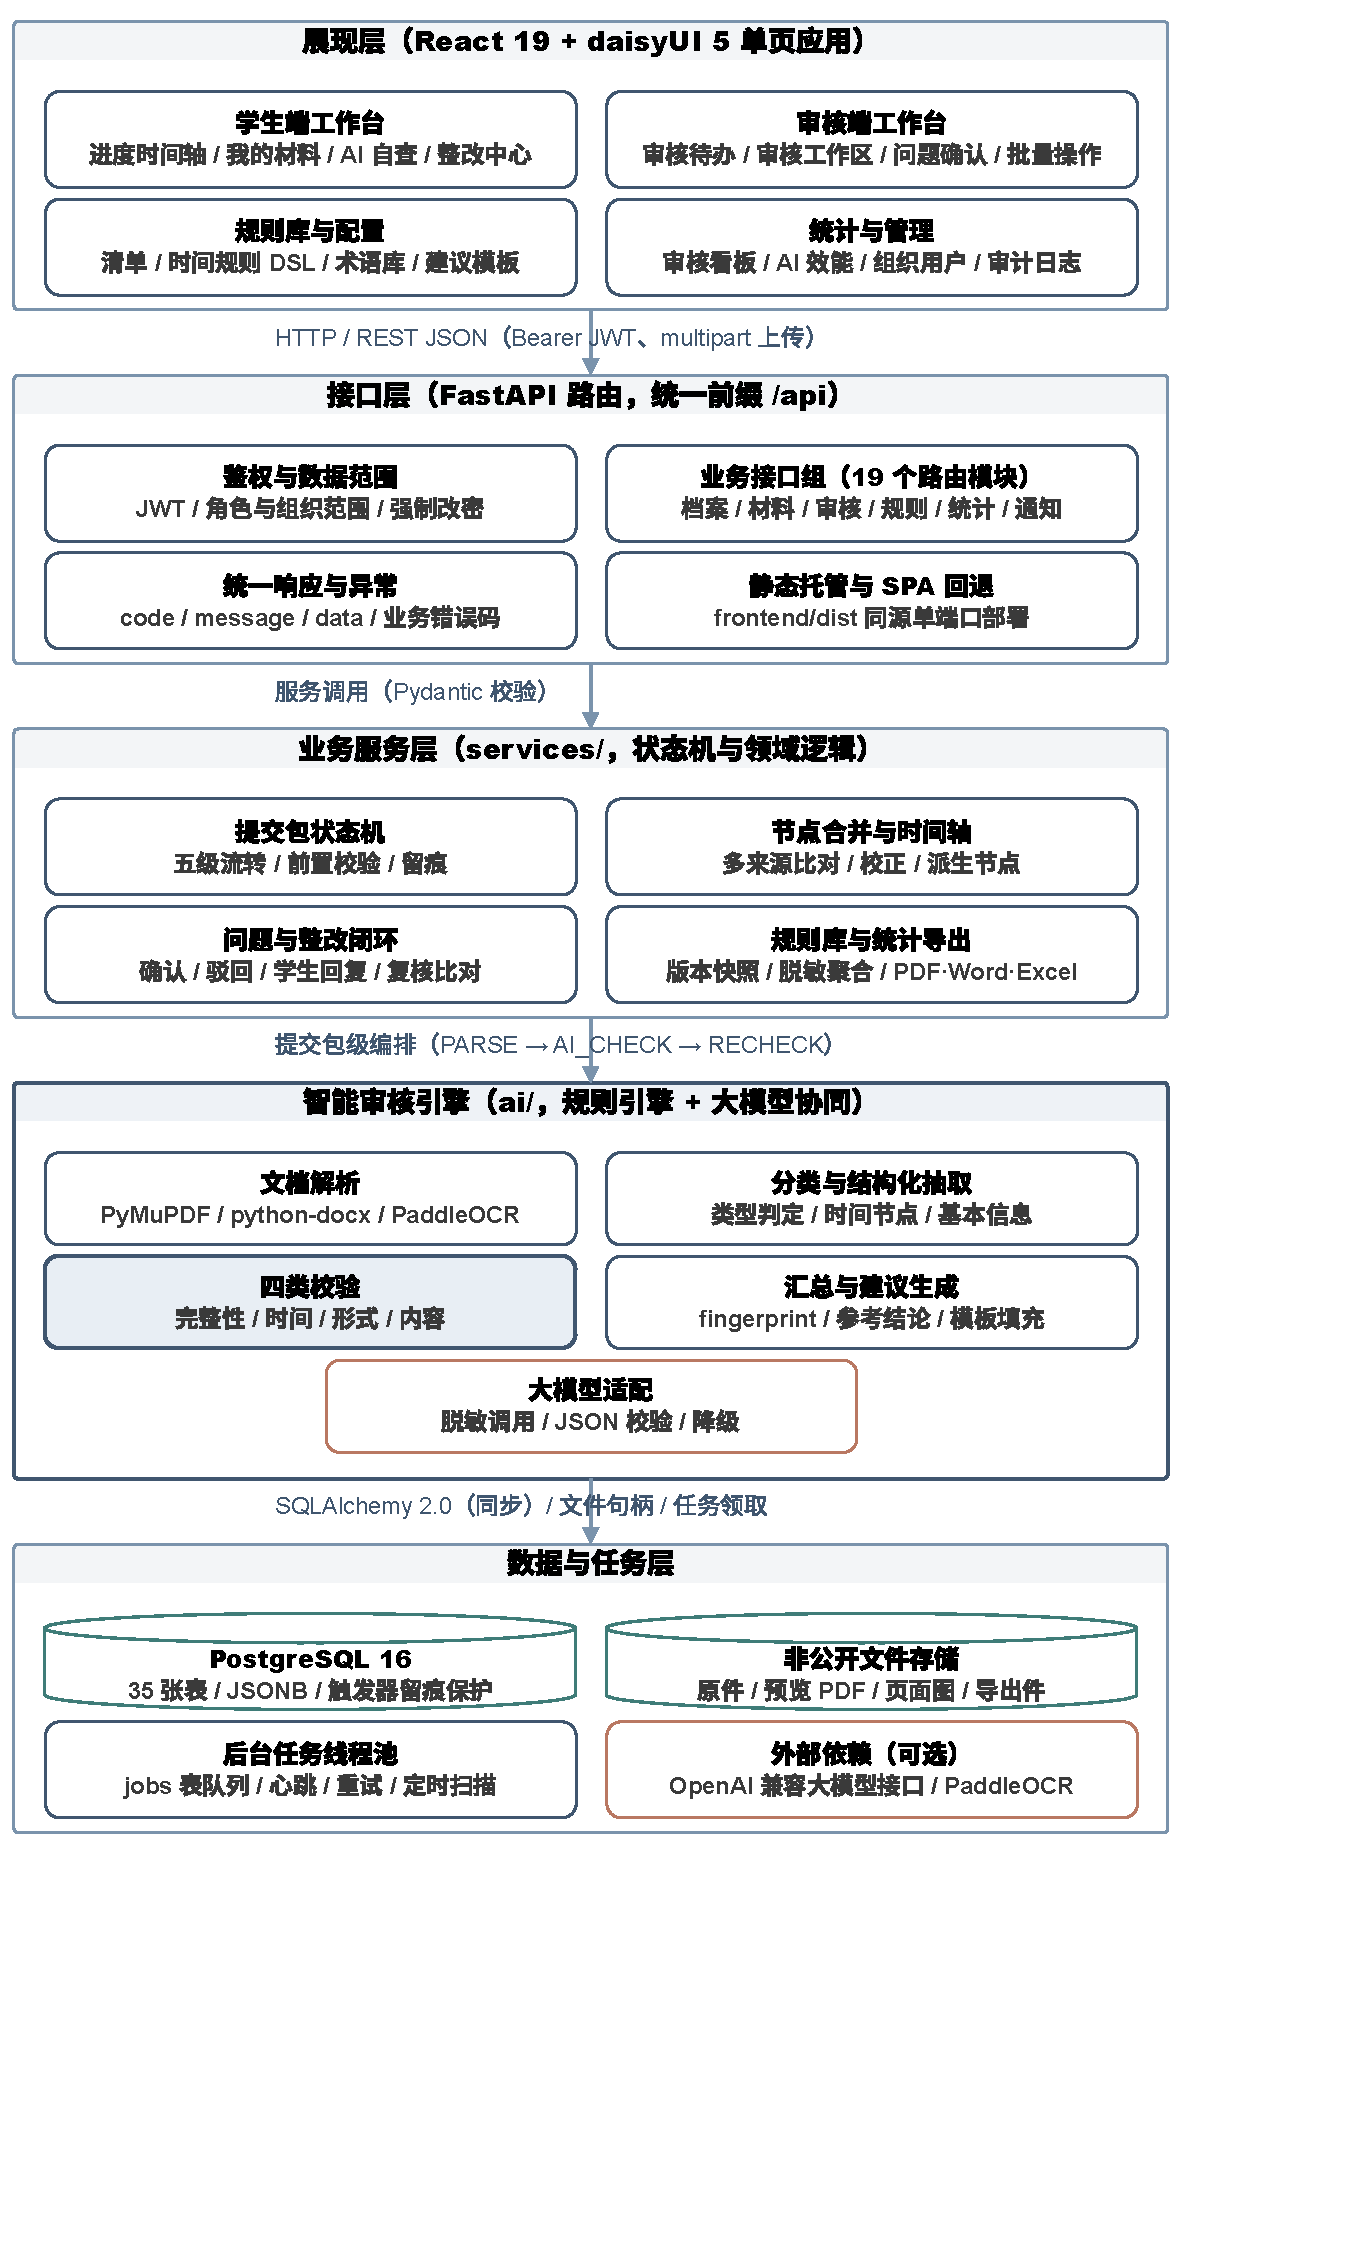
\includegraphics[width=\textwidth]{../figures/fig_arch.pdf}
  \caption{系统总体架构}
  \label{fig:arch}
\end{figure}

\textbf{展现层}为 React 19 单页应用，按角色提供学生端工作台、审核端工作台、规则库与配置、统计与管理四类界面，构建产物由后端同源托管，避免跨域与额外的部署复杂度。\textbf{接口层}基于 FastAPI 构建，按业务域拆分为十九个路由模块，统一响应结构与异常处理，集中完成鉴权、数据范围校验与静态资源托管。\textbf{业务服务层}承载提交包状态机、节点合并与时间轴、问题与整改闭环、规则库与统计导出等核心业务逻辑，是接口层与数据层之间的稳定边界。\textbf{智能审核引擎}独立于业务服务层，内部再分为文档解析、分类与结构化抽取、四类校验、汇总与建议生成四个环节，大模型适配作为可选组件接入，未配置时自动降级为纯规则模式。\textbf{数据与任务层}由 PostgreSQL 数据库、非公开文件存储与后台任务线程池构成，外部依赖（如大模型服务）全部为可选项。

\subsection{数据库设计}

\subsubsection{总体结构}

数据库共设计 35 张表，覆盖用户组织、档案材料、智能审核、审核流转、规则配置、系统管理六个数据域。表~\ref{tab:dbtables} 列出了主要数据表分组，图~\ref{fig:er} 给出了核心实体及其关系（受篇幅限制，图中展示 24 张核心表）。

\begin{table}[H]
  \centering
  \caption{主要数据表分组}
  \label{tab:dbtables}
  \small
  \begin{tabular}{p{2.6cm}p{10.8cm}}
    \toprule
    \textbf{数据域} & \textbf{主要数据表} \\
    \midrule
    组织与用户 & orgs（组织架构，自关联树）、users（账号）、user\_roles（角色授权）、revoked\_tokens（令牌吊销） \\
    档案与材料 & archives（发展档案）、submissions（提交包）、materials（材料）、material\_versions（材料版本）、parse\_results（解析结果） \\
    智能审核 & time\_node\_extractions（节点抽取）、archive\_time\_nodes（档案时间轴）、ai\_reports（AI 报告）、issues（问题） \\
    审核流转 & review\_records（审核记录）、notices（整改通知）、messages（站内消息）、cross\_review\_pairs（互查配对） \\
    规则配置 & checklist\_items、material\_types、time\_node\_defs、time\_rules、check\_rules、political\_terms、sensitive\_phrases、suggestion\_\allowbreak templates、rule\_versions \\
    系统管理 & batches（批次）、jobs（后台任务）、batch\_upload\_items、audit\_logs、system\_settings、export\_files \\
    \bottomrule
  \end{tabular}
\end{table}

核心表按业务域分为三组。图~\ref{fig:er} 为组织、账号与档案材料一组，外键自组织架构逐级指向用户、批次、发展档案、提交包、材料与材料版本；图~\ref{fig:er2} 为时间节点与审核结果一组，节点抽取与档案节点值都引用时间节点定义，审核报告引用提交包与规则版本，问题清单同时指向报告与材料；图~\ref{fig:er3} 为规则配置与运行支撑一组，材料清单引用材料类型，审核留痕、后台任务与站内消息分别引用提交包和用户。图中省略了连线，外键已在各表字段中标出，完整建表语句见数据库脚本。

\begin{figure}[H]
  \centering
  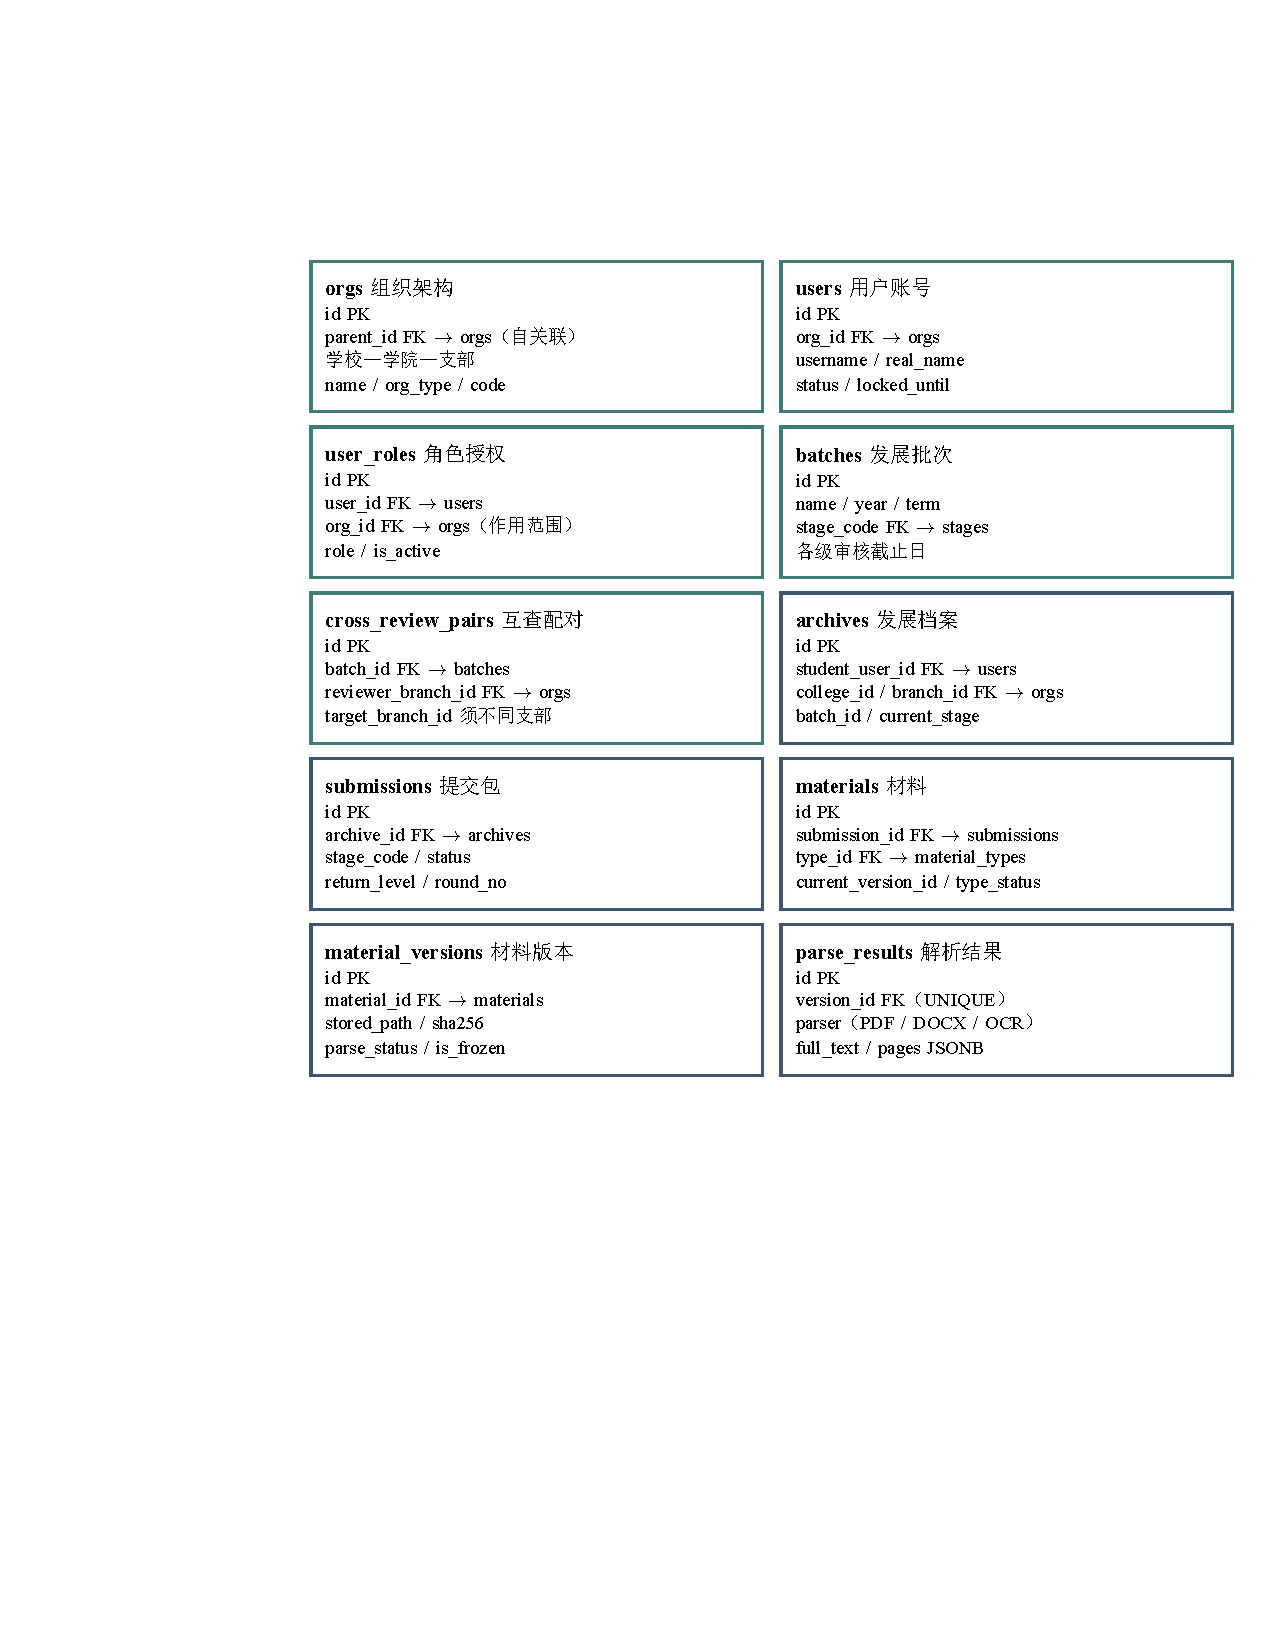
\includegraphics[width=\textwidth]{../figures/fig_er_1.pdf}
  \caption{核心数据表（一）：组织、账号、档案与材料}
  \label{fig:er}
\end{figure}

\begin{figure}[H]
  \centering
  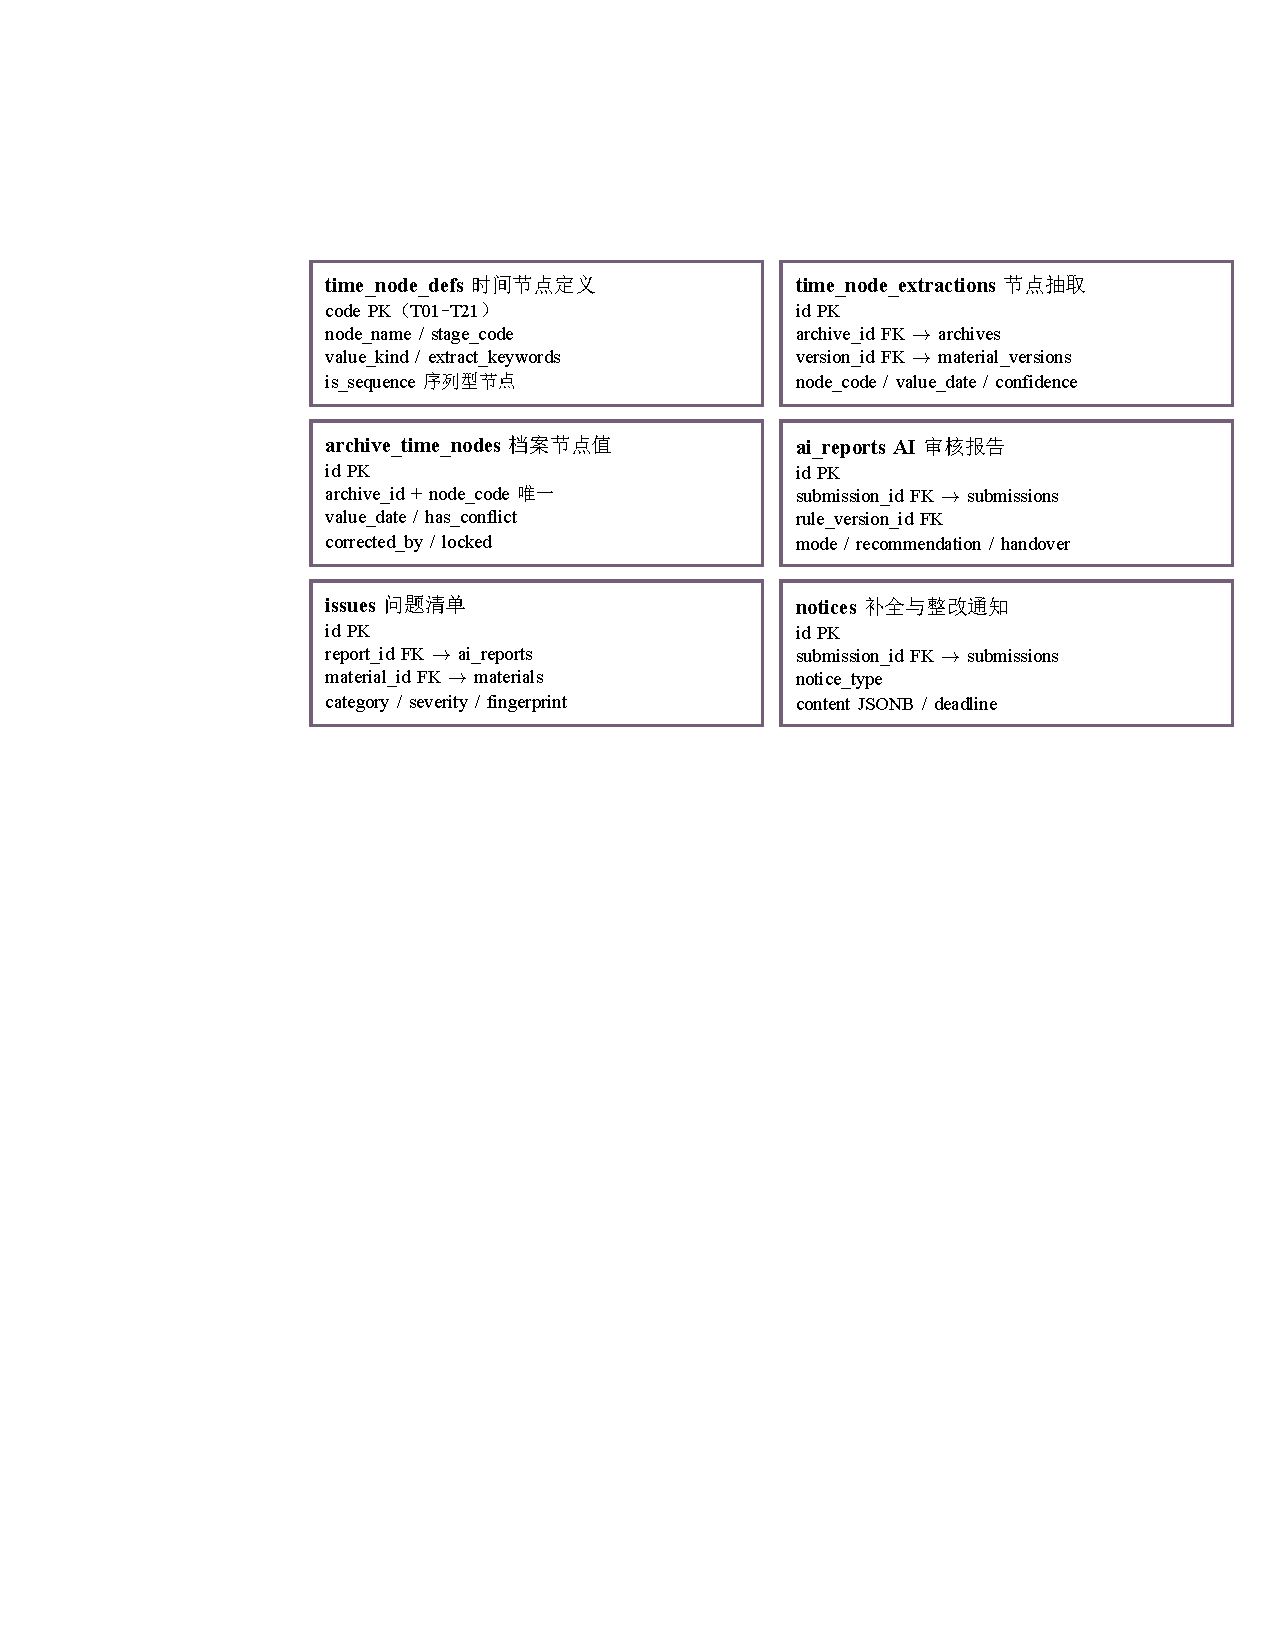
\includegraphics[width=\textwidth]{../figures/fig_er_2.pdf}
  \caption{核心数据表（二）：时间节点与审核结果}
  \label{fig:er2}
\end{figure}

\begin{figure}[H]
  \centering
  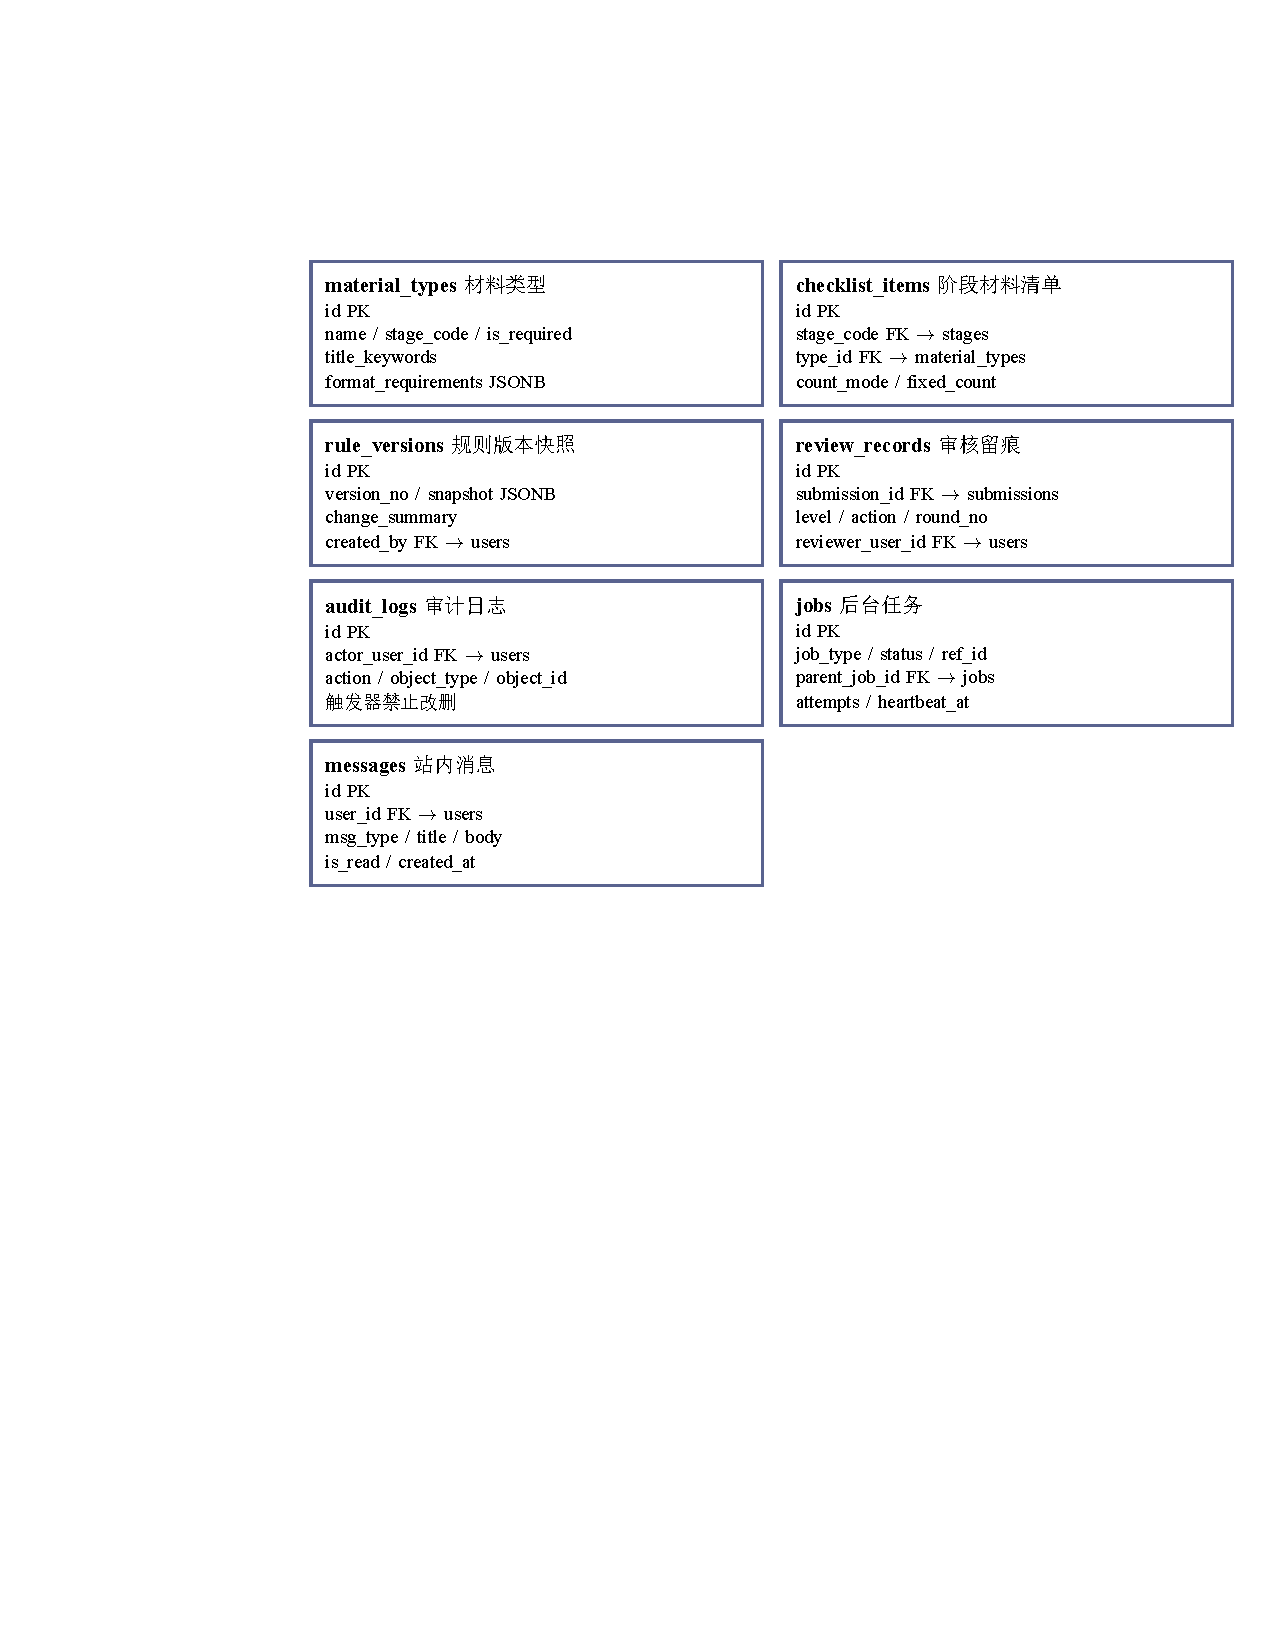
\includegraphics[width=\textwidth]{../figures/fig_er_3.pdf}
  \caption{核心数据表（三）：规则配置、审核留痕与任务}
  \label{fig:er3}
\end{figure}

\subsubsection{关键设计点}

\textbf{（1）以 TEXT + CHECK 表达枚举。} 状态、角色、类别等枚举字段使用文本类型加 CHECK 约束实现，而非数据库原生枚举类型，便于规则调整与数据迁移；所有主键使用 \texttt{BIGINT GENERATED BY DEFAULT AS IDENTITY}。

\textbf{（2）JSONB 承载半结构化数据。} 解析结果、时间轴快照、规则参数、报告明细等结构随业务演进较快，采用 JSONB 存储，既保留查询与索引能力，又避免频繁的加列迁移。

{\sloppy
\textbf{（3）不可篡改性由触发器保证。} \texttt{audit\_\allowbreak logs}、\texttt{review\_\allowbreak records}、\texttt{material\_\allowbreak versions} 三张表建立触发器，禁止 UPDATE 与 DELETE 操作，审计与审核留痕在数据库层面不可篡改；应用层也不提供删除接口。

\textbf{（4）规则版本快照保证可复现。} 任何规则变更都会生成 \texttt{rule\_versions} 记录，AI 报告保存生成时所引用的规则版本号；当规则调整引起结论变化时，可以还原"当时用什么规则得出了什么结论"。

\textbf{（5）材料版本与物理文件分离。} \texttt{materials} 记录材料的逻辑身份；\texttt{material\_\allowbreak versions} 记录每次上传或替换产生的物理文件版本，文件名使用随机标识存储于非公开目录，仅通过鉴权接口读取，整改前后可逐版本对比。
}

\subsection{智能审核引擎设计}

\subsubsection{五阶段流水线}

智能审核引擎是整个系统的核心，设计为"解析—理解—校验—汇总—结论"五个阶段，如图~\ref{fig:flow2} 所示。每个阶段的输出是下一阶段的输入，阶段边界清晰，便于独立测试与降级。

\begin{figure}[H]
  \centering
  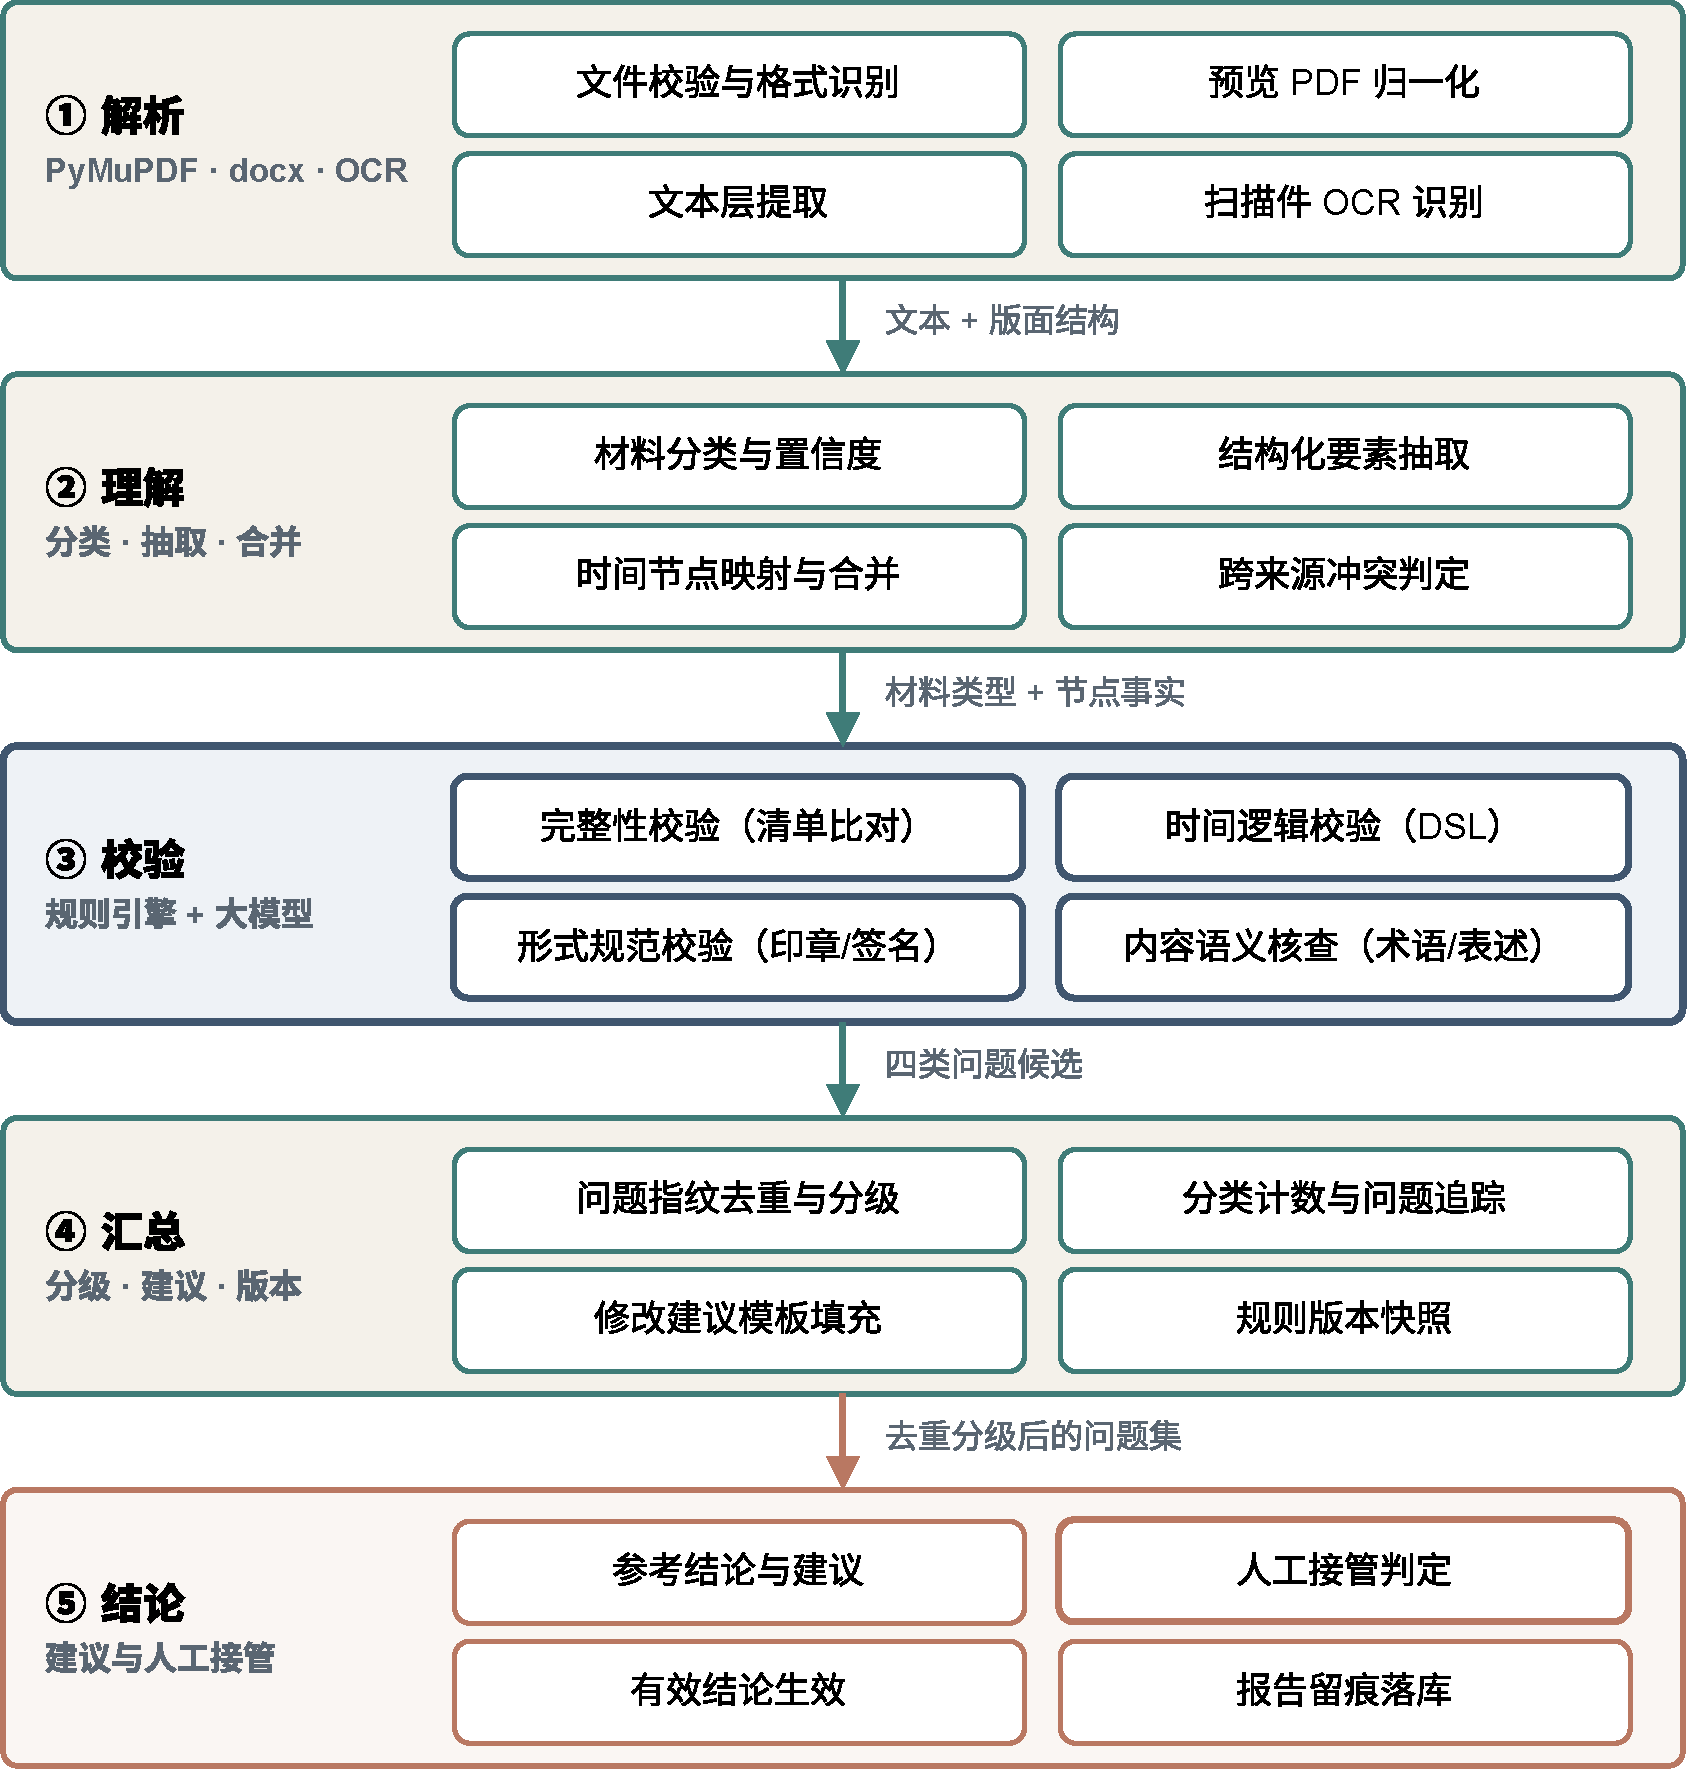
\includegraphics[width=\textwidth,height=0.72\textheight,keepaspectratio]{../figures/fig_flow_2.pdf}
  \caption{智能审核引擎五阶段流水线}
  \label{fig:flow2}
\end{figure}

\textbf{解析阶段}完成文件校验、预览归一化与文本提取：PDF 用 PyMuPDF 提取文本层并逐页渲染为预览图，Word 用 python-docx 提取段落与表格，图片与无文本层的 PDF 走 OCR 适配器；同时检测红色印章等视觉要素。\textbf{理解阶段}基于关键词与结构特征识别材料种类并给出置信度，抽取姓名、日期、落款、党组织名称等结构化要素，再把抽取到的日期映射到统一的时间节点定义（T01--T21）上，同一节点在多个来源出现时按规则合并，数值不一致则标记冲突。\textbf{校验阶段}由规则引擎执行四类检查：完整性检查对照阶段材料清单计算应交与实交份数；时间逻辑检查基于时间规则 DSL 求值；形式规范检查文书结构要素、落款与印章；内容规范检查政治术语、敏感表述与内容要素，其中依赖语义判断的部分调用大语言模型，且只输出"提示"级结论。\textbf{汇总阶段}对问题进行指纹去重、按类别与级别计数、为每条问题填充标准化修改建议，并记录规则版本快照。\textbf{结论阶段}依据问题分布生成"建议通过/建议退回"的参考结论，并判定是否需要人工接管。

\subsubsection{时间规则 DSL}

时间逻辑校验是本系统的特色。系统把时间类要求抽象为一条条时间规则，每条规则由若干算子组合而成，存放在 \texttt{time\_rules} 表中，业务人员可在界面上编辑参数。DSL 共设计 14 个原子算子，表~\ref{tab:dsl} 给出部分算子及其语义。

\begin{table}[H]
  \centering
  \caption{时间规则 DSL 算子（节选）}
  \label{tab:dsl}
  \small
  \begin{tabular}{p{3.0cm}p{5.0cm}p{6.0cm}}
    \toprule
    \textbf{算子} & \textbf{参数} & \textbf{语义} \\
    \midrule
    age\_\allowbreak at\_\allowbreak least & birth, at, years & 在节点 at 时年龄不小于 years 周岁 \\
    before / between & a, b /\allowbreak a, b, c & 日期先后关系与区间约束 \\
    duration\_\allowbreak min & from, to, min & 两节点间隔不小于 min（支持年/月/天） \\
    seq\_\allowbreak period\_\allowbreak count & seq, from, to,\allowbreak period & 序列在区间内应交份数（如思想汇报按季度） \\
    consistent & nodes & 同一节点多来源取值必须一致 \\
    valid\_\allowbreak date & node & 日期合法、要素完整、不晚于上传日 \\
    monotonic & nodes & 阶段主节点严格递增 \\
    derive & name, base, offset & 派生节点（如预备期满日 = 转正预备日 + 1 年） \\
    \bottomrule
  \end{tabular}
\end{table}

以"积极分子培养考察一年以上"（R-T05）为例，其规则定义在数据库中形如：

\begin{lstlisting}
{"rule_code": "R-T05", "category": "TIME", "severity": "BLOCK",
 "params": {"checks": [{"op": "duration_min", "from": "T04",
                        "to": "T08", "min": {"value": 1, "unit": "YEAR"}}]}}
\end{lstlisting}

引擎按算子逐个求值，任一算子失败即生成一条带规则编号、严重级别、涉及节点与原文位置的问题；节点缺失时生成"无法校验"的低级别提示而非误报阻断。

\subsubsection{大模型适配与降级}

需要理解语义的检查（如入党动机表述是否恰当、内容要素是否完整）通过大模型适配层实现。适配层统一封装调用参数、超时、重试与结果解析，并在调用前对个人敏感信息做脱敏处理。语义核查使用内置的内容核查提示词模板：入参为待查规则与材料全文，出参为规则编号、原文片段、理由与置信度；模型结论一律标记为"需人工研判"，只作提示，不直接形成阻断结论，从而与人工接管机制衔接。

系统默认关闭大模型：未配置接口时，报告标记为纯规则模式（RULE\_ONLY），三条语义规则（政治表述准确性、经历与时间线吻合、思想认识深度）在规则结果中记为"跳过"并注明原因，其余功能不受影响。配置接口后，报告标记为规则加模型模式（RULE\_LLM），并记录实际使用的模型名称，保证报告可追溯。为避免外部服务异常拖垮审核流程，语义调用只尝试一次，且同一份报告在首次失败后不再重复调用，失败规则降级为"跳过"并在报告中保留失败原因，检查任务照常完成。这一设计保证了系统在"材料不出校"的约束下仍可完整运行。

\subsubsection{人工接管机制}

人工接管是"AI 不替代人工判断"原则的制度化落地。当报告出现下列情形之一时，系统将报告标记为需要接管（\texttt{handover\_status=REQUIRED}）：存在低置信度识别结果、同一时间节点多来源冲突、问题被标记为需人工研判、以及处于关键阶段的提交包。需要接管的提交包，审核员必须先完成接管（写明接管原因与人工结论），才能执行"通过"或"备案"操作；否则接口返回状态冲突错误。学生的提交与审核员的退回不受此限制，保证整改路径始终通畅。人工结论以"有效结论"（\texttt{effective\_recommendation}）的形式覆盖 AI 建议，两者在报告中同时保留，形成对照。

\subsection{后台任务设计}

文档解析、OCR、AI 审核、批量审核、批量上传归档、通知批量生成、报表导出七类操作耗时较长，全部设计为后台任务。任务表 \texttt{jobs} 记录任务类型、状态、进度、心跳时间、重试次数与父子关系；后台工作线程通过"跳过已锁定行"的取任务方式并发领取任务，支持一个批次拆分为多个子任务并行执行，父任务在所有子任务完成后收尾。任务失败自动重试并记录错误信息，管理界面可查看任务状态并手动重试。

\subsection{安全设计}

\textbf{（1）认证与令牌。} 登录成功后签发有效期 120 分钟的访问令牌与 7 天的刷新令牌，采用 HS256 签名；登出或改密时令牌写入吊销表即时失效；连续失败 5 次锁定账号 15 分钟。

\textbf{（2）授权与数据范围。} 每个用户可拥有多个角色，每个角色绑定一个组织锚点；请求携带当前激活角色，服务端据此限定数据范围，越权访问返回无权限或不存在，不泄露数据是否存在。

\textbf{（3）文件安全。} 材料文件存放于非公开目录，文件名随机化；下载与预览必须携带有效令牌并通过数据范围校验；存储目录不配置为静态目录。系统自测专门验证了直接访问存储目录不会泄露文件。

\textbf{（4）配置安全。} 大模型等外部服务的密钥仅存于服务端配置，接口只返回"是否已配置"的布尔值，不回显明文。

\clearpage
\section{系统实现}

\subsection{开发环境与技术选型}

系统开发与运行环境如表~\ref{tab:env} 所示。技术选型上，后端选择 FastAPI 而非传统企业框架，是因为其类型注解驱动的请求校验与自动生成的接口文档显著降低了前后端联调成本；数据库选择 PostgreSQL 而非 MySQL，是为了使用 JSONB、部分索引与行级锁等特性支撑规则配置与后台任务的并发控制。

\begin{table}[H]
  \centering
  \caption{开发环境与主要技术栈}
  \label{tab:env}
  \small
  \begin{tabular}{p{2.8cm}p{10.6cm}}
    \toprule
    \textbf{类别} & \textbf{技术与版本} \\
    \midrule
    操作系统 / 运行时 & Windows 11；Python 3.13.12；Node.js 24 \\
    前端 & React 19.3 + React Router 7.18 + Vite 8.3 + Tailwind CSS 4.3 + daisyUI 5.7（nord 主题）+ Recharts 3.10 + axios + dayjs \\
    后端 & FastAPI 0.139 + Uvicorn 0.30 + SQLAlchemy 2.0（同步）+ Pydantic 2.13 + psycopg 3.3 \\
    数据库 & PostgreSQL 16.15（35 张业务表） \\
    文档处理 & PyMuPDF 1.27（PDF 解析与逐页渲染）、python-docx 1.2（Word 解析）、OpenCV（印章等视觉要素检测）、PaddleOCR 3.5（扫描件 OCR，可选依赖） \\
    安全 & bcrypt 4.0（口令散列）、PyJWT 2.15（JWT 签发与校验）、cryptography（Fernet 加密敏感配置） \\
    \bottomrule
  \end{tabular}
\end{table}

\subsection{后端实现}

\subsubsection{接口层与统一约定}

后端入口为 \texttt{code/backend/main.py}，按业务域拆分为十九个路由模块（认证、组织、用户、批次、档案、提交包、材料、解析、AI 报告、问题、审核、整改通知、消息、规则、统计、导出、任务、设置、健康检查）。所有接口统一返回 \texttt{\{code, message, data\}} 结构：成功时 \texttt{code=0}，业务错误返回非零业务码并配合合适的 HTTP 状态，例如参数错误 40000/400、未登录 40100/401、越权 40300/403、状态冲突 40900/409、校验失败 42200/422、账号锁定 42300/423。异常处理中间件统一兜底，内部错误只返回 50000，不向前端泄露堆栈。

鉴权采用依赖注入实现：受保护接口统一声明当前用户依赖，解析 JWT、校验令牌是否被吊销、加载用户角色，再从请求头读取当前激活角色并构造数据范围对象。数据范围判定集中在 \texttt{services/scope.py}，业务代码只通过该对象取数，避免范围条件散落在各处造成越权。

\subsubsection{业务服务层}

业务逻辑按领域拆分为约二十个服务模块，其中提交包流转（状态机）、时间轴与节点合并、问题与整改闭环、规则库与版本管理是四个核心。状态机的实现方式是：为每个（状态，动作）组合声明守卫条件与目标状态，执行动作时先校验角色与数据范围，再校验守卫条件，全部通过后在一个事务内更新提交包状态、写入审核记录与审计日志、生成下游通知。以支部初审通过为例，守卫条件包括：本层不存在待处理的阻断级问题；AI 报告需要人工接管时已接管完成；报告的有效结论不为空。任一条件不满足即返回对应的冲突码，前端据此提示审核员。同类守卫也用于整改回路：学生回复整改或上传新版本时，系统校验所关联的问题与材料版本必须属于当前提交包及对应材料，跨材料关联一律拒绝并在写入文件前完成校验，保证整改证据与问题一一对应。

\subsubsection{数据访问与并发控制}

后台任务采用"取任务—执行—回写"的模式，多个工作线程并发领取任务时使用跳过锁定行的方式，避免任务重复执行。批量审核的父任务收尾是并发正确性的关键点：多个子任务可能由不同线程完成，父任务必须等待全部子任务结束后才能置为完成。初版实现中子任务完成后直接统计兄弟任务状态，由于事务隔离，两个线程可能都读不到对方尚未提交的状态，导致父任务永远停留在运行中。修复方式是在统计前对父任务行加锁：

\begin{lstlisting}
-- worker.py 父任务收尾（修复后）
SELECT ... FROM jobs WHERE id = :parent_id
FOR NO KEY UPDATE;          -- 阻塞并发收尾，且不与子任务外键的 KEY SHARE 锁冲突
-- 在持锁事务内统计子任务状态，全部终态时更新父任务
\end{lstlisting}

需要说明的是，第一版使用 \texttt{FOR UPDATE} 强锁父任务行，与子任务外键持有的 KEY SHARE 锁相互冲突，在并发压测中触发了大量死锁，数据库日志记录到 58 次死锁；改用 \texttt{FOR NO KEY UPDATE} 后既保证了互斥，又不与键共享锁冲突。修复后 60 个并发批次全部正常收尾，无死锁、无后台错误。

\subsubsection{规则库与版本化}

规则库包含材料清单、材料类型、时间节点定义、时间规则、内容检查规则、政治术语库、敏感表述库与修改建议模板八类配置。所有规则写操作统一经过规则服务的四个公共函数（新增、更新、删除、导入），每个函数在写入规则的同时生成规则版本记录并写入审计日志，保证"规则变更必有版本、必有操作人"。AI 报告保存生成时引用的规则版本号，实现"结论可复现"。

\subsection{智能审核引擎实现}

\subsubsection{文档解析与 OCR}

解析流程按材料格式分流：PDF 用 PyMuPDF 提取文本层，同时逐页渲染为预览图供前端在线预览；Word 用 python-docx 抽取段落与表格文本；图片与无文本层的 PDF 进入 OCR 分支。解析结果（全文、分段文本、页面尺寸、文本位置）统一写入解析结果表，供后续要素抽取与问题定位使用。

OCR 的工程化是本项目的难点之一。PaddleOCR 3.x 与 2.x 的初始化接口不兼容，早期代码按 2.x 编写，在本机 3.5 版本上初始化直接抛异常，随后被静默降级为"未启用 OCR"，导致扫描件实际不可用。修复分两层：其一是按版本适配接口，优先使用 3.x 的预测接口与结果字段，并关闭会抛异常的加速开关，初始化失败时回退 2.x 写法；其二是进程隔离——在服务进程内加载 Paddle 模型会使整个服务进程异常退出且没有回溯，同样的代码在普通脚本中运行正常，判断为原生运行时与 ASGI 服务进程的兼容性问题，因此把 OCR 放到独立的子进程中执行，子进程异常只影响当次识别，服务本身不受影响，服务停止时同步关闭子进程。修复后学生上传扫描件，后台约 36 秒完成解析，正确识别出全文并抽取到落款日期。

\subsubsection{材料分类与要素抽取}

材料分类综合文件名、关键词命中与结构特征给出候选类型与置信度；置信度低于阈值时标记为"待人工确认"，不计入硬性缺失判定。要素抽取同时使用正则与规则模板：日期、姓名、组织名称等强模式要素用正则表达式抽取；"落款—印章—签名"等版面要素结合文本位置与视觉检测结果判定。抽取到的日期按其语义映射到统一的时间节点编码，同一节点有多个来源时按"以正式文书优先、以最新版本优先"的次序合并，取值不一致则保留全部候选并标记冲突。

OCR 输出的文本常含全角数字（如"2０2５年３月１日"），会直接导致日期抽取失败。实现中对全角数字与全角分隔符做一对一替换后再匹配，替换不改变字符位置，因此问题定位的原文偏移不受影响；该场景补充了专门的单元测试。

\subsubsection{四类校验与汇总}

完整性校验按阶段清单计算应交份数：固定份数项直接比对；周期性材料（如思想汇报）按培养周期与季度切分计算应交数量，末段不足配置天数不计。时间校验由 DSL 引擎按算子求值；形式校验检查文书结构要素、落款与印章（印章检测基于颜色与形状的启发式方法）；内容校验先做术语与敏感表述的规则匹配，需要语义判断的部分由大模型按内容核查模板完成，模型返回的每条结果映射为规则编号、原文片段与理由，统一输出"提示"级结论并标注"需人工研判"，因而必然触发人工接管；模型不可用时该规则记为"跳过"并保留失败原因，不影响其余检查。校验产生的问题按指纹去重（规则号 + 节点 + 材料 + 位置），按类别（完整性/时间/形式/内容）与级别（阻断/警告/提示）计数，并为每条问题从模板库填充修改建议，最后写入报告。

\subsection{前端实现}

前端为单页应用，路由按角色分区：学生端包含工作台、我的档案、阶段进度、我的材料、AI 自查、整改中心；审核端包含待办、审核工作区、批量操作；管理与统计侧包含组织、用户、批次、规则库、统计看板、任务监控、审计日志与系统设置。页面通过统一的请求封装携带令牌与激活角色，401 时自动尝试刷新令牌，40301 时强制跳转改密页。

审核工作区是交互最复杂的页面：左侧为材料逐页预览与解析文本对照，右侧为问题清单与审核决定面板；问题按级别排序并支持"确认、驳回误报、手动新增"，选中问题时预览区自动定位到对应页面与文本位置。审核决定提交前，前端先做一层与后端一致的守卫校验（是否存在未处理阻断问题、是否需要人工接管），减少无效请求。

\subsection{界面实现}

图~\ref{fig:ui-login} 至图~\ref{fig:ui-audit} 共 13 张实拍截图（1440$\times$900 视口）展示了系统各主要界面。

登录页如图~\ref{fig:ui-login} 所示，账号由管理员统一开通，不开放自助注册；连续输错密码达到阈值后账号被临时锁定，首次登录会被强制引导至修改密码页面。

\begin{figure}[H]
  \centering
  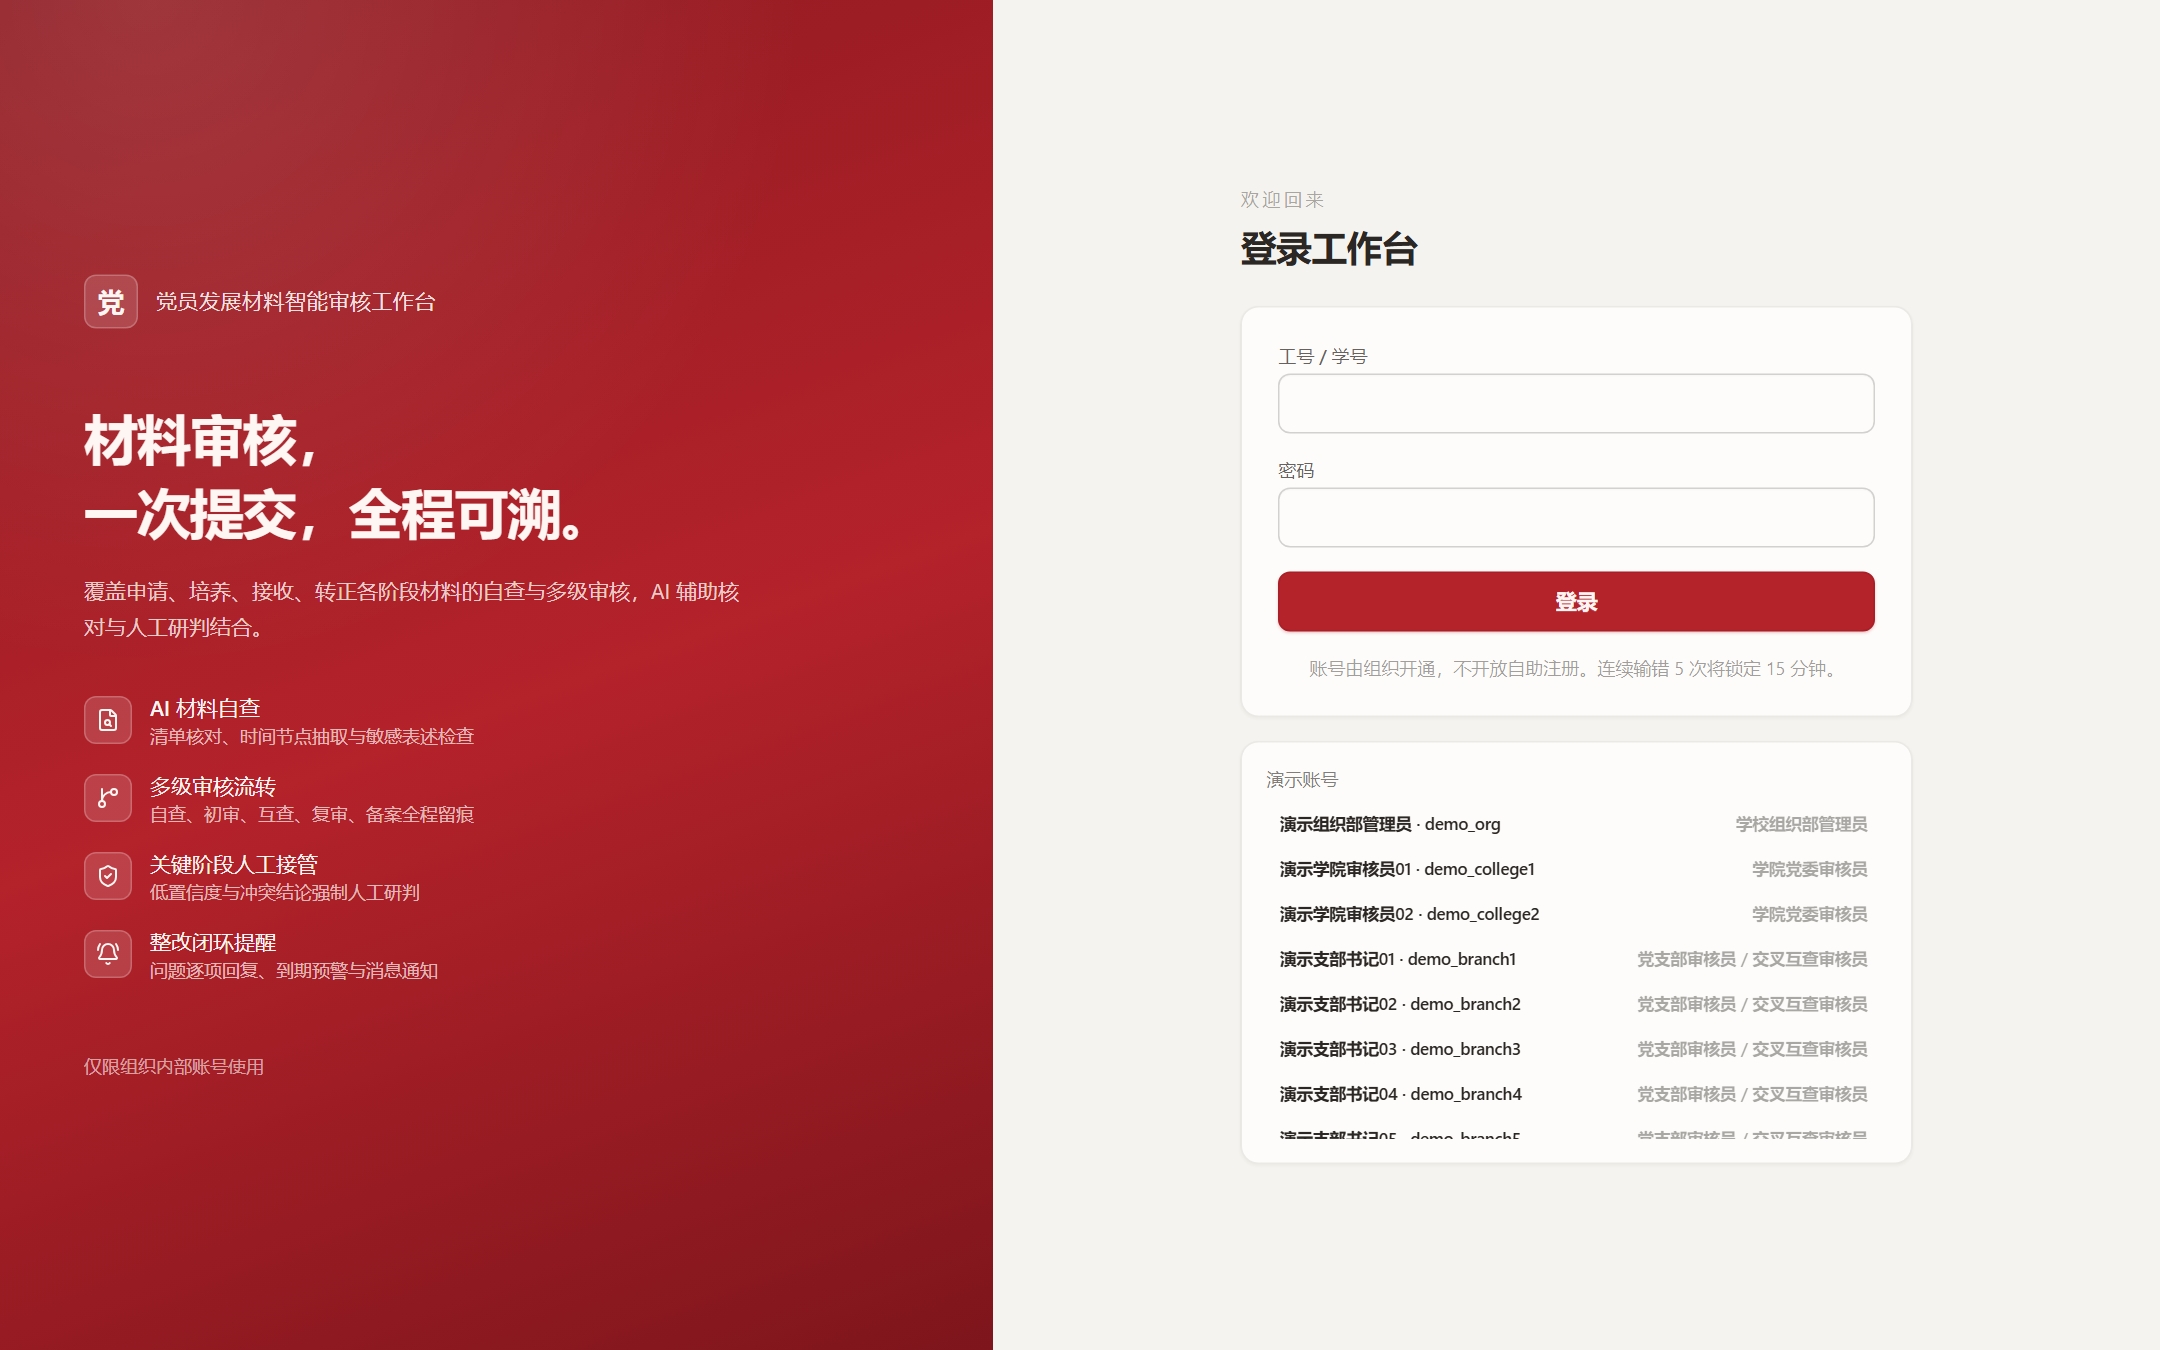
\includegraphics[width=0.72\textwidth]{../figures/shot_login.png}
  \caption{登录页}
  \label{fig:ui-login}
\end{figure}

登录后的工作台按角色呈现不同的待办内容。图~\ref{fig:ui-dash-branch} 是党支部审核员的工作台，突出本支部待初审的提交包数量、当前批次进度与近期问题分布；图~\ref{fig:ui-dash-org} 是组织部管理员的工作台，视角扩大到全校，汇总各学院的备案进度与整体问题构成，便于组织部掌握全校党员发展材料审核的总体情况。

\begin{figure}[H]
  \centering
  \begin{minipage}{0.48\textwidth}
    \centering
    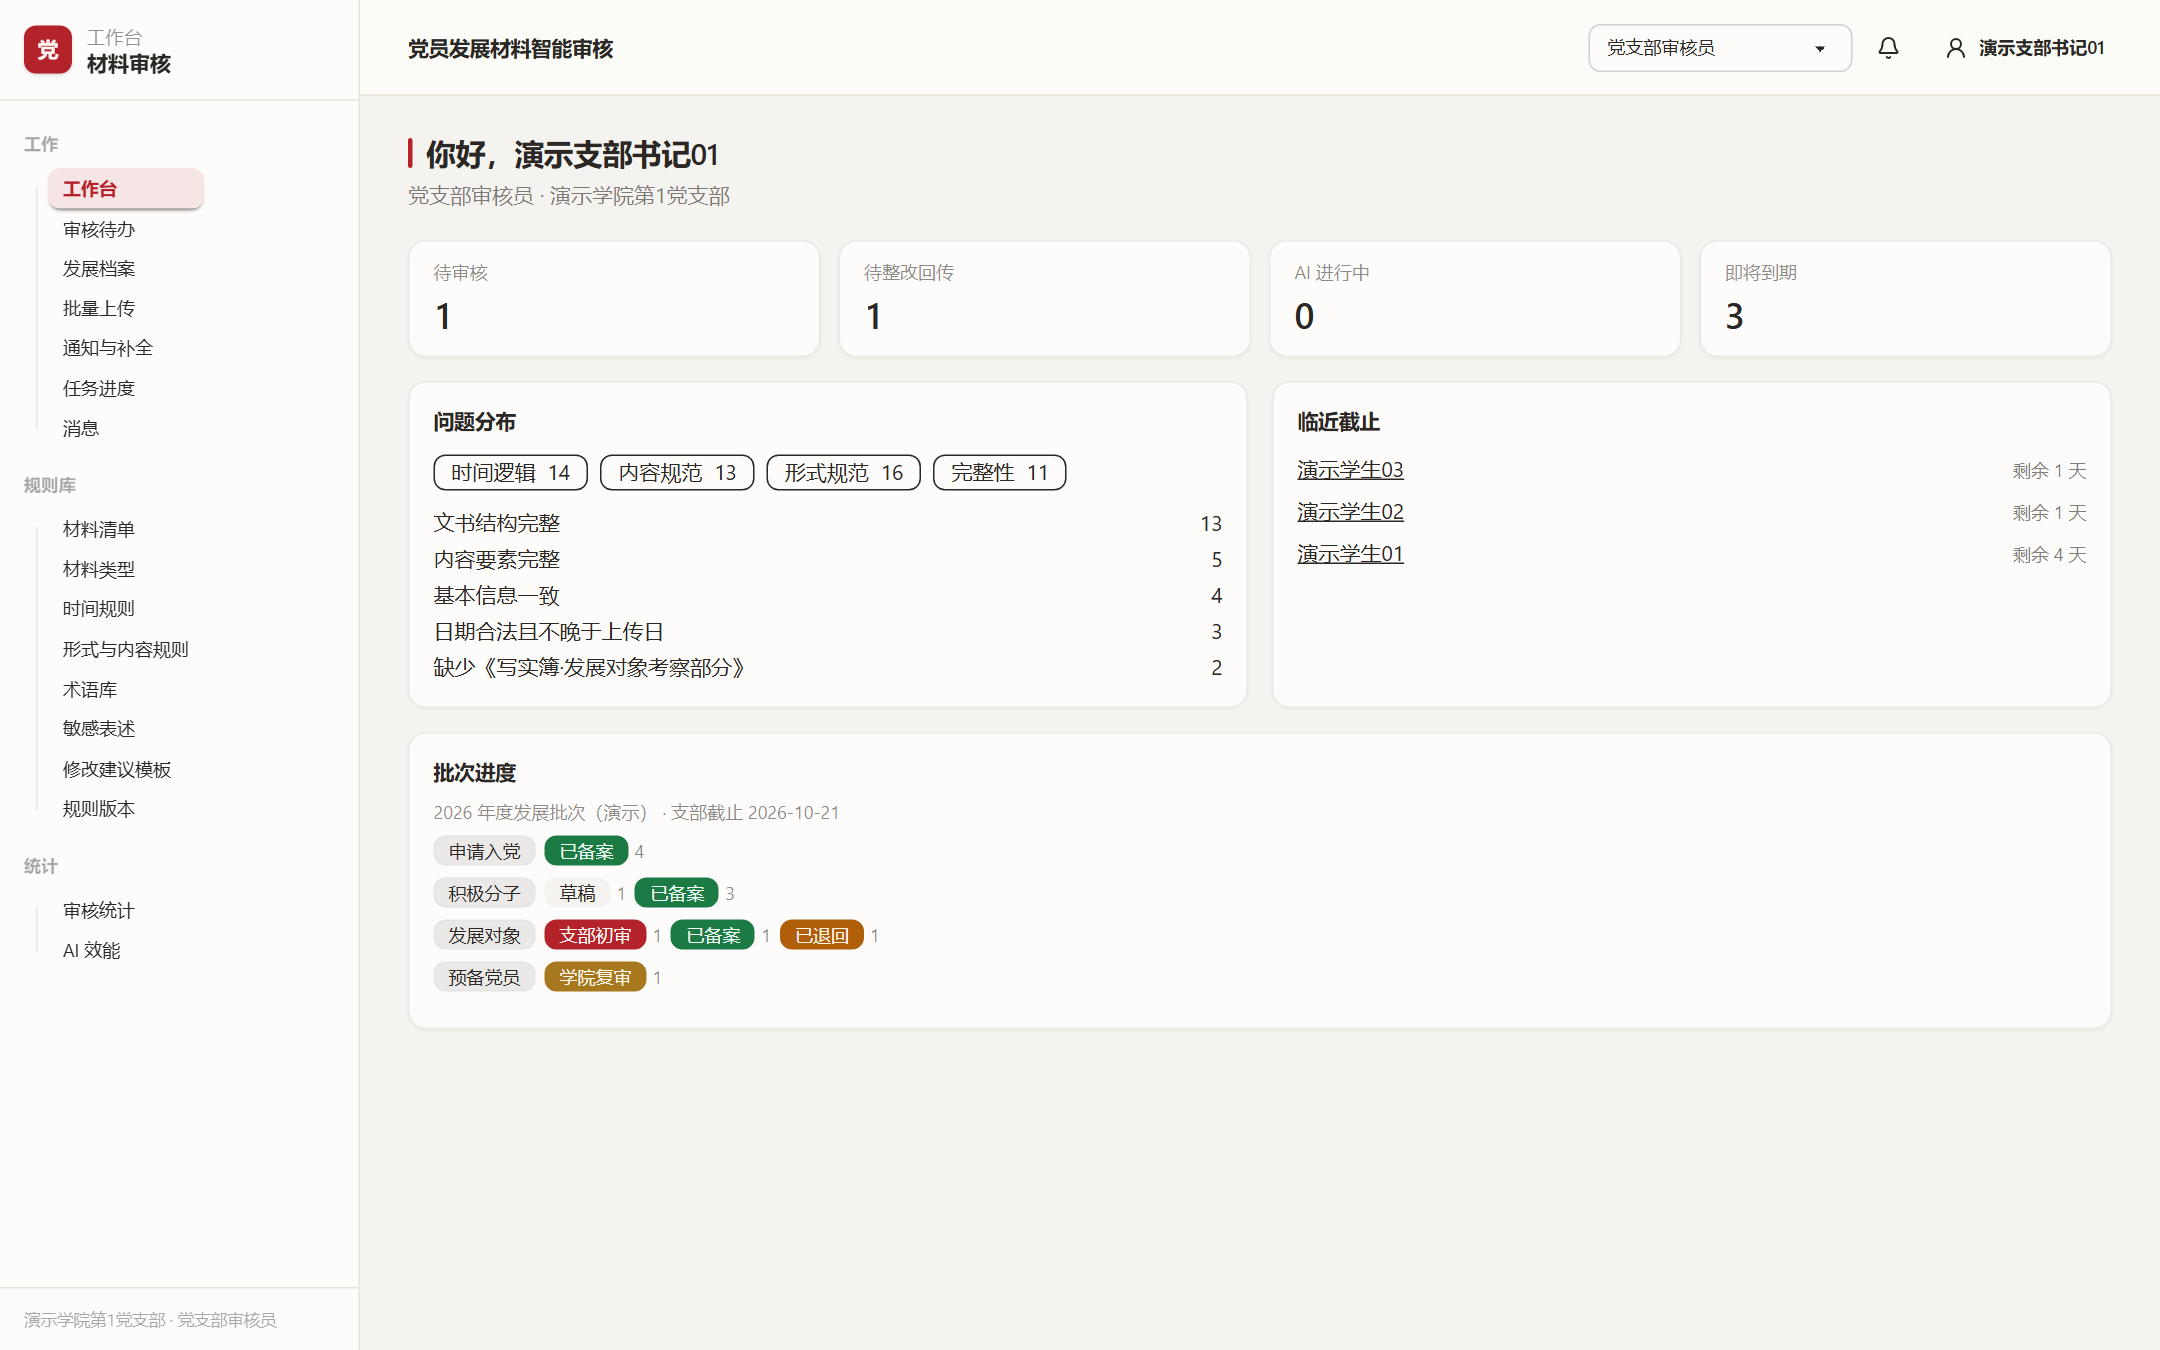
\includegraphics[width=\textwidth]{../figures/shot_dashboard_branch.png}
    \caption{党支部工作台}
    \label{fig:ui-dash-branch}
  \end{minipage}\hfill
  \begin{minipage}{0.48\textwidth}
    \centering
    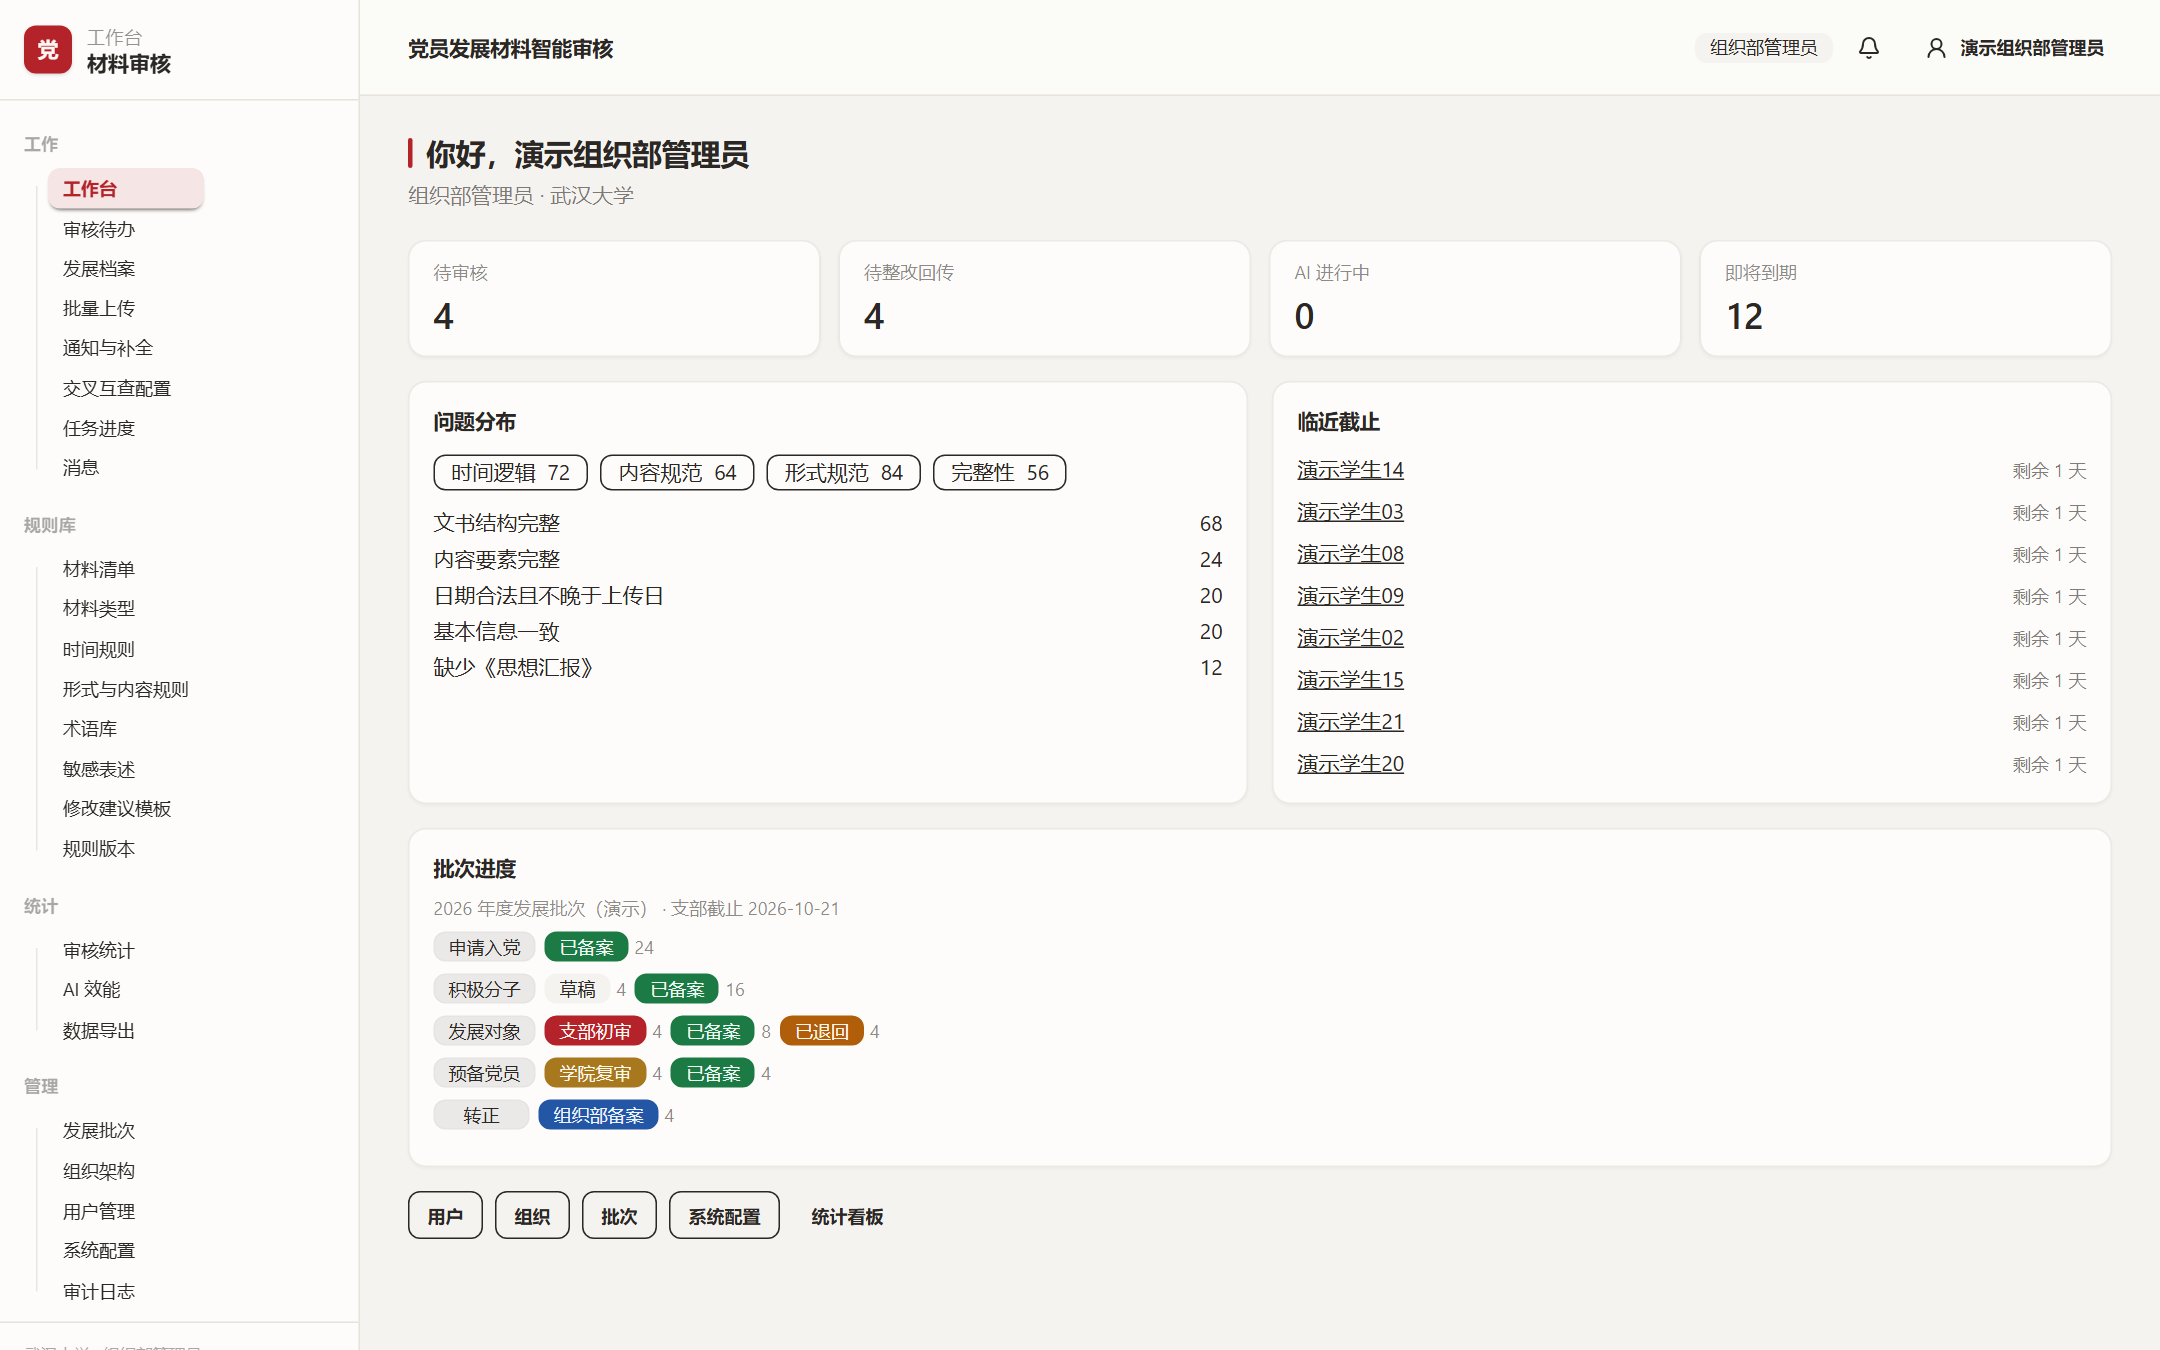
\includegraphics[width=\textwidth]{../figures/shot_dashboard_org.png}
    \caption{组织部工作台}
    \label{fig:ui-dash-org}
  \end{minipage}
\end{figure}

学生端以时间轴呈现个人培养进度。图~\ref{fig:ui-progress} 列出本阶段的关键时间节点及其完成状态，已锁定的历史节点以只读方式展示；图~\ref{fig:ui-materials} 是材料管理页，学生可按材料类型上传、替换与预览文件，系统自动识别材料种类并标注缺失项，替换后的文件保留历史版本，便于与整改前的内容对照。

\begin{figure}[H]
  \centering
  \begin{minipage}{0.48\textwidth}
    \centering
    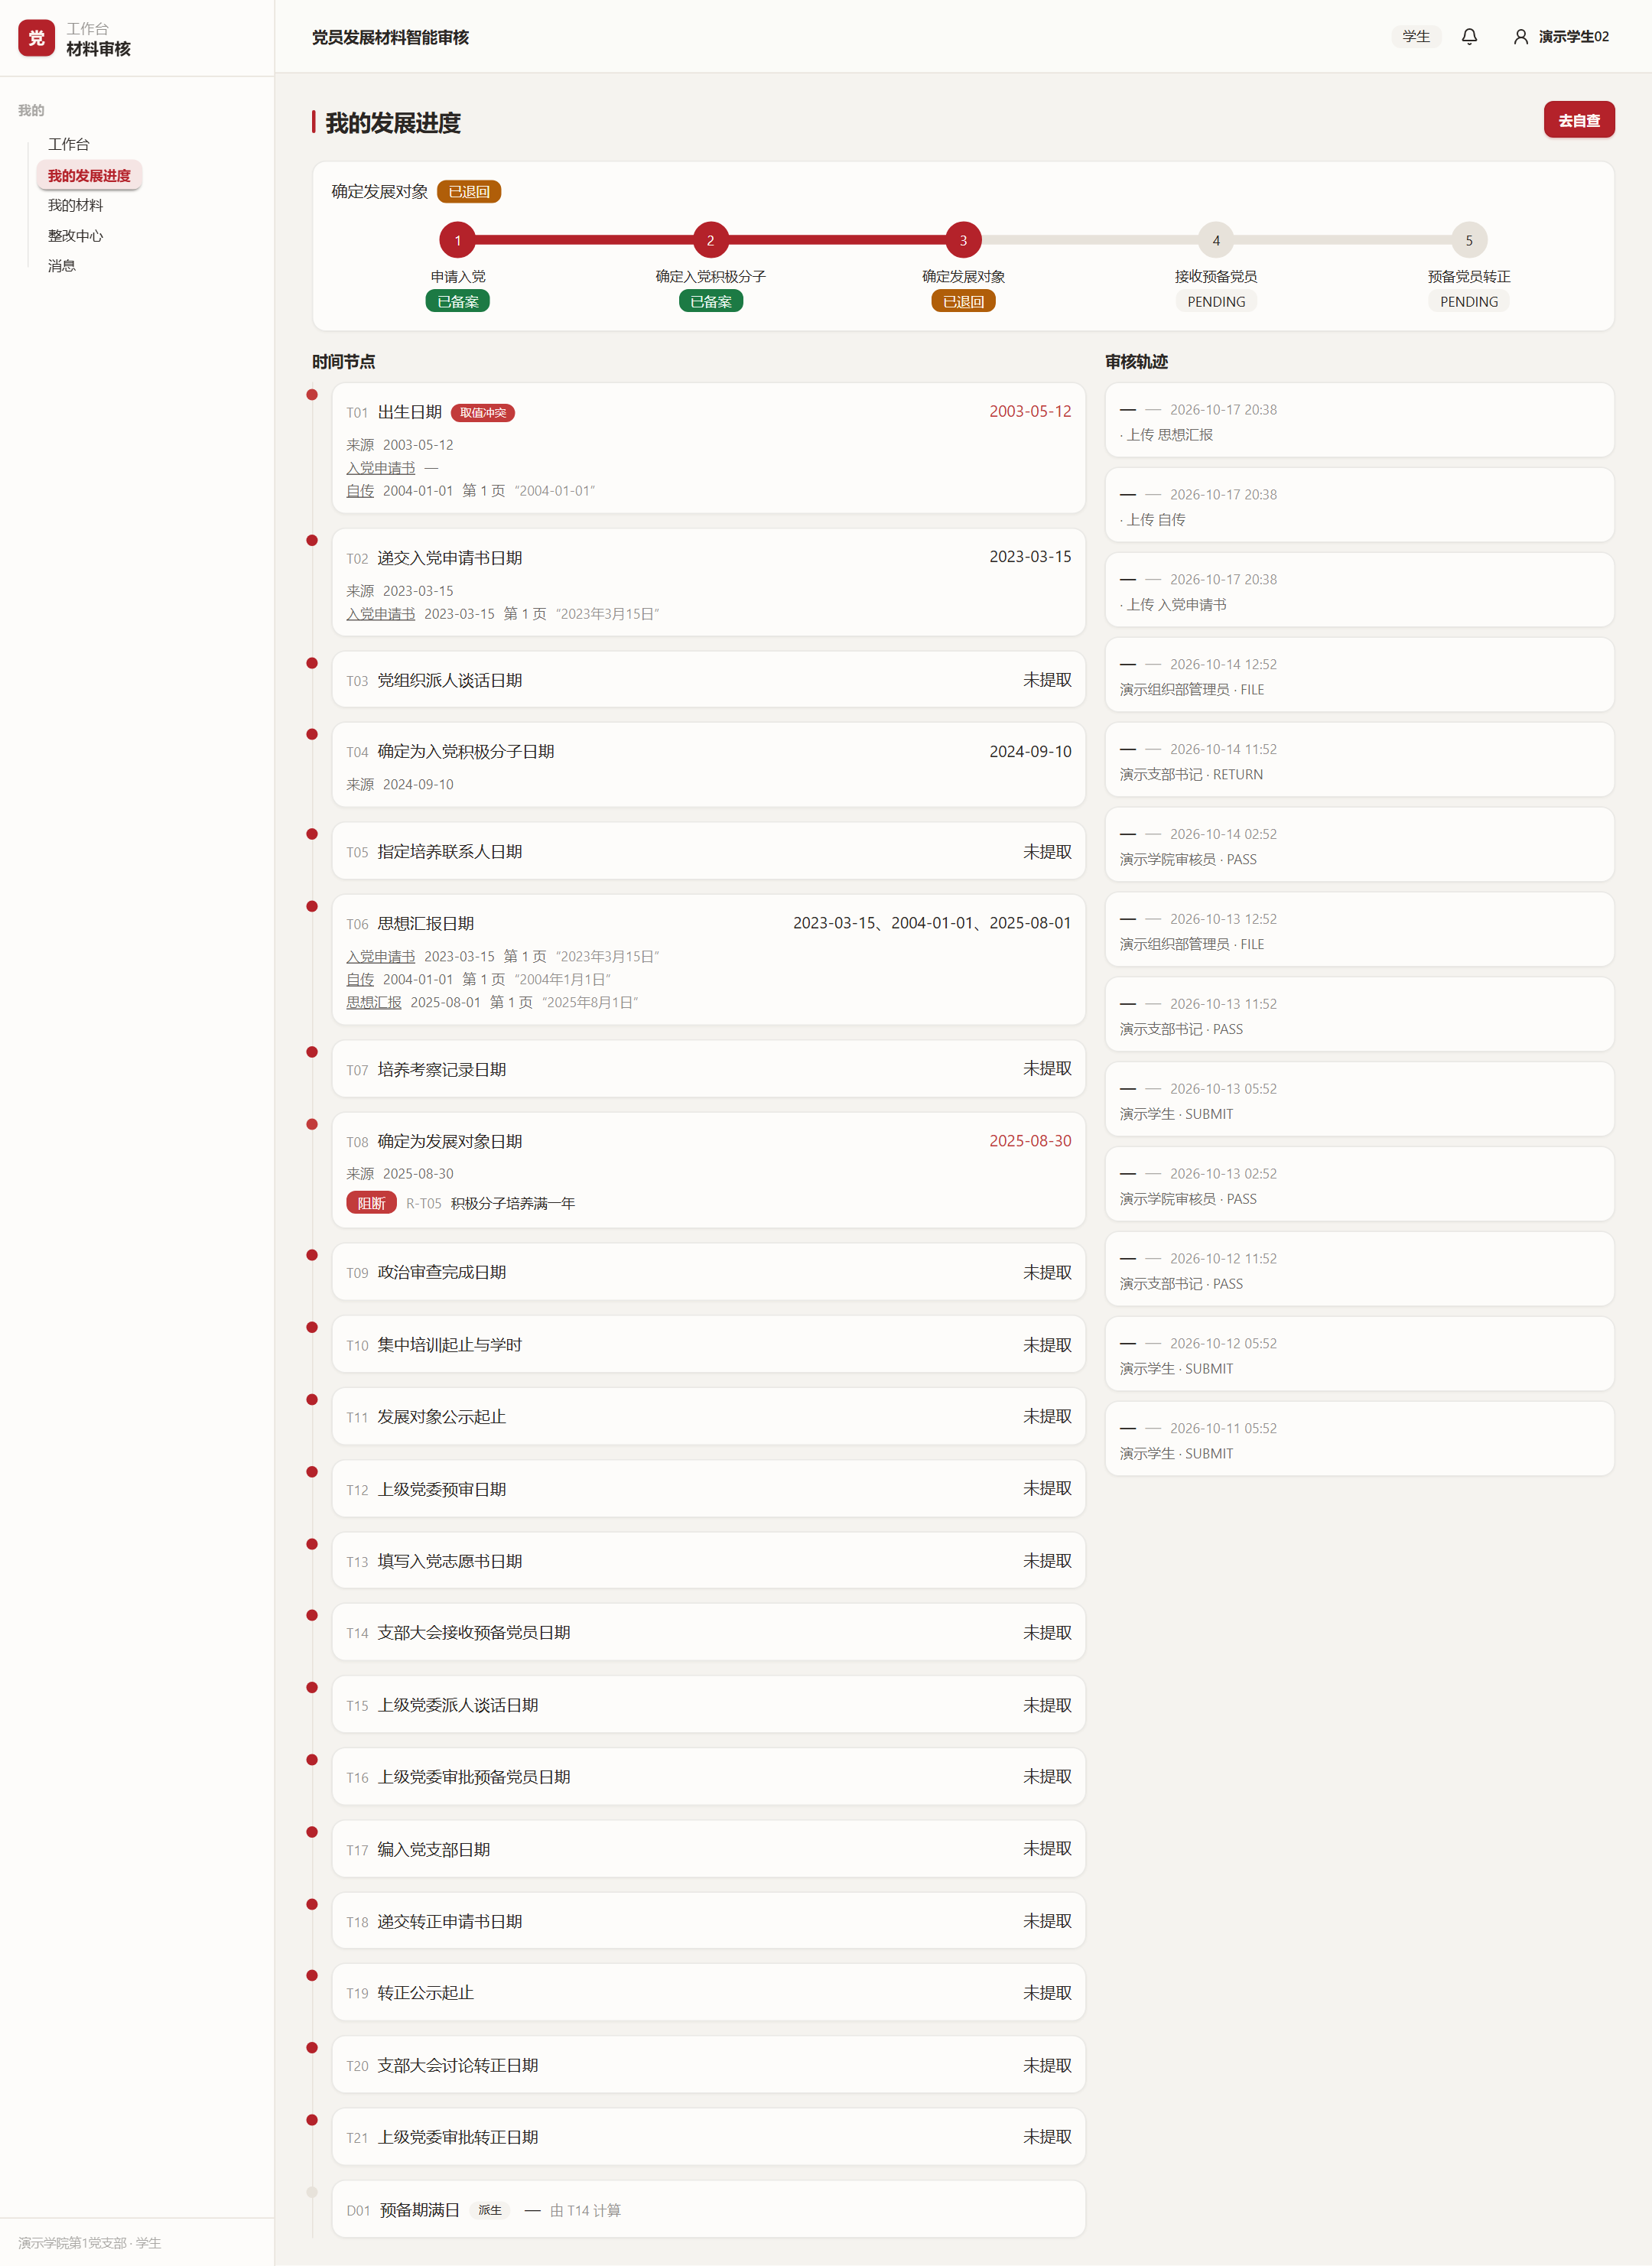
\includegraphics[width=\textwidth]{../figures/shot_student_progress.png}
    \caption{学生端阶段进度时间轴}
    \label{fig:ui-progress}
  \end{minipage}\hfill
  \begin{minipage}{0.48\textwidth}
    \centering
    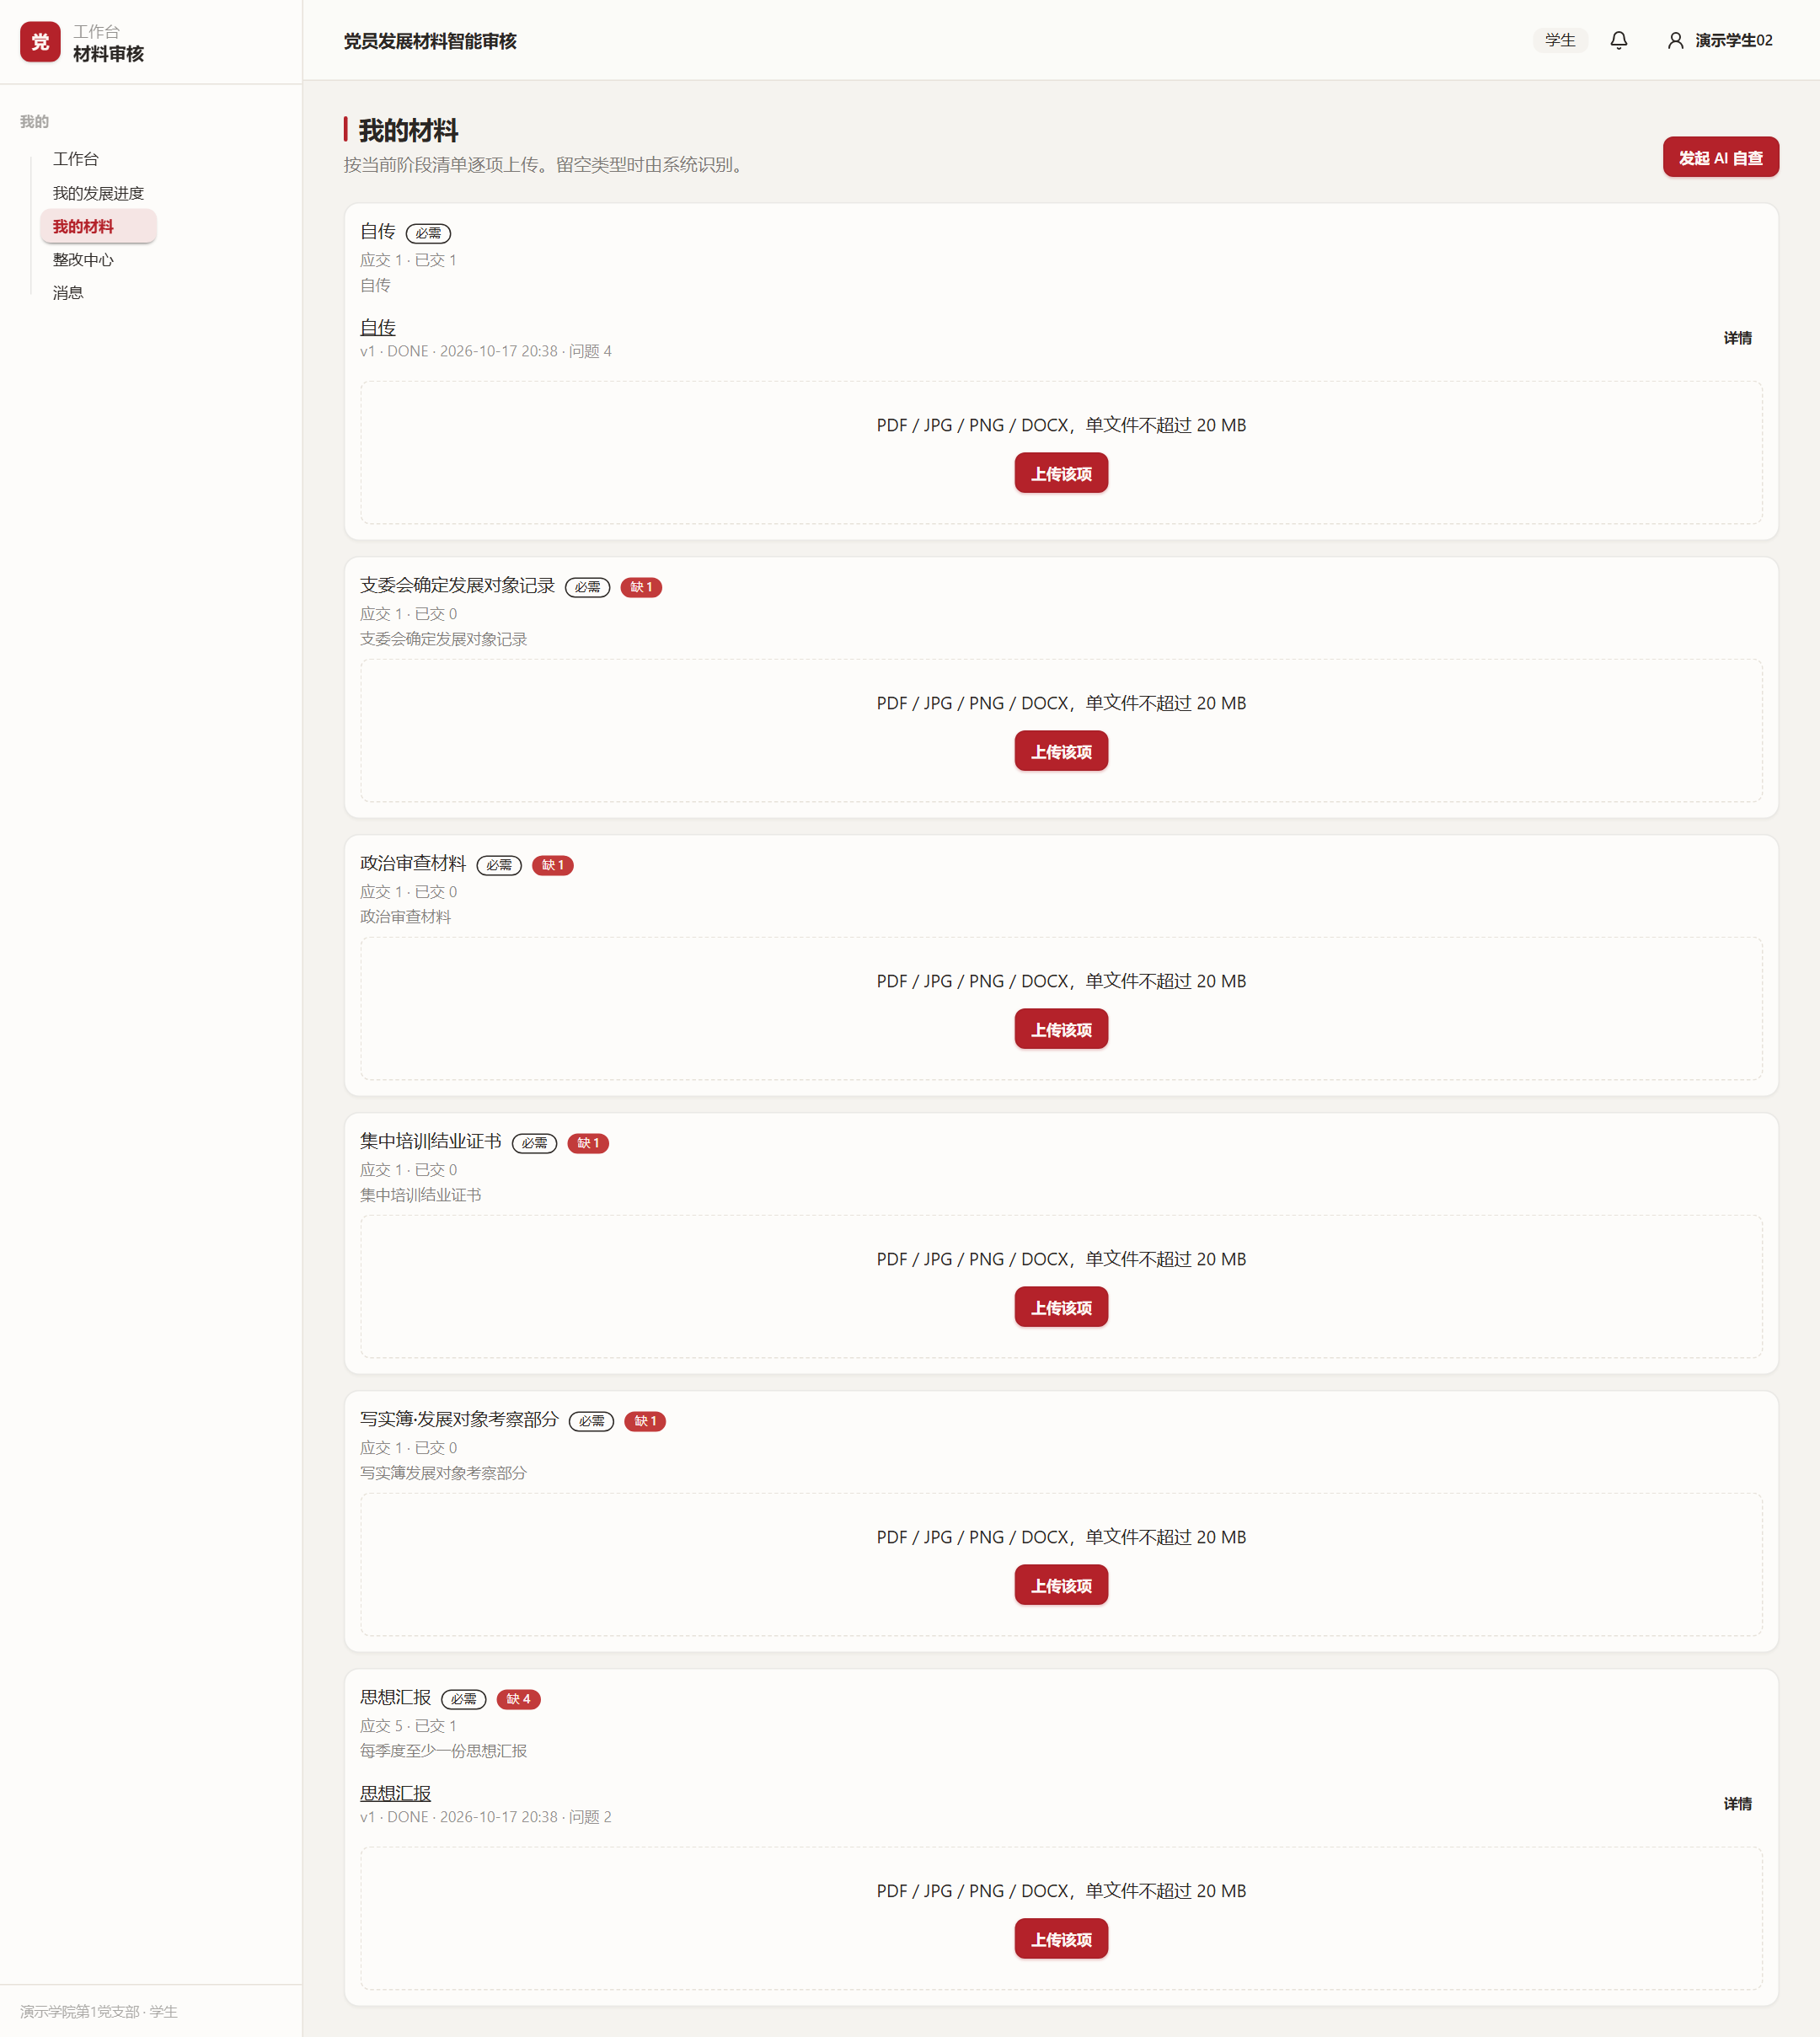
\includegraphics[width=\textwidth]{../figures/shot_student_materials.png}
    \caption{学生端我的材料}
    \label{fig:ui-materials}
  \end{minipage}
\end{figure}

图~\ref{fig:ui-selfcheck} 是学生发起自查后返回的报告，问题按完整性、时间、形式、内容分类并按阻断、警告、提示三级排序，每条问题附带规则依据、原文定位与修改建议；图~\ref{fig:ui-rectification} 是整改中心，学生需逐条回复整改情况，未回复的问题会阻止重新提交，提交后系统自动复核问题是否消除。

\begin{figure}[H]
  \centering
  \begin{minipage}{0.48\textwidth}
    \centering
    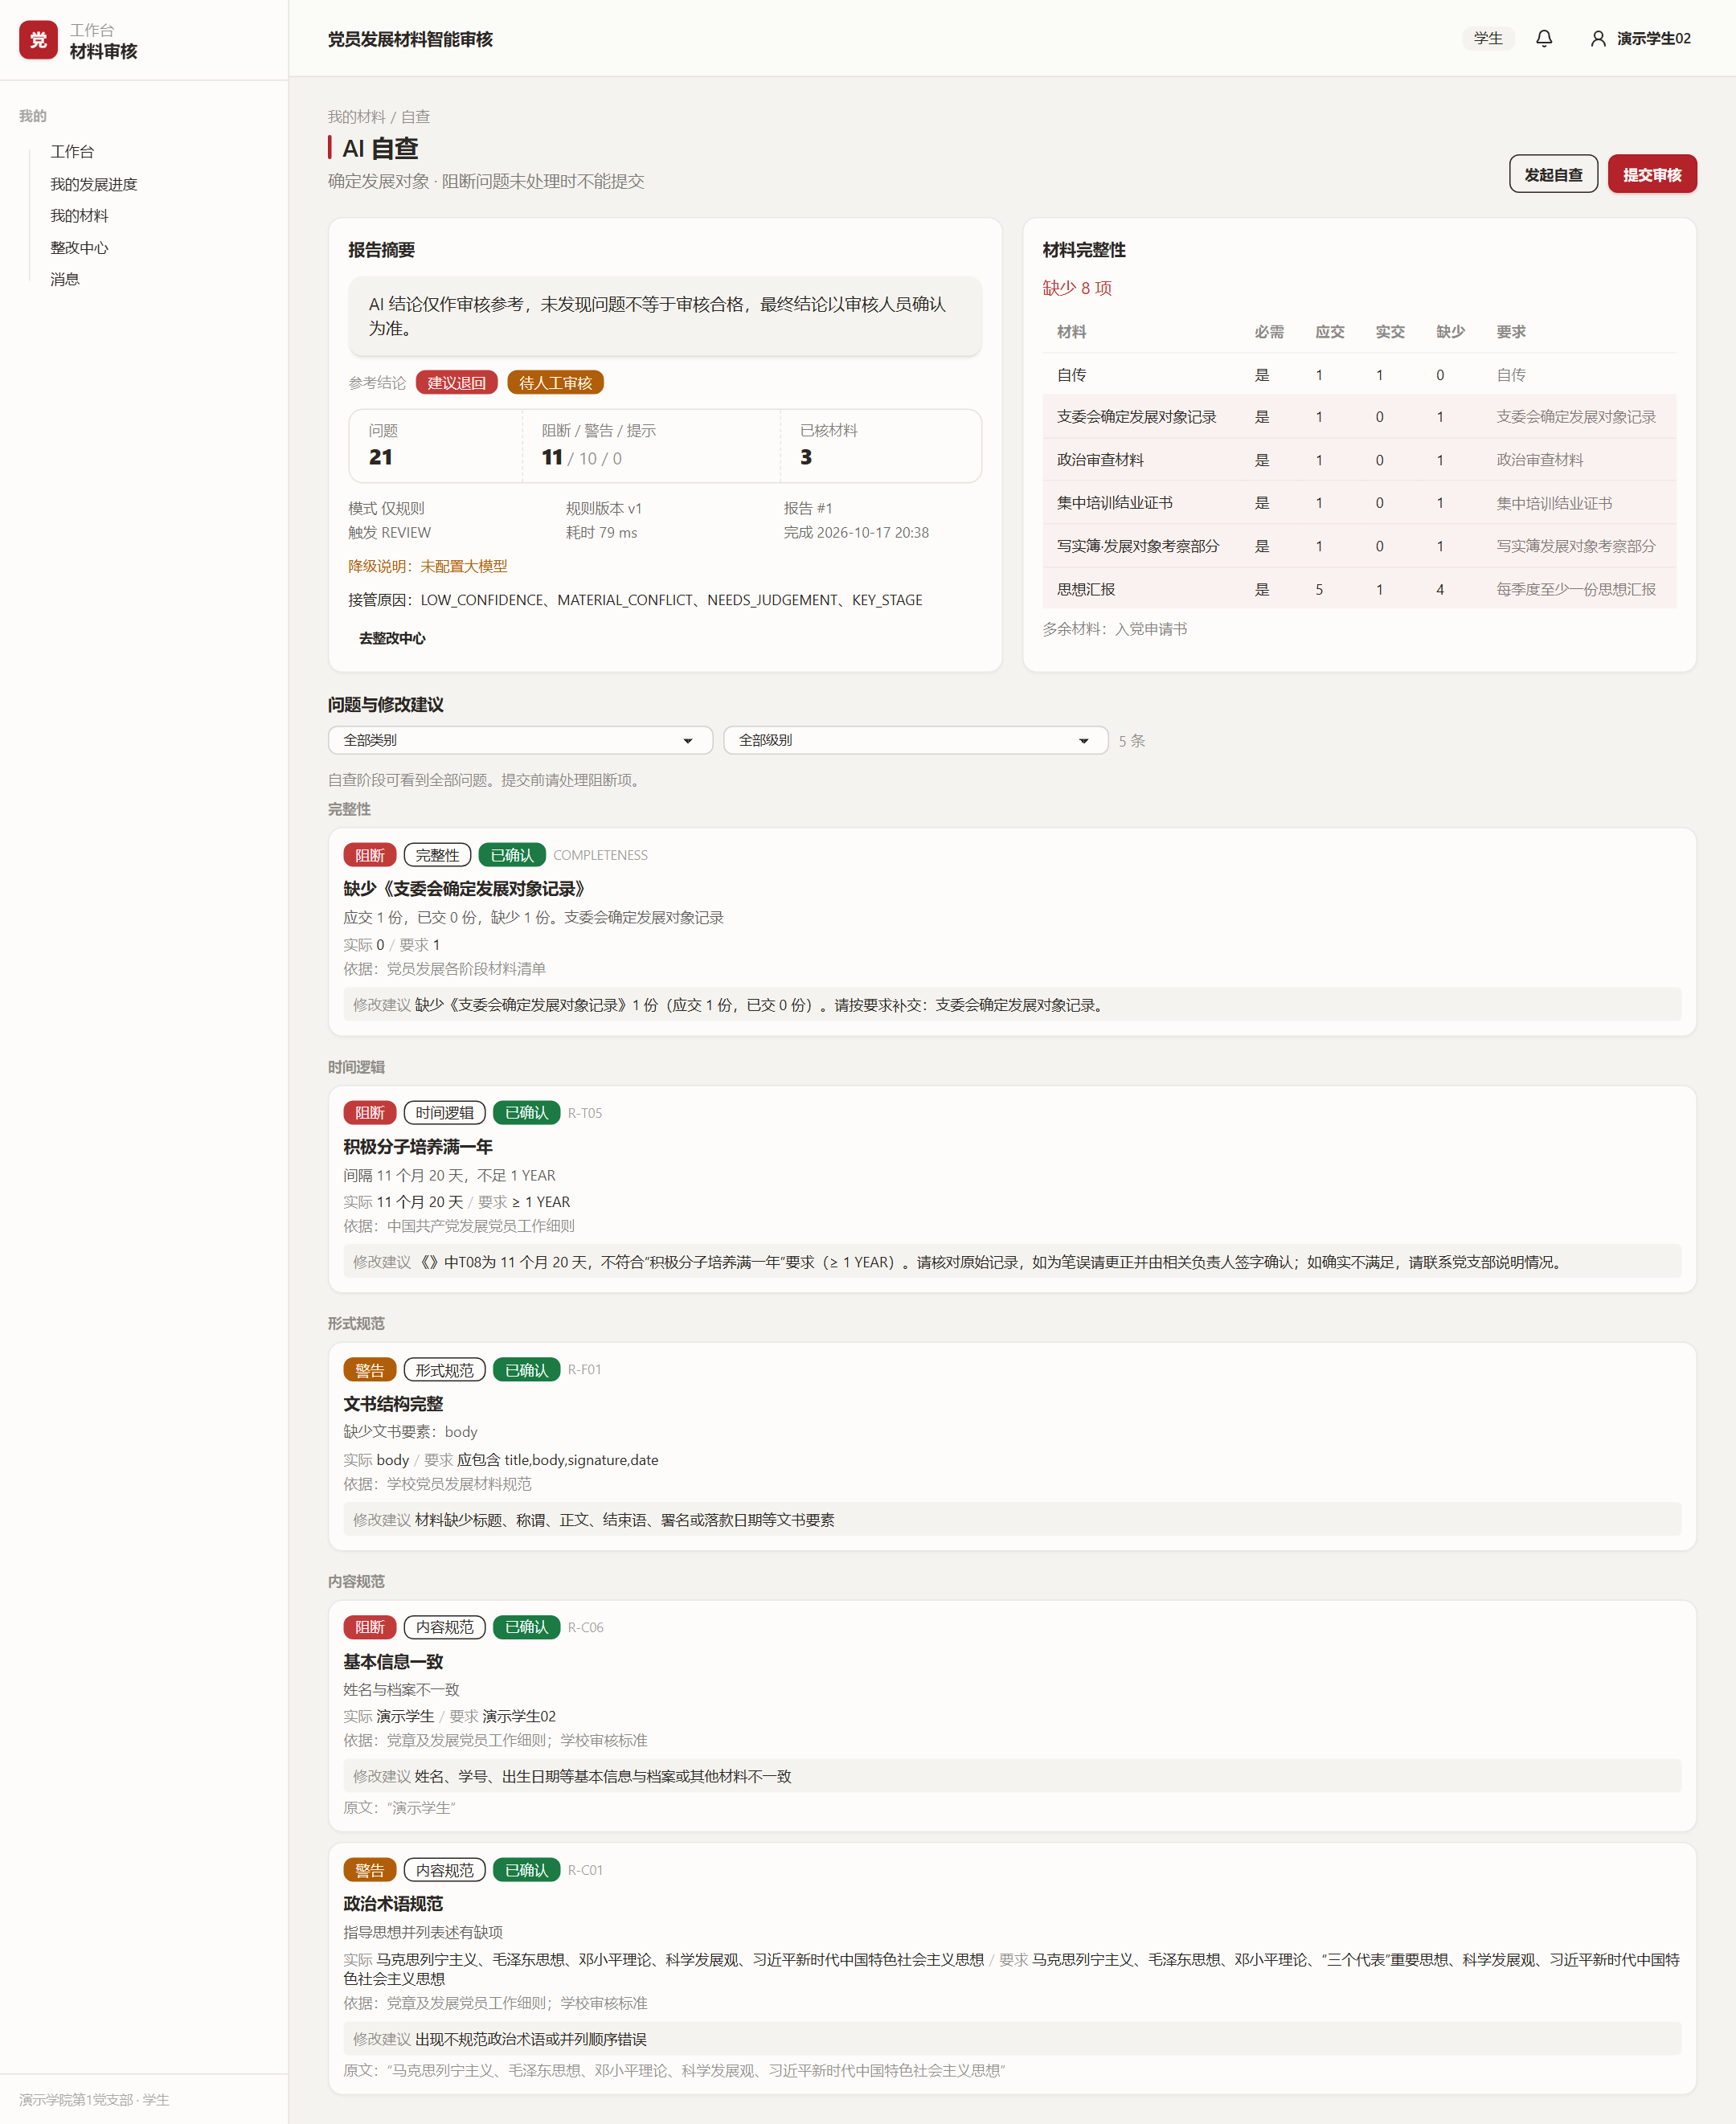
\includegraphics[width=\textwidth]{../figures/shot_student_selfcheck.png}
    \caption{AI 自查报告}
    \label{fig:ui-selfcheck}
  \end{minipage}\hfill
  \begin{minipage}{0.48\textwidth}
    \centering
    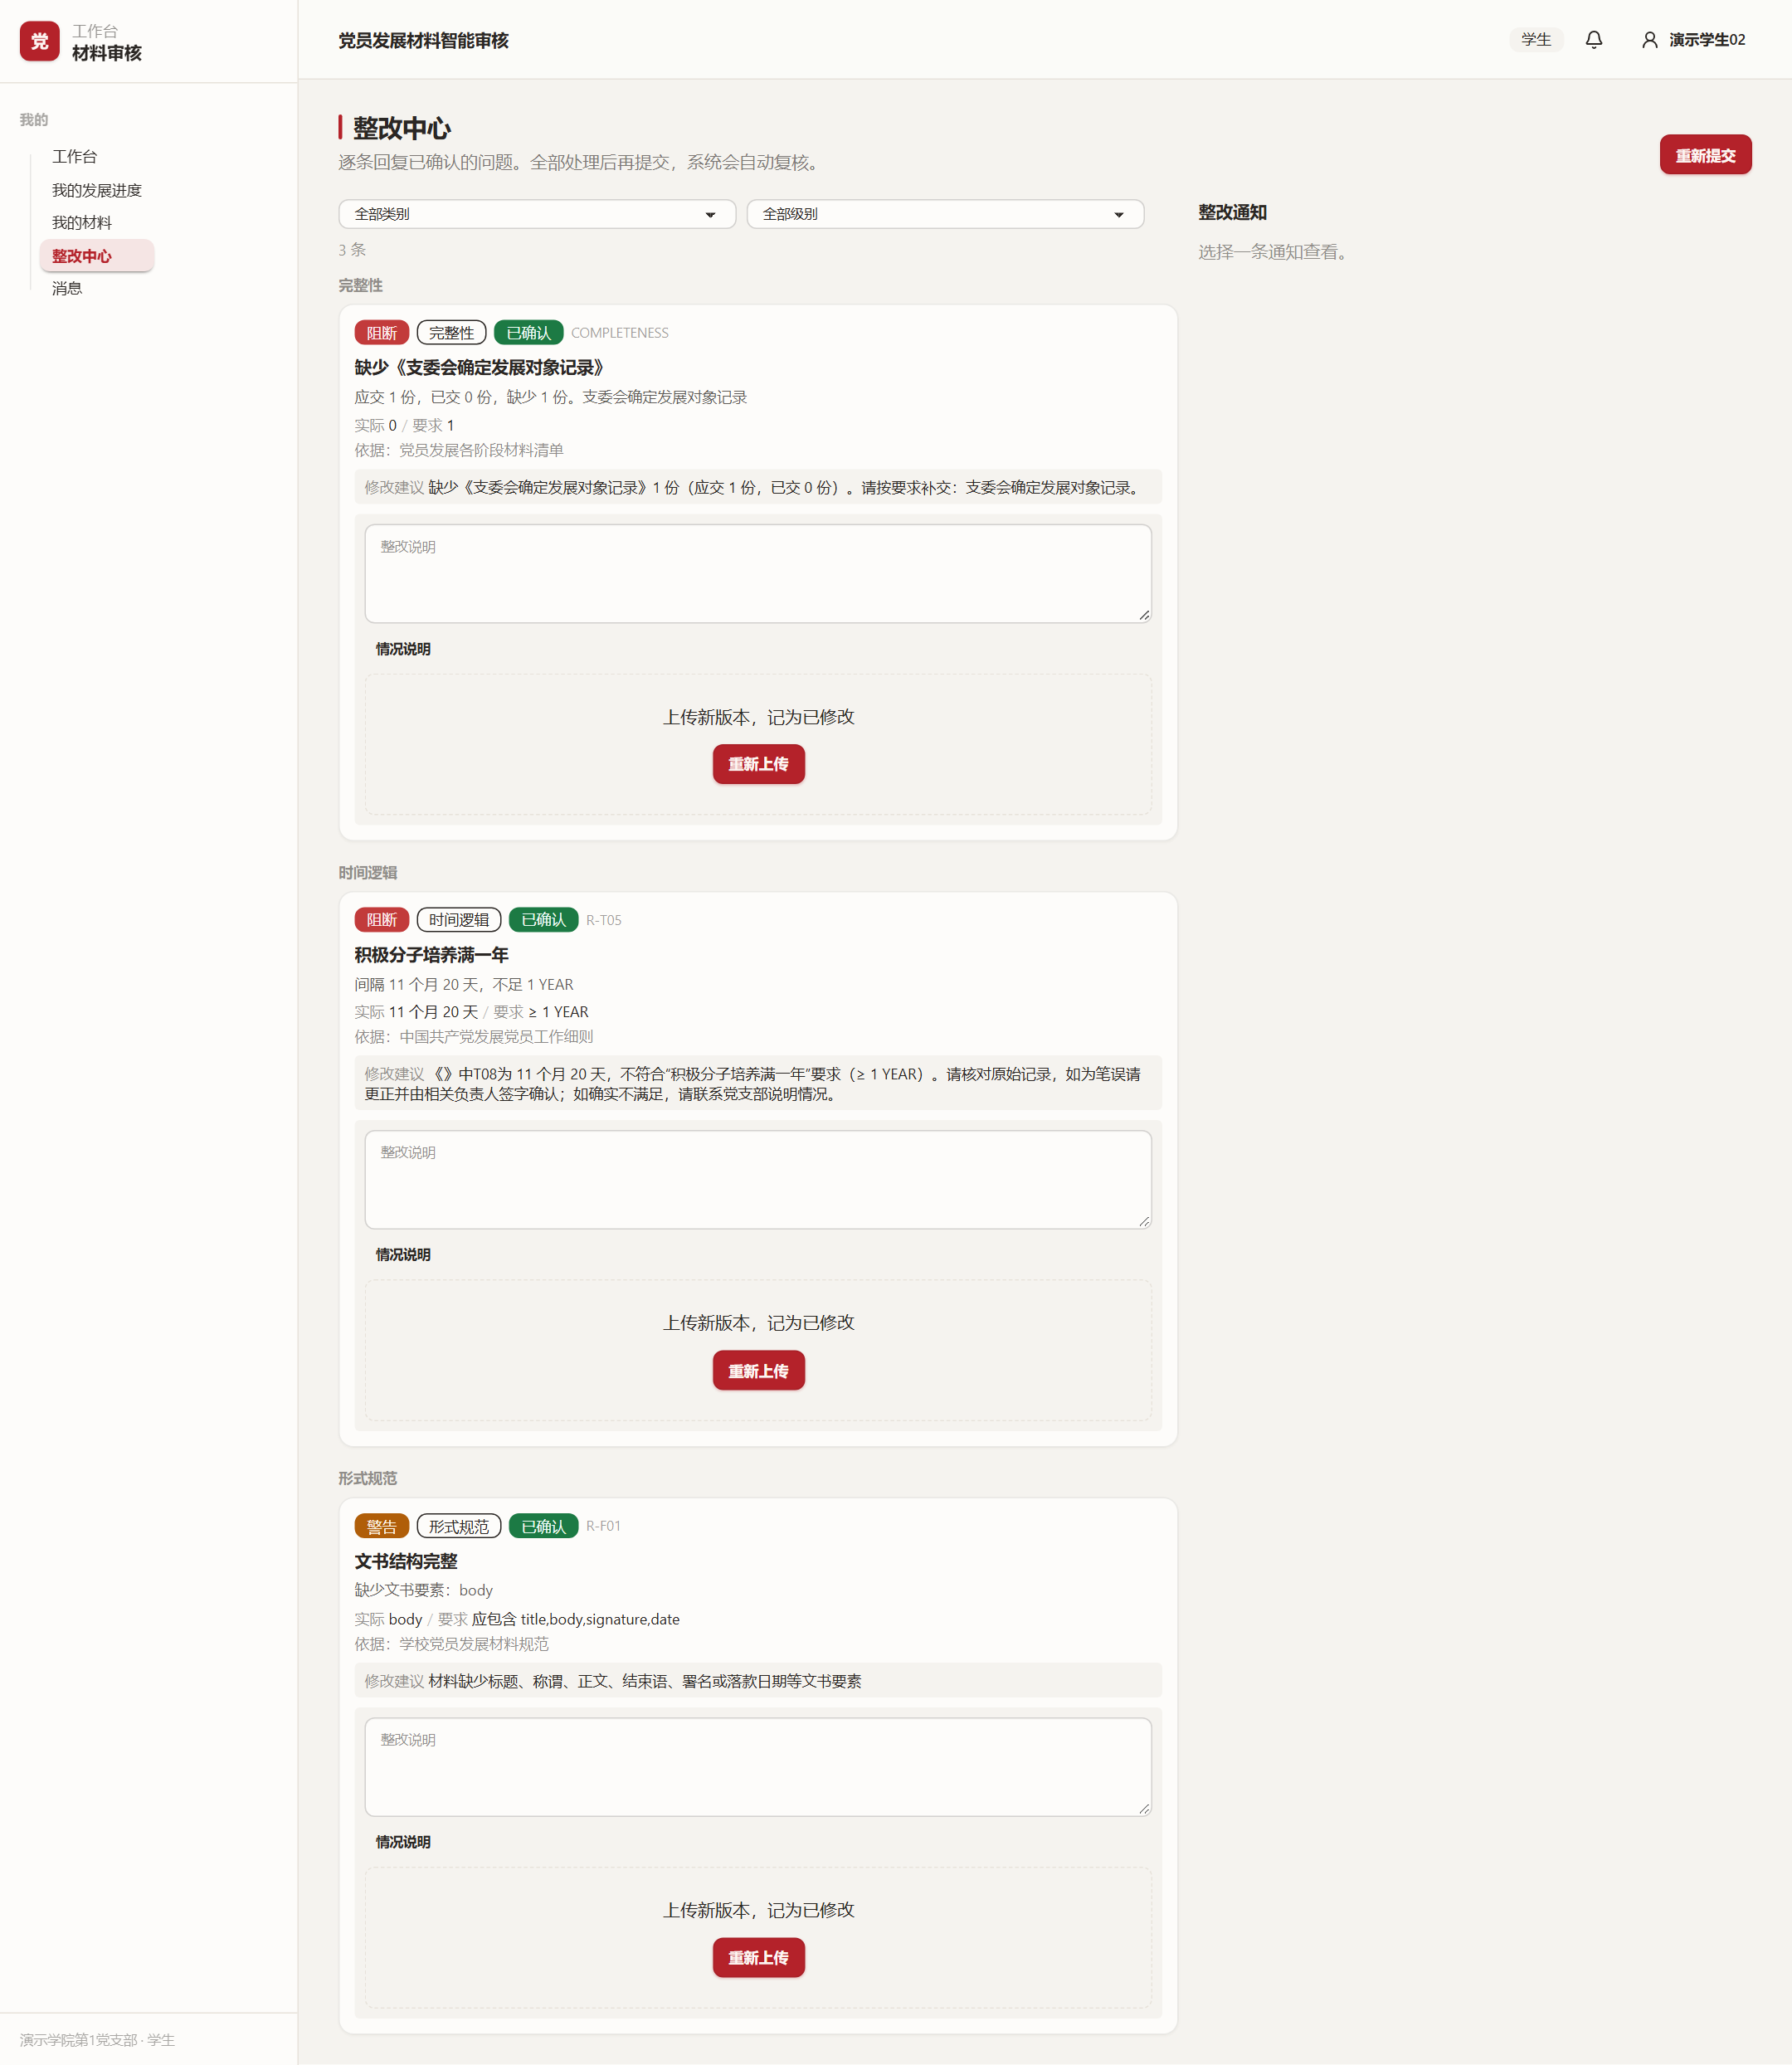
\includegraphics[width=\textwidth]{../figures/shot_student_rectification.png}
    \caption{学生整改中心}
    \label{fig:ui-rectification}
  \end{minipage}
\end{figure}

审核端的待办列表如图~\ref{fig:ui-tasks} 所示，可按阶段、批次与问题级别筛选；图~\ref{fig:ui-workspace} 是审核工作区，左侧逐页预览材料原文，右侧列出对应的问题清单与审核决定，选中一条问题后预览区自动定位到相关页面，审核员可确认问题、驳回误报或手动补充问题。

\begin{figure}[H]
  \centering
  \begin{minipage}{0.48\textwidth}
    \centering
    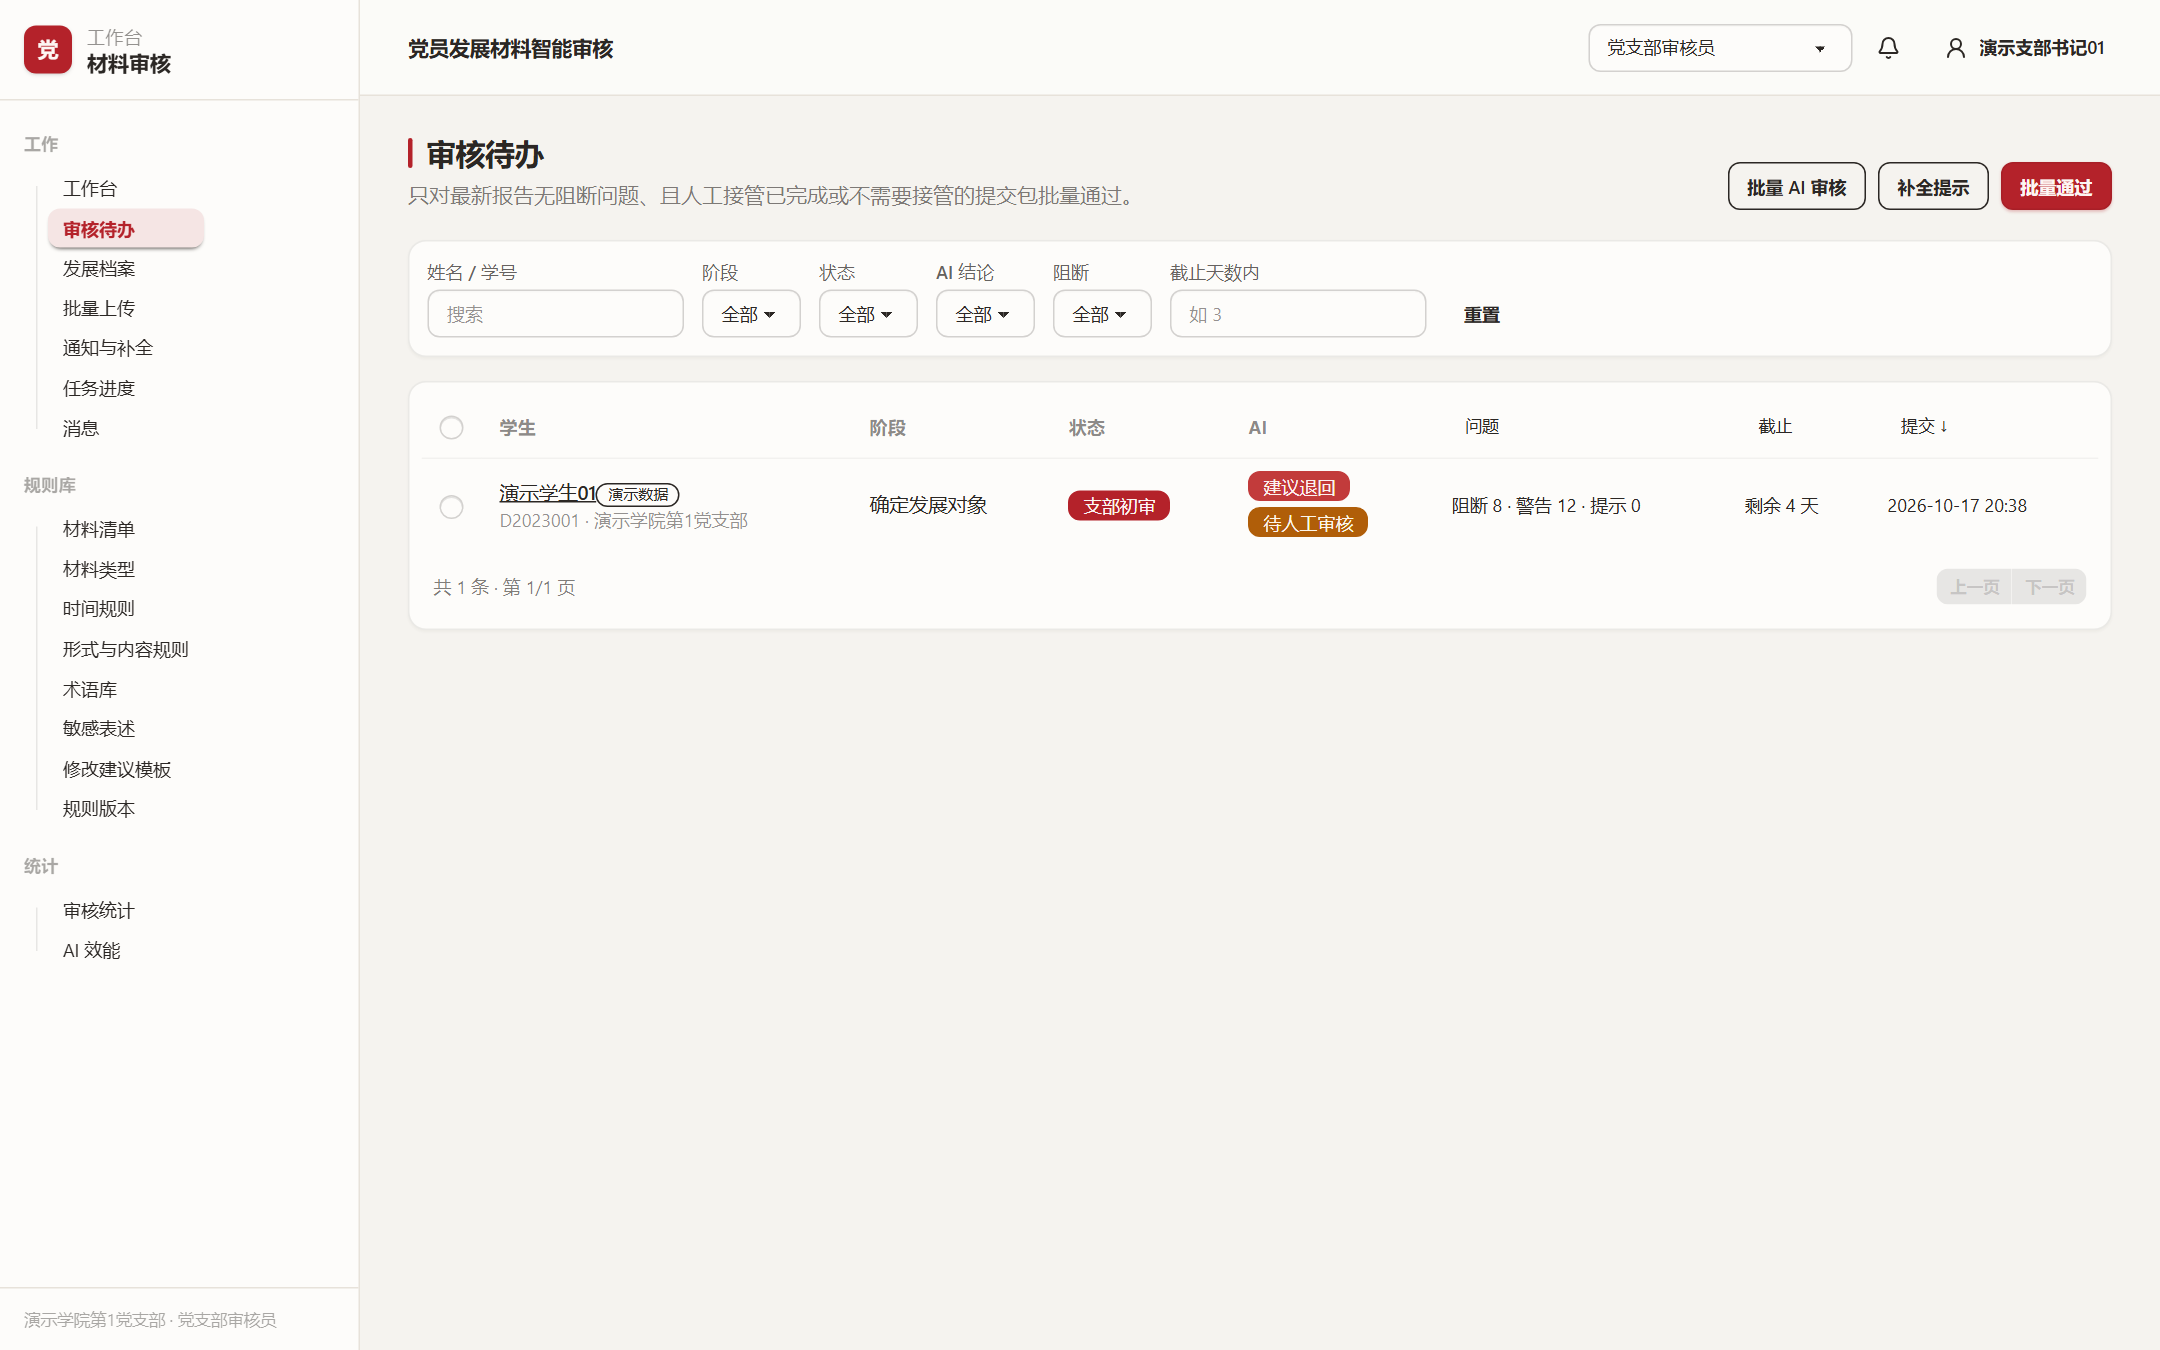
\includegraphics[width=\textwidth]{../figures/shot_review_tasks.png}
    \caption{审核待办}
    \label{fig:ui-tasks}
  \end{minipage}\hfill
  \begin{minipage}{0.48\textwidth}
    \centering
    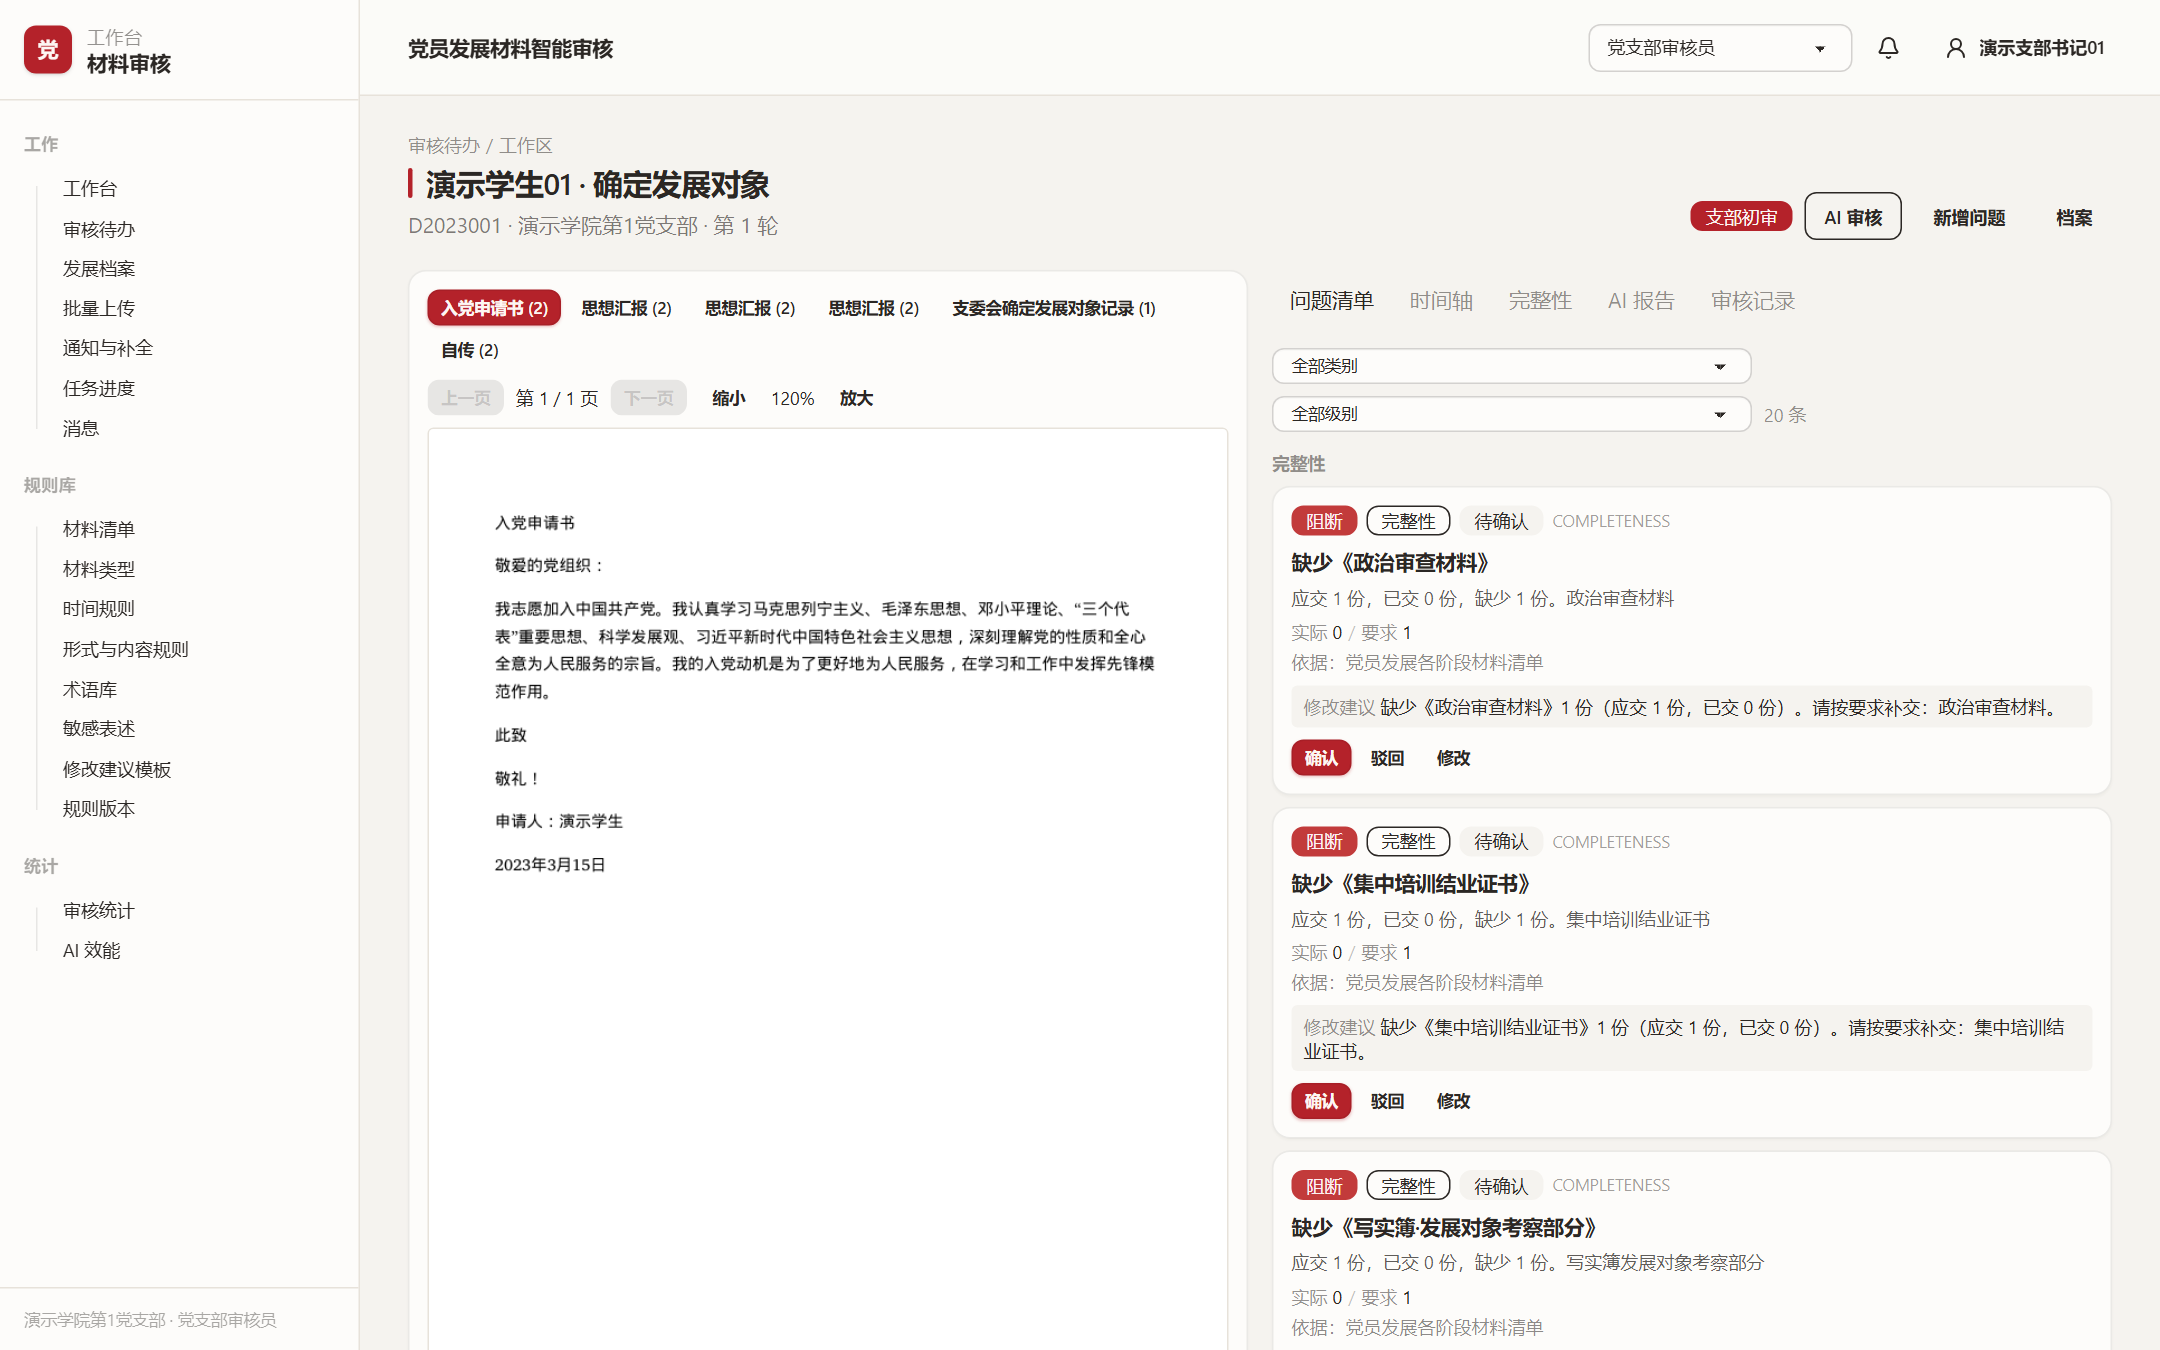
\includegraphics[width=\textwidth]{../figures/shot_review_workspace.png}
    \caption{审核工作区（左预览右问题）}
    \label{fig:ui-workspace}
  \end{minipage}
\end{figure}

管理侧提供统计与规则维护两类页面。图~\ref{fig:ui-stats} 的审核统计看板按问题类别、级别、支部与阶段汇总分布并展示流转趋势；图~\ref{fig:ui-rules-time} 是时间规则配置页，业务人员可直接增改算子参数并启停规则，无需改动代码，每次修改都生成新的规则版本。

\begin{figure}[H]
  \centering
  \begin{minipage}{0.48\textwidth}
    \centering
    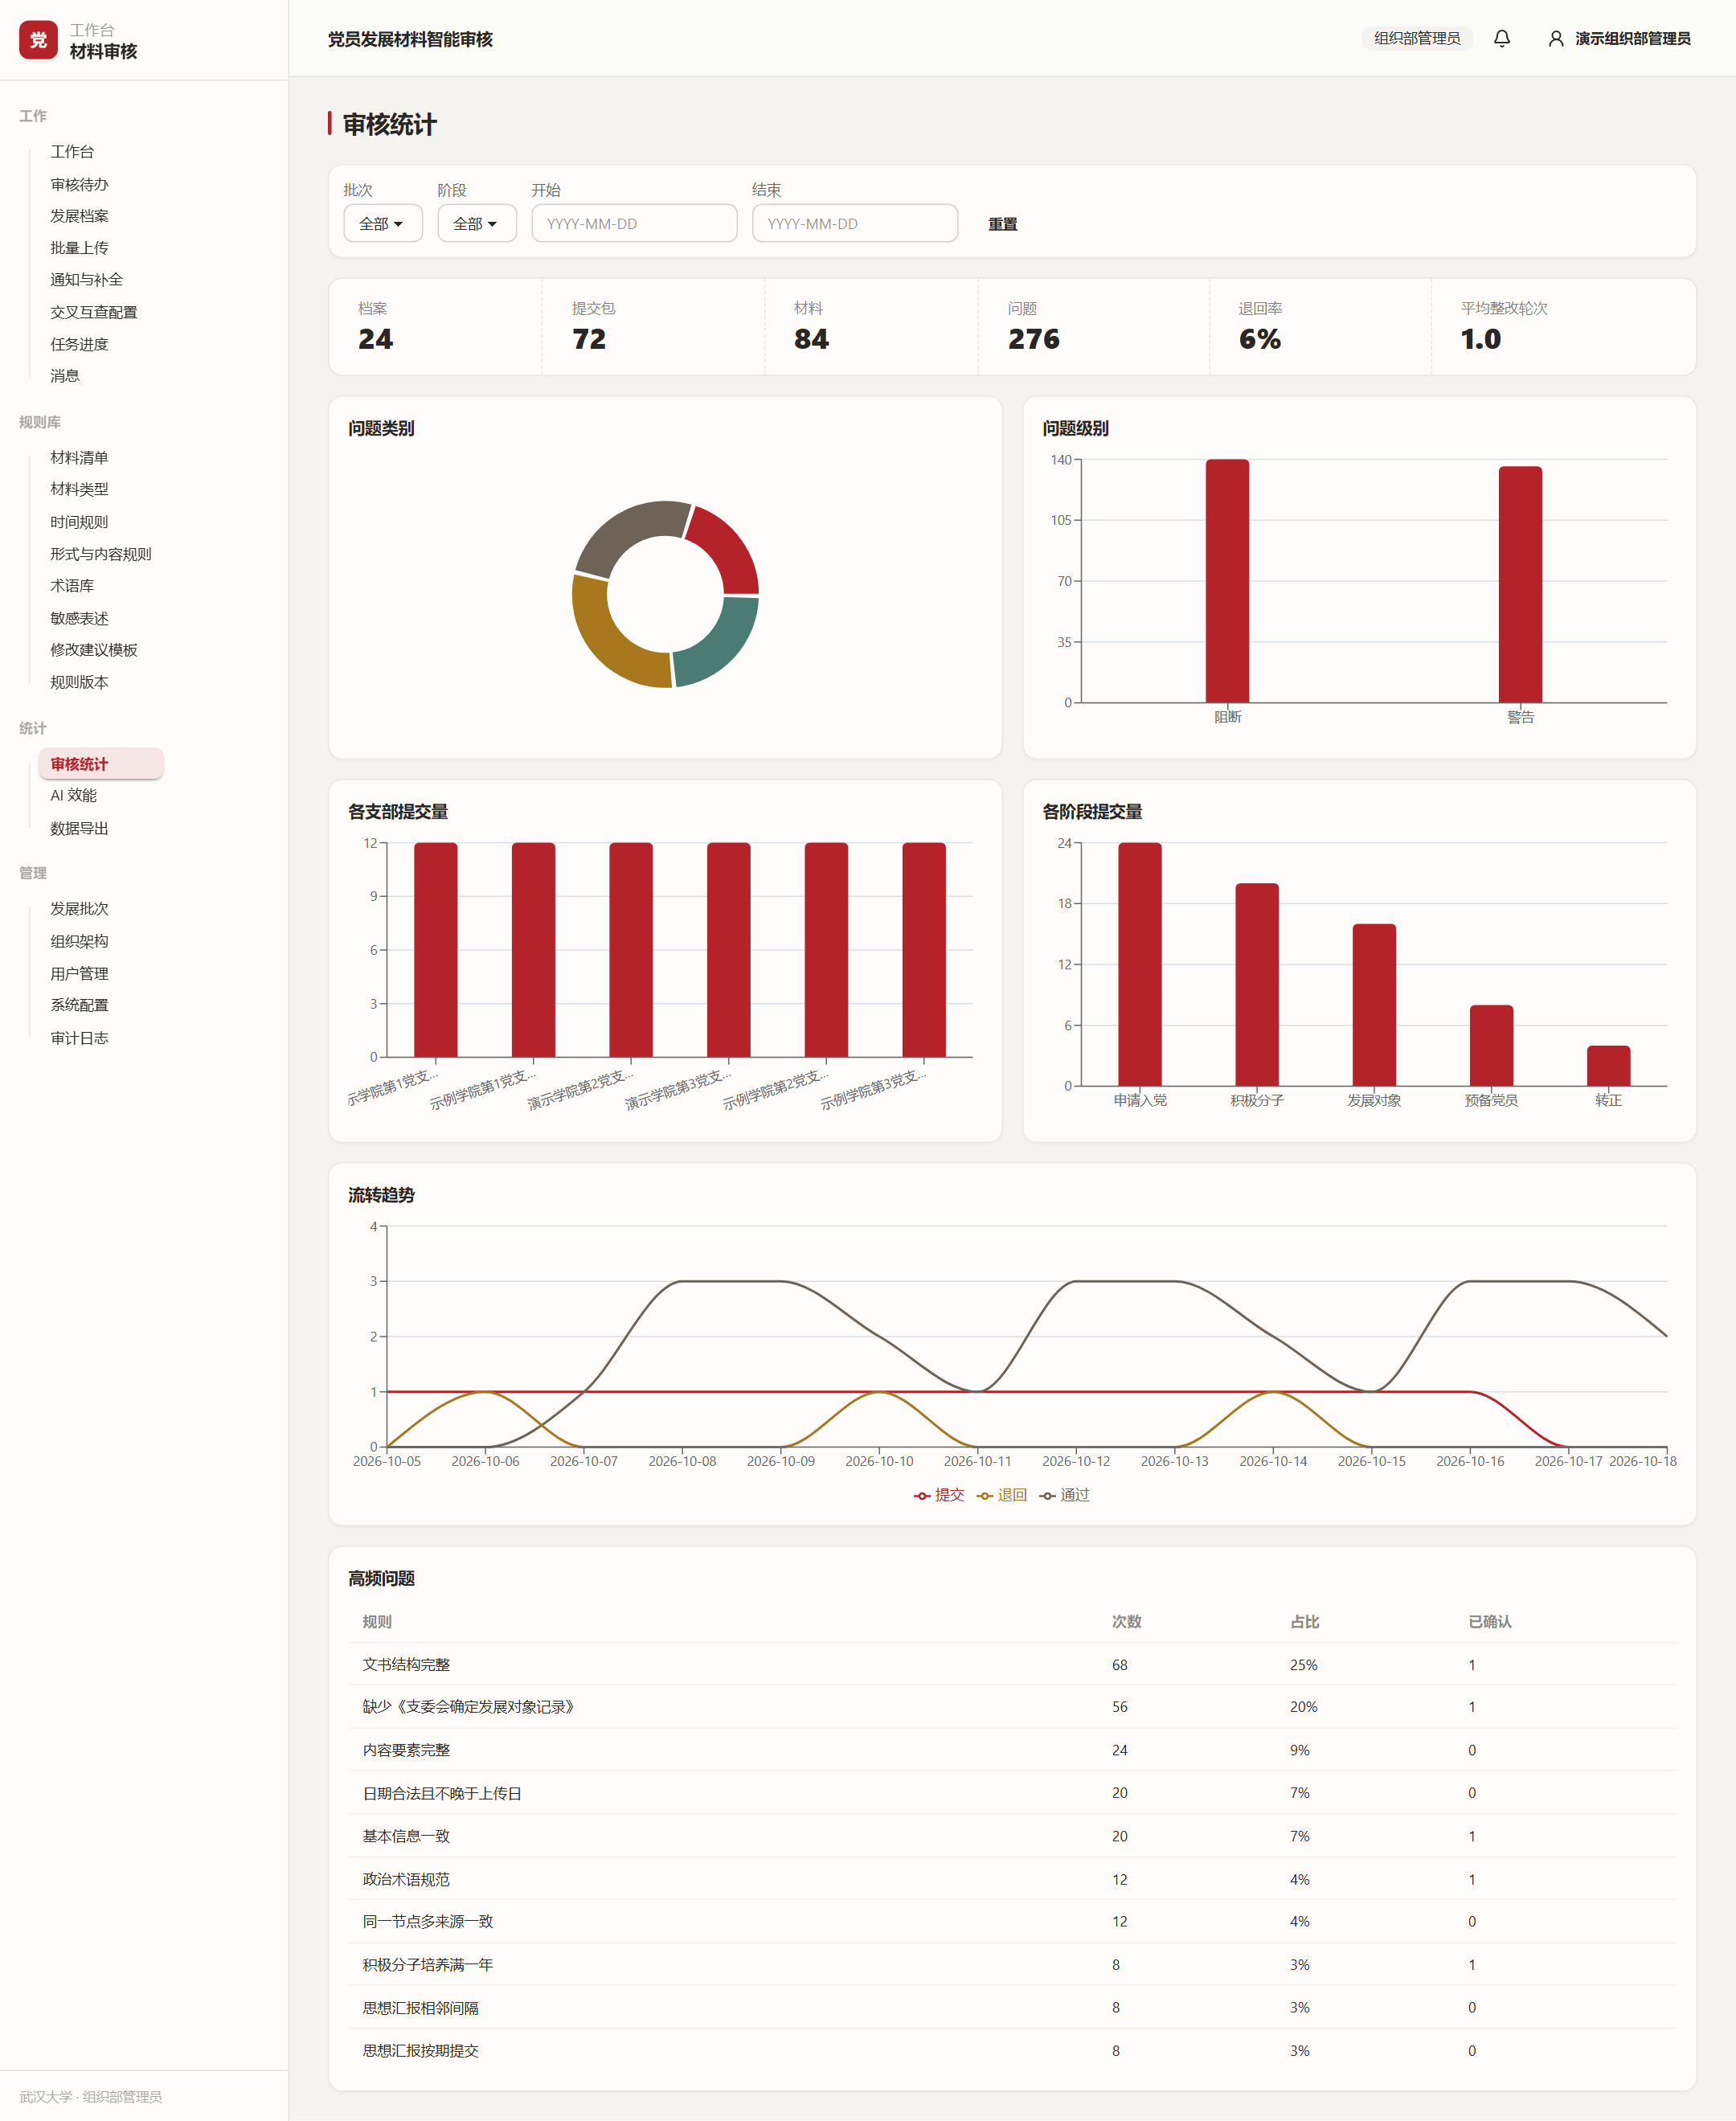
\includegraphics[width=\textwidth]{../figures/shot_stats_overview.png}
    \caption{审核统计看板}
    \label{fig:ui-stats}
  \end{minipage}\hfill
  \begin{minipage}{0.48\textwidth}
    \centering
    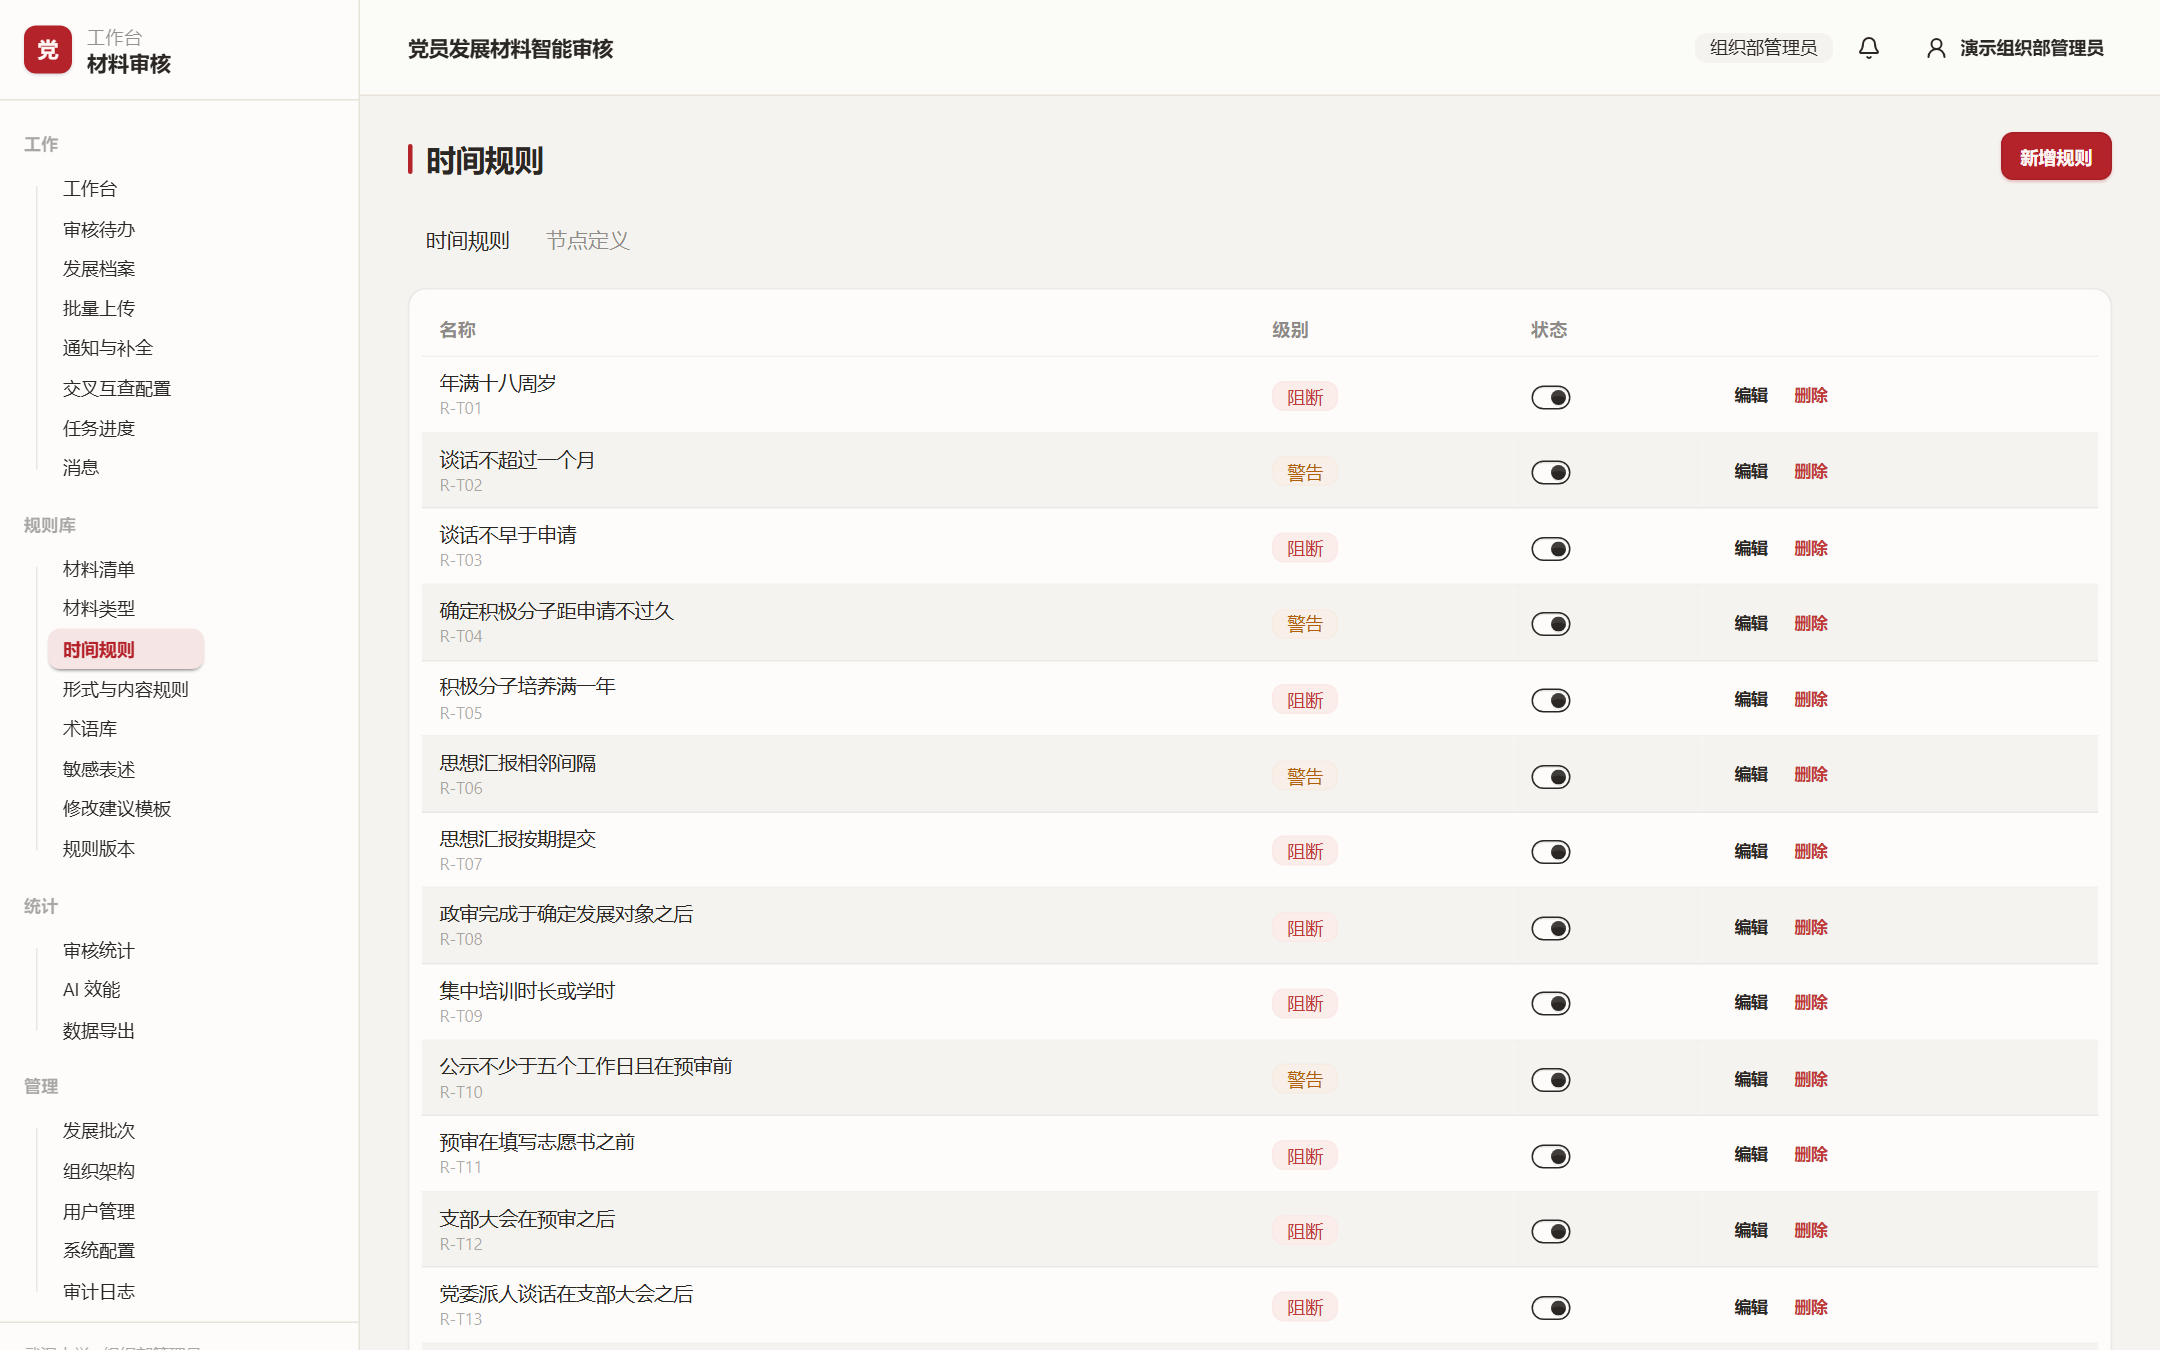
\includegraphics[width=\textwidth]{../figures/shot_rules_time.png}
    \caption{时间规则配置}
    \label{fig:ui-rules-time}
  \end{minipage}
\end{figure}

图~\ref{fig:ui-rules-terms} 是政治术语库，支持术语的增删改查与表格导入导出，内容校验时据此匹配不规范表述；图~\ref{fig:ui-audit} 是审计日志，登录、上传、审核、导出与规则变更均按时间顺序留痕，日志不提供删除入口，保证审核过程可追溯、可问责。

\begin{figure}[H]
  \centering
  \begin{minipage}{0.48\textwidth}
    \centering
    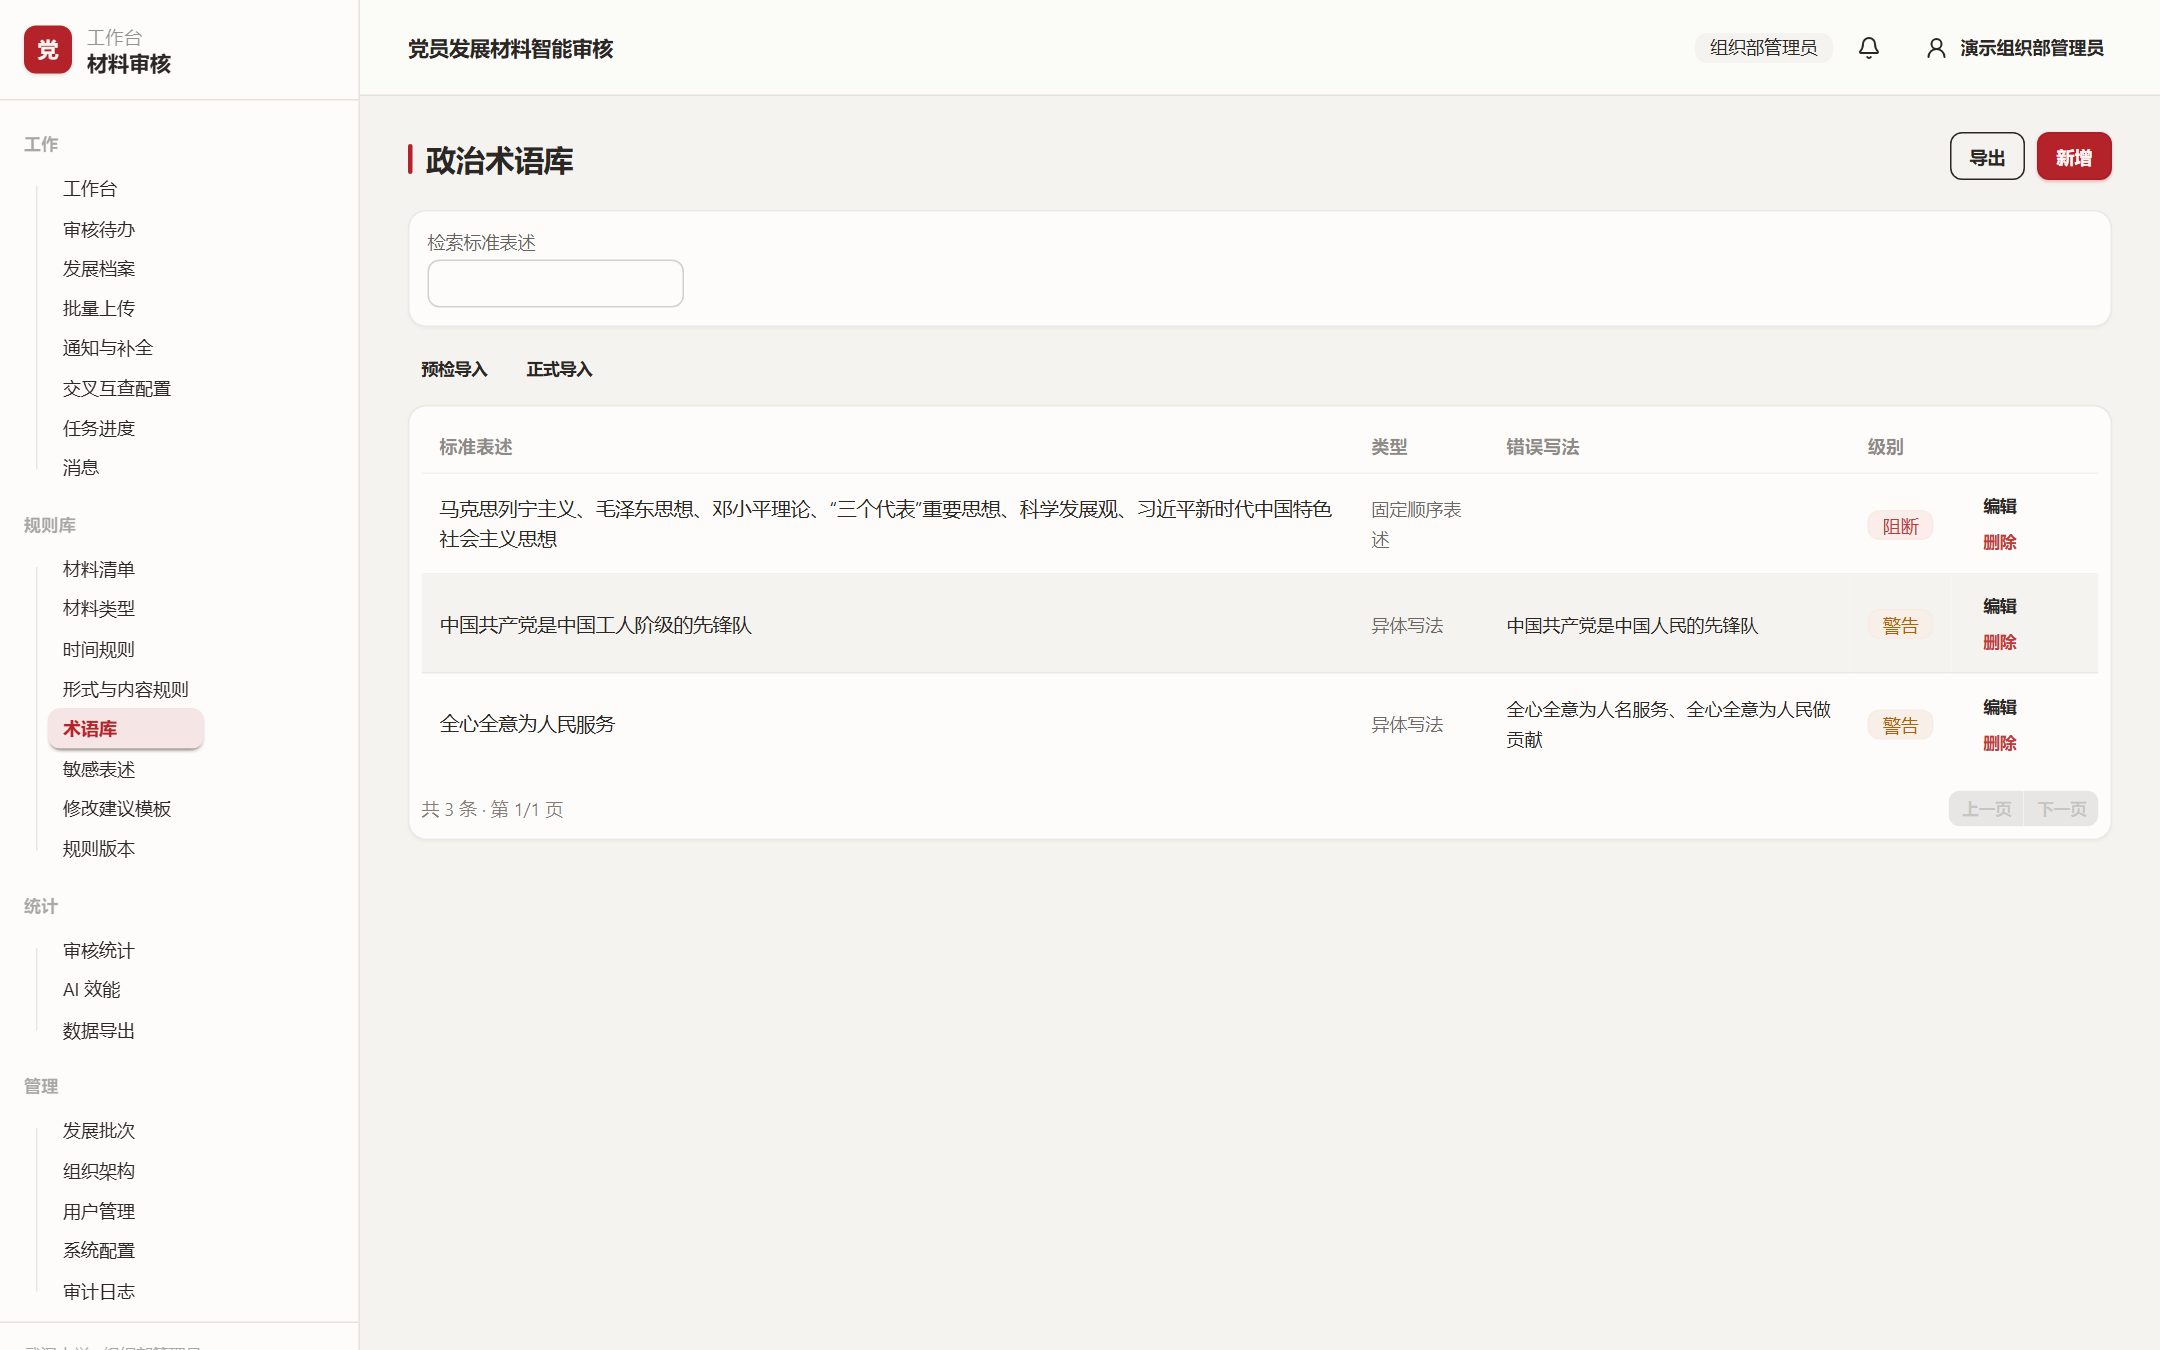
\includegraphics[width=\textwidth]{../figures/shot_rules_terms.png}
    \caption{政治术语库}
    \label{fig:ui-rules-terms}
  \end{minipage}\hfill
  \begin{minipage}{0.48\textwidth}
    \centering
    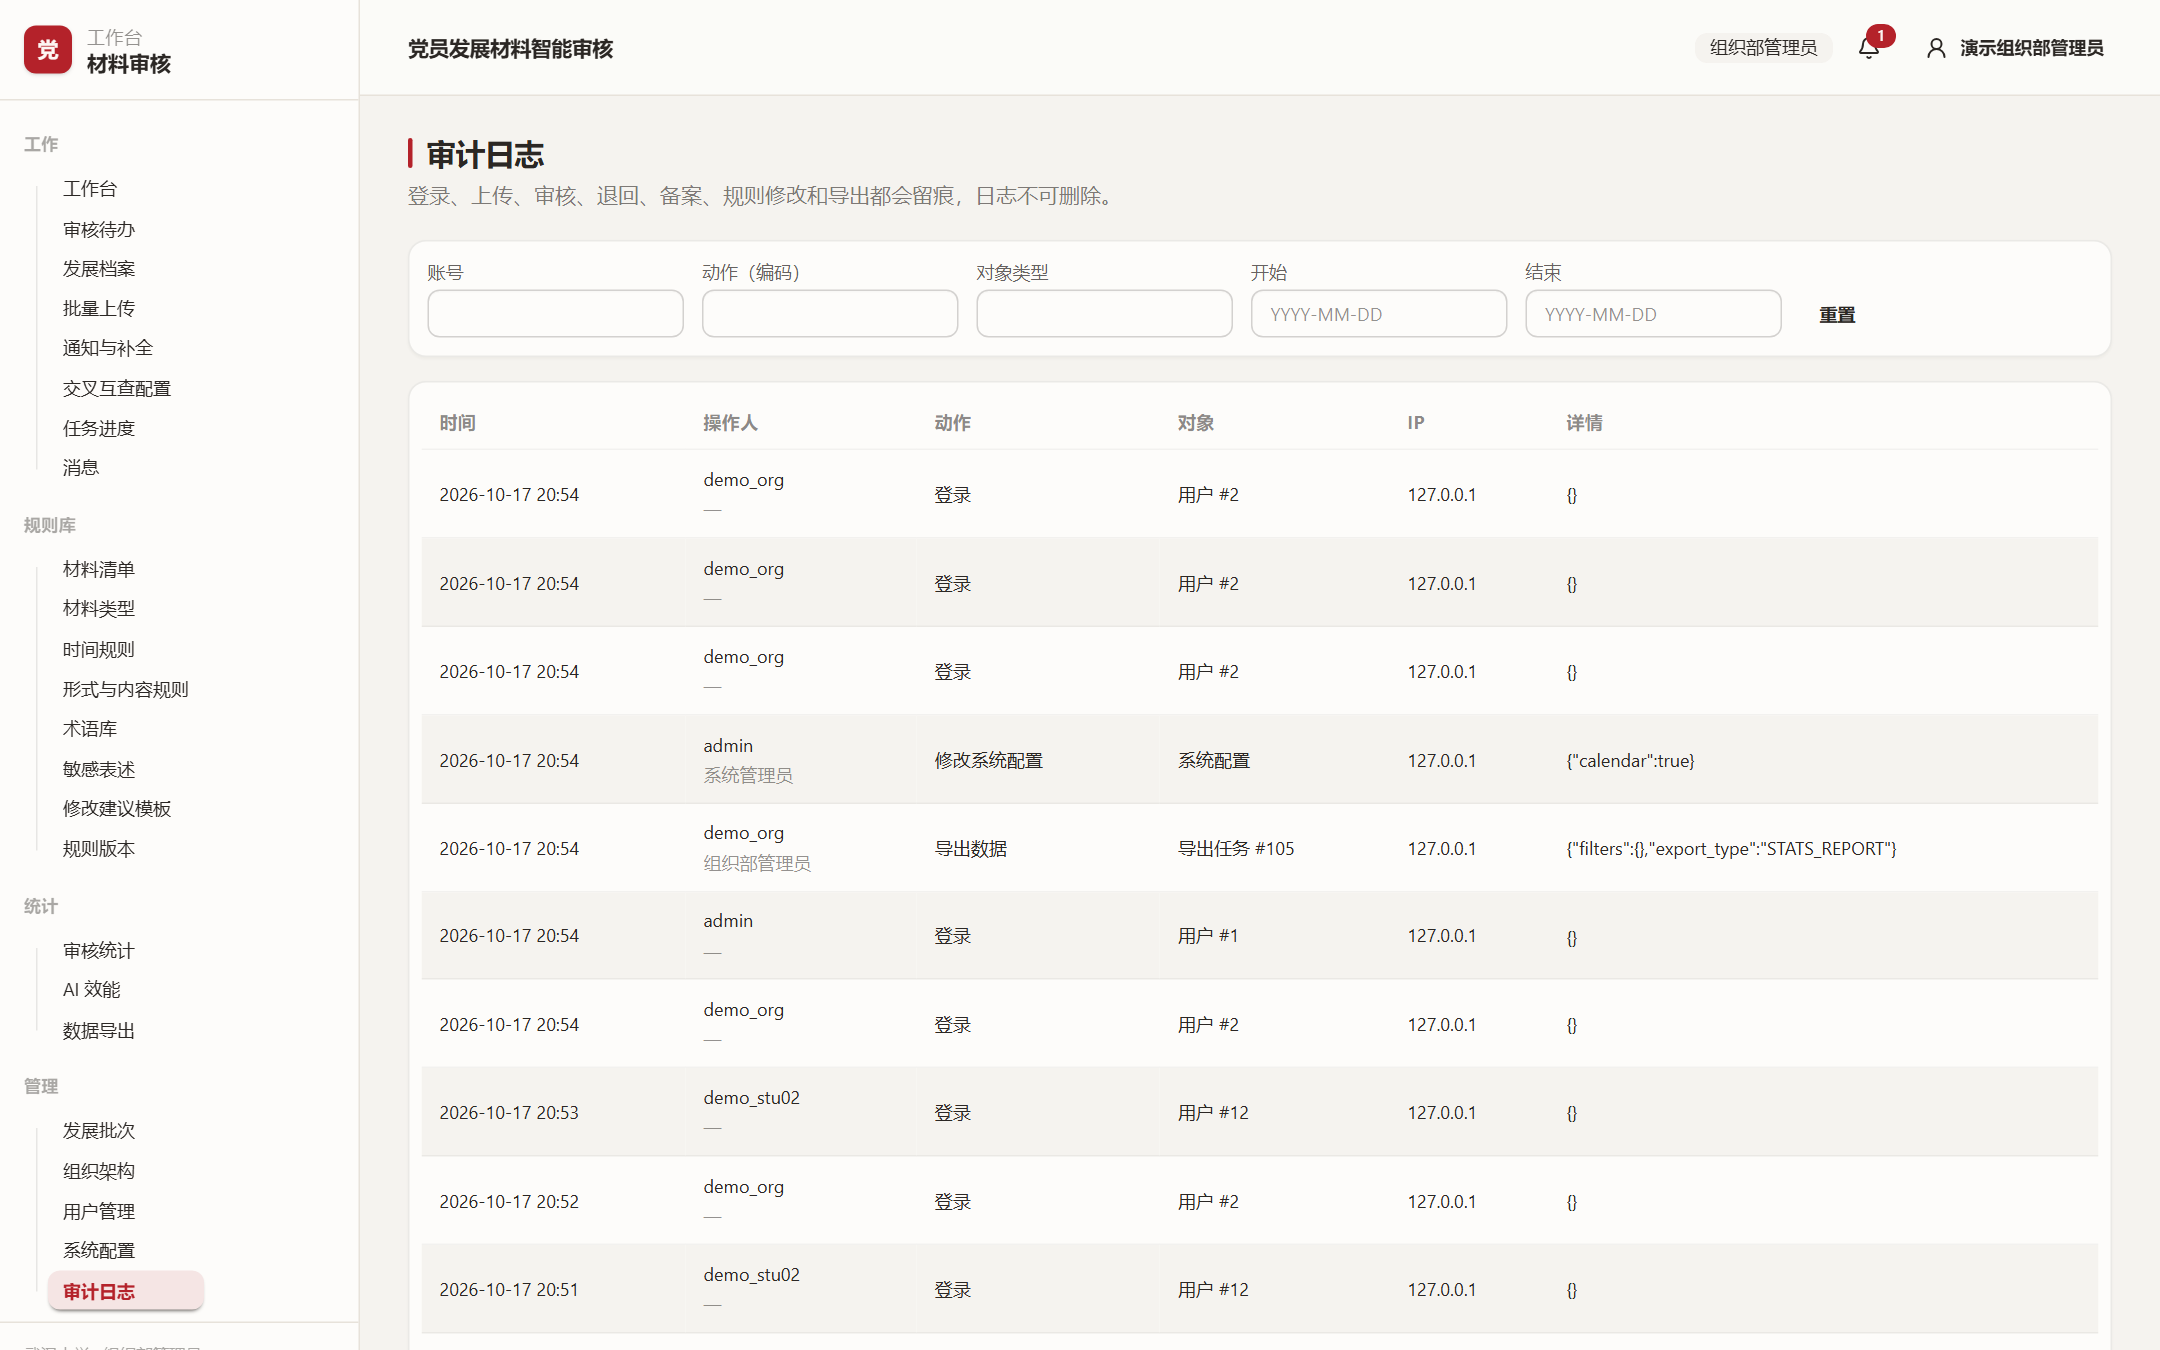
\includegraphics[width=\textwidth]{../figures/shot_audit_logs.png}
    \caption{审计日志}
    \label{fig:ui-audit}
  \end{minipage}
\end{figure}

\subsection{关键实现难点小结}

除前述 OCR 与并发问题外，实现中还发现并解决了两个影响可用性的问题。其一是前端组件库升级导致的表单布局错乱：所用 daisyUI 5 移除了旧版的表单容器类，标签与输入框挤在同一行，涉及登录、改密、筛选栏等九个文件；通过在全局样式中补齐这两个类的定义（标签在上、输入框占满宽度）统一修复，并逐页截图核对。其二是无数据库时测试挂起：数据库不可达时连接会长时间等待，测试套件无法结束；给连接增加 10 秒连接超时，并让冒烟测试在启动前先探测一次数据库、连不上则跳过，测试从超过 5 分钟未结束变为 12 秒完成，同时使生产环境数据库不可达时能快速失败而不是悬挂。

\clearpage

\section{系统测试}

\subsection{测试环境与测试方法}

系统测试在 Windows 11 环境下进行，环境配置如表~\ref{tab:testenv} 所示。数据库使用 PostgreSQL 16.15 的独立二进制，端口 5432；主服务运行于 127.0.0.1:8000，完整链路回归与接口探针在独立空库上另起 127.0.0.1:8001 临时实例执行，测试结束后即行停止并清理临时库。

\begin{table}[H]
  \centering
  \caption{测试环境配置}
  \label{tab:testenv}
  \begin{tabular}{ll}
    \toprule
    项目 & 配置 \\
    \midrule
    操作系统 & Windows 11 \\
    后端运行时 & Python 3.13.12 \\
    前端运行时 & Node.js 24 / npm \\
    数据库 & PostgreSQL 16.15（独立二进制，端口 5432） \\
    后端服务 & uvicorn，127.0.0.1:8000（回归临时实例 8001） \\
    OCR 组件 & PaddleOCR 3.5.0 / PaddlePaddle 3.3.1（可选，本轮未安装） \\
    \bottomrule
  \end{tabular}
\end{table}

测试流程为：安装后端与前端依赖并构建前端产物；在数据库可用与不可用两种条件下运行后端单元测试；随后后台启动后端服务进行探活，再用接口级端到端脚本以真实 HTTP 请求覆盖全部角色的主要业务链路；最后进行界面截图核对并关闭服务进程。为保证结果不依赖残留状态，每一轮回归都在全新空库上从建表、写入默认规则、初始化演示数据开始执行。

\subsection{构建与服务验证}

后端依赖清单共固定 18 个依赖版本，安装一次通过；前端依赖安装成功且无已知漏洞告警；OCR 组件体积较大，作为可选依赖单独安装，不在依赖清单内，未安装时系统自动降级为文本层解析。前端使用 Vite 构建约 1 秒完成，产物由后端同源托管。后端首次启动时自动完成数据库建表，写入 R-T01--R-T23、R-F01--R-F09、R-C01--R-C10 共 42 条默认规则并生成规则版本 v1，创建初始管理员账号，同时启动 2 个后台任务工作线程。

服务探活结果如表~\ref{tab:probe} 所示。服务可用性与安全边界均符合设计：健康检查能同时报告数据库与 OCR 状态；未认证请求被正确拒绝；静态资源仅暴露前端构建产物，存储目录不对外；进程关闭后端口无响应，无残留服务。

\begin{table}[H]
  \centering
  \caption{服务探活结果}
  \label{tab:probe}
  \begin{tabular}{p{4.4cm}p{3.0cm}p{6.4cm}}
    \toprule
    探测项 & 预期 & 实测结果 \\
    \midrule
    GET /api/health & 200 且数据库可用 & 200，status 与 db 均为 ok，version 1.0.0，llm\_enabled=false \\
    GET / & 前端单页应用首页 & 200 \\
    GET /docs & 在线接口文档可用 & 200，接口数不少于 90 \\
    GET /student/\allowbreak self-check & 前端路由回退 & 200，返回前端首页 \\
    GET /api/archives（无令牌） & 拒绝访问 & 401，错误码 40100 \\
    GET /storage/.secret & 不暴露存储目录 & 返回前端首页而非文件内容 \\
    关闭进程后访问端口 & 无响应 & 连接失败，无残留进程 \\
    \bottomrule
  \end{tabular}
\end{table}

\subsection{单元测试与端到端回归}

后端测试使用 pytest 执行：在独立 PostgreSQL 测试库上，45 项测试全部通过，其中 26 项为依赖数据库的集成回归，使用随机临时 schema，结束后仅移除该临时 schema；数据库不可用时，18 项基础用例通过、26 项数据库用例按设计跳过，整套测试约 2 秒完成。前端另有 6 项单元测试，覆盖并发刷新、业务失败重放、迟到 401 等请求竞态场景，以及登录白名单与文件下载错误解析，全部通过。

端到端回归脚本以真实 HTTP 请求覆盖账号权限、档案材料、解析校验、五级审核、整改闭环、规则库与统计等场景。最终一轮在全新空库上的结果为 23 项断言全部通过（共 67 次 HTTP 请求），后台任务无遗留失败。回归主线为：首次改密、上传 DOCX、后台解析、鉴权预览、AI 自查、学生回复阻断问题、提交、按审核意见退回并生成通知、重新提交与自动复核、人工接管、支部通过、交叉互查通过、学院复审通过、组织部备案、自动创建下一阶段提交包，最后验证备案后材料修改被拒绝。另有只读探针补充验证角色隔离与备案后不可变，共 21 项全部通过：非法或伪造角色头一律返回当前角色无效，学生读取他人提交包返回不存在，支部之间档案不可见，互查账号仅见配对支部且排除本支部；备案后修改材料类型、解析结果、上传新版本、删除材料、整改回复、重新提交与重复备案均被拒绝。

大模型链路使用本地模拟端点单独验证 15 项并全部通过：连通性测试可用，不可达端点返回失败而不抛服务错误，配置写入后健康检查反映已启用，报告模式为 RULE\_LLM 且记录实际模型名，三条语义规则产出结论并进入问题清单，语义问题全部标注需人工研判，端点停用后检查任务仍以成功状态完成，失败规则降级为跳过，配置可复原。

\subsection{功能验证}

功能验证逐条对照需求文档的必做功能清单，依据取自端到端脚本中实际通过的检查项与专项验证，主要结果汇总于表~\ref{tab:func}。

\begin{longtable}{p{2.1cm}p{10.0cm}p{1.9cm}}
  \caption{功能验证结果汇总}\label{tab:func}\\
  \toprule
  功能域 & 主要验证内容 & 结论 \\
  \midrule
  \endfirsthead
  \multicolumn{3}{r}{\small 续表~\thetable}\\
  \toprule
  功能域 & 主要验证内容 & 结论 \\
  \midrule
  \endhead
  账号、权限与审计 & 登录登出、密码连续错误 5 次锁定、账号开通不开放注册、首次登录强制改密、角色与数据范围授权（学生仅能访问本人档案、跨支部访问不可见、本支部不能交叉互查、多角色可切换）、操作审计日志覆盖登录、上传、审核、导出与规则变更，无删除接口 & 通过 \\
  基础数据 & 组织架构增改查、用户新增与停用与重置密码、Excel 批量导入及逐行预校验、发展批次与各级审核截止日、演示数据初始化约 13 秒生成 9 个组织、33 个账号、24 份档案、72 个提交包、84 份材料，104 个后台任务全部\allowbreak 完成 & 通过 \\
  档案与材料 & 发展档案与审核历史、21 个阶段进度节点时间轴、四种格式材料上传（非法格式拒绝）、压缩包批量归档与未匹配文件单列、材料在线预览与鉴权下载（匿名访问拒绝）、材料版本管理与整改前后对比 & 通过 \\
  解析与智能校验 & PDF 与 Word 文本层解析、扫描件 OCR 识别并抽取落款日期（历史环境验证）、未安装 OCR 时的降级提示（本轮验证）、解析结果人工校正（时间节点校正强制填写原因）、材料种类识别与份数统计、完整性补全清单、时间与形式规则校验（演示数据命中）、印章检测、内容语义核查（提示词模板调用、失败降级为跳过）、意识形态表述提示人工研判、问题汇总与标准化修改建议（21/21 条附建议）、批量审核压测、整改后自动复核、问题人工确认与误报驳回 & 通过（语义核查经本地模拟端点验证，真实模型效果见 5.6 节） \\
  多级审核与整改闭环 & 审核待办与审核工作区、五级审核链路完整跑通、人工接管（需接管未改判时拒绝通过）、批量审核自动跳过阻断与待接管项、审核流转留痕、整改通知生成与 Word/PDF 导出、学生整改闭环（未回复问题拦截重新提交）、站内消息通知 & 通过 \\
  规则库 & 五个阶段材料清单、24 种材料类型、22 个时间节点、23 条时间规则配置；政治术语与敏感表述库增删改查及导入导出；修改建议模板库；规则修改即生成新版本并在报告中\allowbreak 留痕 & 通过 \\
  统计与系统 & 工作台按角色显示待办与问题分布、高频规则按数据范围统计、审核统计看板（分类、级别、支部、阶段、流转趋势、平均时长）、AI 效能统计、去隐私导出与异步报表导出、AI 服务配置（密钥不回显）、系统参数与任务监控\allowbreak 重试 & 通过 \\
  \bottomrule
\end{longtable}

\subsection{缺陷发现与修复}

自测过程中发现并修复了 10 项缺陷，每项修复后都在全新空库上重跑端到端回归确认。其中影响最大的三项如下。

（1）批量审核父任务并发收尾缺陷。批量 AI 审核由父任务与子任务两级组成，两个后台工作线程并发执行同一批次时，可能各自读取不到对方尚未提交的子任务状态，导致父任务永远停留在运行中状态。该缺陷在回归中约每四轮复现一次，专项压测中 60 个批次有 9 个卡死。修复方案是在父任务收尾前先对父任务行加行级锁，再统计子任务状态，使两个线程串行完成判定。第一版使用排他行锁，与子任务外键持有的共享锁冲突，反而产生了死锁（数据库日志记录 58 次死锁），随后改用冲突更小的锁模式，修复后压测 60 个批次全部完成，0 死锁、0 错误。

（2）扫描件 OCR 不可用。该问题有两层根因：其一，引擎初始化按旧版接口编写，而实际安装的是 3.5.0 版本，初始化抛出的异常被静默捕获并降级为未启用 OCR，改用新版本接口并关闭不兼容的加速选项后恢复；其二，OCR 模型在服务进程内加载时会导致整个进程无回溯退出，排查确认是引擎原生运行时与服务进程不兼容，最终把 OCR 放入独立子进程池执行，子进程异常只影响当次识别，不再危及服务本身。修复后学生上传扫描件可自动完成解析、分类与日期抽取，单页识别约 4 秒，首次加载模型约 30 秒。

（3）数据库不可达时测试挂起。数据库连接不可达时驱动会长时间等待，单元测试超过 5 分钟仍未结束。通过为连接设置 10 秒超时，并让冒烟测试在探测到数据库不可用时按设计跳过，测试在无数据库环境下 12 秒内完成；该修复同时使生产环境在数据库故障时快速失败而不是悬挂。

其余修复包括：规则修改接口未写审计日志（补齐四类规则变更的审计记录）；工作台高频规则与问题分布未按数据范围过滤（改为按角色可见范围统计）；统计看板的流转趋势与平均审核时长恒为空（改为由审核记录实时计算）；OCR 输出的全角数字导致日期无法识别（匹配前统一换算为半角，并补充单元测试）；前端组件库升级导致的表单标签布局错乱（补齐全局样式并逐页截图核对）；整改问题与材料归属未校验（原实现只校验问题属于同一提交包，可用甲材料的新版本把乙材料的问题标记为已整改，改为在写入文件前校验问题的有效性与材料归属，并补充回归用例）；内容语义核查未接入检查流程（规则库中的三条语义规则虽已配置模型引擎，但检查流程从未真正调用模型，配置后也只会静默通过；接入后按内容核查模板调用并将结果映射为问题，语义结论一律转人工研判，同时改为单次尝试、首次失败即停止后续调用，修复了端点不可达时检查任务长时间停留在运行中的问题，并在报告中记录实际模型名）。

\subsection{已知问题与测试结论}

测试中确认的已知问题如下：一是大模型尚未接入真实模型，语义核查链路虽已用本地模拟端点完成配置、调用、降级与追溯验证（模型名写入报告、失败规则降级为跳过、任务不中断），但真实模型的语言表述核查、要素理解与建议生成效果尚未评估，需配置真实接口后建立评测集量化；二是 OCR 组件不在依赖清单内且首次加载较慢，本轮验证环境未安装，扫描件走降级提示，手写体识别准确率未做专项评估；三是手写签名检测目前为启发式实现，未用真实签名样本评估准确度，低置信度时会提示人工核对；四是演示数据中每个提交包均预设了阻断问题，首次使用时需先完成问题处理与人工接管才能走向通过，这与"AI 不替代人工判断"的设计一致，但会带来一定的上手成本；五是平均审核时长按相邻流转记录的时间差计算，自测中流转在数秒内完成，显示为接近 0 小时，真实使用后才有参考意义；六是学生角色当前可读取规则库，若需收紧权限可进一步调整；此外测试依赖存在一条弃用告警，只影响测试代码，不影响系统运行。界面验证以真实页面截图核对为主，未做真实浏览器中的逐项交互与无障碍专项测试。

综合来看，系统在功能、权限、数据范围、状态流转、降级与人工接管等方面均达到设计要求：全部必做功能实现并通过端到端验证，五级审核链路与整改闭环完整可用，AI 输出始终以建议形式呈现、关键结论保留人工确认；遗留问题集中在真实大模型效果评估、OCR 与签名精度评估、界面交互测试三个方面，不影响核心链路的正确性。

\clearpage

\section{总结与展望}

\subsection{工作总结}

本文围绕高校党员发展材料审核的实际需求，设计并实现了"AI 辅助 + 人工确认"的党员发展材料智能审核工作台。主要工作可归纳为四个方面。

（1）业务建模与流程抽象。梳理了申请入党、确定入党积极分子、确定发展对象、接收预备党员、预备党员转正五个发展阶段的全部材料要求与时间约束，抽象出发展档案、提交包、材料版本、时间节点、AI 报告、问题、审核记录、规则版本等核心业务对象，设计了以提交包为流转单元、以问题为闭环对象的状态机模型，实现了学生自查、党支部初审、支部交叉互查、学院党委复审、学校组织部备案的五级审核链路与退回整改闭环。

（2）可配置的审核规则体系与智能审核引擎。设计了包含 14 个原子算子的时间规则领域特定语言，把培养周期、阶段间隔、公示时限等程序性要求表达为可配置、可版本化的规则，内置 23 条时间规则、9 条形式规范规则与 10 条内容规范规则；实现了"解析—理解—校验—汇总—结论"五阶段审核流水线，支持 PDF、Word、图片多格式解析与扫描件 OCR、材料种类识别、结构化要素抽取、跨来源时间节点合并与冲突判定，输出可定位到原文、附标准化修改建议的问题清单。

（3）"可信 AI"机制设计与工程实现。坚持"规则引擎为主、大语言模型为辅、人工接管兜底"的架构：可规则化、可解释、可审计的检查全部由规则引擎完成；语义性、开放性的问题交给大语言模型但只作为提示；置信度不足、跨来源冲突、关键阶段等场景强制进入人工接管，审核人员必须写明理由改判后方可放行。系统基于 FastAPI、React 与 PostgreSQL 实现，数据库共 35 张表，接口 90 余个，通过行级锁与任务队列保证并发一致性，通过审计日志、材料版本管理与规则版本快照保证全过程可追溯。

（4）系统测试与缺陷修复。完成了后端 45 项单元与集成测试、23 项 HTTP 全链路断言与 36 项接口探针（共 104 项通过、0 项失败），前端 6 项单元测试同步通过，并通过专项压测验证了批量审核的并发正确性；修复了并发父任务收尾、扫描件 OCR 兼容性、全角数字识别、统计口径、表单布局、整改问题归属校验、大模型语义核查接入等 10 项缺陷。

\subsection{不足与展望}

受测试条件限制，本文工作仍存在若干不足，也对应着后续的改进方向。第一，语义核查链路虽已用本地模拟端点验证（含失败降级与模型名追溯），但尚未接入真实模型，语义核查的准确率与误报率缺乏量化评估，后续需要配置真实接口，针对内容语义核查、要素理解与整改建议生成建立评测集，量化问题召回率与误报率变化；同时可探索把发展阶段业务细则构建为检索增强生成的知识库，提升建议生成与条款引用的准确性。第二，OCR 与视觉检测的精度评估不充分，手写体识别与手写签名检测尚未用真实样本评估，后续可采集标注样本进行专项评估，必要时对识别模型做领域微调。第三，测试以功能与并发正确性为主，更大数据量、更高并发下的性能表现，以及前端在真实浏览器中的交互体验与无障碍支持，还需要补充专项测试。第四，规则库目前通过管理界面逐条维护，后续可引入规则冲突检测与规则影响分析，进一步降低规则维护门槛。总体上，本文验证了"规则引擎 + 大语言模型 + 人工接管"组合在高敏感材料审核场景的可行性，后续工作将围绕模型能力实测与精度评估继续完善。

\clearpage

\begin{thebibliography}{99}

\bibitem{ppocr2020}
Du Y, Li C, Guo R, et al. PP-OCR: a practical ultra lightweight OCR system[EB/OL]. arXiv:2009.09941, 2020.

\bibitem{ppocrv3_2022}
Li C, Liu W, Guo R, et al. PP-OCRv3: more attempts for the improvement of ultra lightweight OCR system[EB/OL]. arXiv:2206.03001, 2022.

\bibitem{layoutlmv3_2022}
Huang Y, Lv T, Cui L, et al. LayoutLMv3: pre-training for document AI with unified text and image masking[C]//Proceedings of the 30th ACM International Conference on Multimedia. New York: ACM, 2022: 4083--4091.

\bibitem{donut_2021}
Kim G, Hong T, Yim M, et al. OCR-free document understanding transformer[EB/OL]. arXiv:2111.15664, 2021.

\bibitem{vaswani_2017}
Vaswani A, Shazeer N, Parmar N, et al. Attention is all you need[C]//Advances in Neural Information Processing Systems (NeurIPS). 2017.

\bibitem{bert_2019}
Devlin J, Chang M W, Lee K, et al. BERT: pre-training of deep bidirectional transformers for language understanding[C]//Proceedings of the 2019 Conference of the North American Chapter of the Association for Computational Linguistics: Human Language Technologies. Stroudsburg: ACL, 2019: 4171--4186.

\bibitem{rag_2020}
Lewis P, Perez E, Piktus A, et al. Retrieval-augmented generation for knowledge-intensive NLP tasks[EB/OL]. arXiv:2005.11401, 2020.

\bibitem{cner_2019}
Zhao H, Xu M, Cao J. Pre-trained language model transfer on Chinese named entity recognition[C]//2019 IEEE International Conference on High Performance Computing and Communications, IEEE International Conference on Smart City, IEEE International Conference on Data Science and Systems (HPCC/SmartCity/DSS). IEEE, 2019.

\bibitem{acc_2015}
Pauwels P, Zhang S. Semantic rule-checking for regulation compliance checking: an overview of strategies and approaches[C/OL]. Ghent University, 2015.

\bibitem{acc_2022}
Zhang Z, Nisbet N, Ma L, et al. Capabilities of rule representations for automated compliance checking in healthcare buildings[J]. Automation in Construction, 2023, 146: 104688.

\end{thebibliography}

\end{document}
